\documentclass[11pt]{article}
\usepackage[margin=1in]{geometry}
\usepackage{amsmath,amssymb,amsthm,booktabs,graphicx,enumitem,mathtools}
\usepackage[dvipsnames]{xcolor}
\usepackage[most]{tcolorbox}
\usepackage{fancyhdr}
\usepackage{hyperref}
% GENERATED by verification/verify_all.py -- do not edit by hand.
% Every number here is read off the certificates on disk.

\newcommand{\NtileThree}{23}
\newcommand{\LvalThree}{21}
\newcommand{\LmaxThree}{43}
\newcommand{\NtileFour}{33}
\newcommand{\LvalFour}{29}
\newcommand{\LmaxFour}{61}
\newcommand{\NtileFive}{21}
\newcommand{\LvalFive}{54}
\newcommand{\LmaxFive}{75}
\newcommand{\NtileThreeFour}{56}
\newcommand{\NtileAll}{77}
\newcommand{\SettleThree}{21}
\newcommand{\SettleFour}{29}
\newcommand{\SettleFive}{162}
\newcommand{\NcertGN}{17}
\newcommand{\GNlo}{17}
\newcommand{\GNhi}{33}
\newcommand{\MaxAlpha}{1.0\times10^{-9}}
\newcommand{\RamLastOne}{14}
\newcommand{\RamCountOne}{9}
\newcommand{\RamLastTwo}{23}
\newcommand{\RamCountTwo}{19}
\newcommand{\RamLastThree}{32}
\newcommand{\RamCountThree}{18}
\newcommand{\RamLastFour}{42}
\newcommand{\RamCountFour}{34}
\newcommand{\RamLastFive}{50}
\newcommand{\RamCountFive}{28}
\newcommand{\RamLastSix}{49}
\newcommand{\RamCountSix}{20}
\newcommand{\RamLastSeven}{70}
\newcommand{\RamCountSeven}{39}
\newcommand{\RamLastEight}{49}
\newcommand{\RamCountEight}{16}
\newcommand{\RamLastNine}{90}
\newcommand{\RamCountNine}{50}
\newcommand{\RamLastTen}{52}
\newcommand{\RamCountTen}{14}
\newcommand{\RamTotal}{247}
\newcommand{\RamKmax}{10}
\newcommand{\RamCases}{458}
\newcommand{\RamBoundTwo}{23}
\newcommand{\RamBoundThree}{32}
\newcommand{\RamBoundFour}{42}
\newcommand{\RamDirichlet}{231}
\newcommand{\RamAllTotal}{460}
\newcommand{\RamAllIso}{324}
\newcommand{\RamAllMaxN}{112}
\newcommand{\RamAllMaxK}{45}
\newcommand{\RamAllSizes}{80}
\newcommand{\RamAllCases}{13110}
\newcommand{\RatClassTwo}{7,9,15,20}
\newcommand{\RatClassThree}{10,24,42}
\newcommand{\RatClassFour}{60,70,90}
\newcommand{\RatClassFive}{24,126}
\newcommand{\RatClassSix}{\text{none}}
\newcommand{\RatClassSeven}{120}
\newcommand{\TileAllK}{9}
\newcommand{\Nchecks}{150}


\pagestyle{fancy}
\fancyhf{}
\fancyhead[L]{\small\scshape Mathematical Foundations Guide}
\fancyhead[R]{\small\scshape Ramanujan $P(n,k)$ $\bullet$ Zero Forcing $\bullet$ Maximum Nullity}
\fancyfoot[C]{\thepage}
\renewcommand{\headrulewidth}{0.4pt}

\hypersetup{
  colorlinks=true,
  linkcolor=NavyBlue,
  urlcolor=NavyBlue,
  citecolor=NavyBlue
}

\definecolor{defblue}{RGB}{20,60,110}
\definecolor{deffill}{RGB}{232,239,248}
\definecolor{intuorange}{RGB}{200,110,20}
\definecolor{intufill}{RGB}{253,243,227}
\definecolor{thmgreen}{RGB}{25,100,60}
\definecolor{thmfill}{RGB}{233,245,237}
\definecolor{calloutframe}{RGB}{120,40,40}
\definecolor{calloutfill}{RGB}{250,235,235}

\newtcolorbox{defbox}[1]{
  colback=deffill,
  colframe=defblue,
  fonttitle=\bfseries,
  title={#1},
  breakable,
  boxrule=0.8pt,
  arc=3pt
}

\newtcolorbox{intubox}[1]{
  colback=intufill,
  colframe=intuorange,
  fonttitle=\bfseries,
  title={#1},
  breakable,
  boxrule=0.8pt,
  arc=3pt
}

\newtcolorbox{thmbox}[1]{
  colback=thmfill,
  colframe=thmgreen,
  fonttitle=\bfseries,
  title={#1},
  breakable,
  boxrule=0.8pt,
  arc=3pt
}

\newtcolorbox{callbox}[1]{
  colback=calloutfill,
  colframe=calloutframe,
  fonttitle=\bfseries,
  title={#1},
  breakable,
  boxrule=0.8pt,
  arc=3pt
}

\title{\vspace{-1.2cm}\textbf{\huge Complete Mathematical Foundations \&\\[4pt]
Derivations Guide}\\[10pt]
\Large A Comprehensive, High-School-to-Advanced Reference for\\[3pt]
\emph{Which Graphs Satisfy the Riemann Hypothesis? Ramanujan Generalized Petersen Graphs, and the Zero Forcing Number and Maximum Nullity of the Same Family}}

\author{\textbf{Research Reference Manual}\\[3pt]
Graph Theory $\bullet$ Linear Algebra $\bullet$ Cyclotomy $\bullet$ Interval Arithmetic\\
Cyclic Covers $\bullet$ Ihara Zeta Functions $\bullet$ Expander Graphs\\[6pt]
\textbf{Aryan Padarthi}}
\date{October 2026}

\begin{document}
\maketitle

\begin{abstract}
\noindent
This reference explains \textbf{every mathematical object, equation, variable, derivation and proof} used in the research project \emph{``Which graphs satisfy the Riemann Hypothesis? A certified classification of the Ramanujan generalized Petersen graphs, and the exact zero forcing number and maximum nullity of the same family''}. It starts from high-school material --- graphs, clock arithmetic, matrices, complex numbers --- and builds each object from first principles, with a precise definition, an intuition box, and a fully worked numerical example that can be checked by hand.

The project has two halves and one engine. The engine is the observation that the generalized Petersen graph $P(n,k)$ is a \emph{cyclic cover} of a two-vertex base graph, so that every question about it decomposes over the characters of $\mathbb Z_n$ into $2\times2$ blocks.

\begin{enumerate}[leftmargin=*,nosep]
  \item \textbf{Part II (zero forcing and maximum nullity), Sections 2--11.} The zero forcing colour-change rule; the inequality $M(G)\le Z(G)$; the rotation bootstrap giving $Z(P(n,k))\le2k+2$; why combinatorial lower bounds fail; the \emph{monodromy ceiling} --- eliminating the inner coordinates of \emph{any} matrix on the $P(n,k)$ pattern leaves one recurrence of order $2k+2$, so the certificate method either matches the upper bound exactly or cannot; period-one certificates and the Chebyshev symbol; cyclotomic integer certificates; \emph{tiles} whose monodromy is the identity, which settle every $n\ge17$ at $k=3$ and every $n\ge29$ at $k=4$; Krawczyk certification evaluated in exact rational arithmetic; the general theory of cyclic covers, including two refutations of the project's own conjectures; and the period-one ceiling that explains the two cases the method cannot reach.
  \item \textbf{Part I (the graph Riemann Hypothesis), Section 12.} The Ihara zeta function; why its Riemann Hypothesis is the Ramanujan condition $|\lambda|\le2\sqrt2$; the integer polynomial $D_k$ that decides it with no radicals; the corner criterion $Q(x,y)\ge0$ that does not involve $k$; the uniform and Dirichlet finiteness bounds; the complete certified classification --- exactly $\RamAllTotal$ pairs $(n,k)$, $\RamAllIso$ graphs up to isomorphism, none past $n=\RamAllMaxN$ or $k=\RamAllMaxK$; and why no cyclic cover of any fixed cubic base gives an infinite Ramanujan family.
  \item \textbf{Verification, Section 13.} What ``certified'' means in this project, what the $\Nchecks$-check suite does and does not catch, and the claims of our own that it or an outside reader refuted.
\end{enumerate}

\noindent
Every number in a worked example was computed by the project's own code and re-derived here by hand. Every claim is labelled by the standard it meets --- proved, proved by exact certificate, proved by interval certification, numerical, conjectural, or refuted --- in Section 16, matching the Status section of the paper.
\end{abstract}


\tableofcontents
\newpage

%% =========================================================================
%% SECTION 1: HIGH SCHOOL FOUNDATION PRIMER
%% =========================================================================
\section{Introduction \& High School Foundation Primer}

Everything in this project rests on four fundamental pillars taught in high school: graph theory, clock arithmetic, linear algebra, and complex numbers. We build each from the ground up.

\subsection{Graphs, Sets, and Networks}

\begin{defbox}{Definition 1.1: Graph, Vertices, and Edges}
A \textbf{graph} $G = (V, E)$ is a discrete structure consisting of:
\begin{itemize}[leftmargin=*,nosep]
  \item A set of \textbf{vertices} (or nodes) $V = \{v_1, v_2, \dots, v_N\}$ representing discrete entities. The number of vertices is denoted $|V| = N$.
  \item A set of \textbf{edges} $E = \{e_1, e_2, \dots, e_m\}$ representing pairwise connections. Each edge $e \in E$ is an unordered pair $(u, v)$ with $u, v \in V$. We write $uv \in E$ or $u \sim v$ to denote that $u$ and $v$ are adjacent. The number of edges is denoted $|E| = m$.
\end{itemize}
\end{defbox}

\begin{defbox}{Key Graph Variables \& Local Structure}
\begin{itemize}[leftmargin=*,nosep]
  \item \textbf{Open Neighbourhood} $N(u)$: The set of all vertices directly connected to $u$:
  \begin{equation}
    N(u) = \{v \in V \mid uv \in E\}.
  \end{equation}
  \item \textbf{Closed Neighbourhood} $N[u]$: The neighbourhood of $u$ including $u$ itself: $N[u] = N(u) \cup \{u\}$.
  \item \textbf{Degree} $\deg(u)$: The number of edges connected to vertex $u$:
  \begin{equation}
    \deg(u) = |N(u)|.
  \end{equation}
  \item \textbf{$d$-Regular Graph}: A graph where every vertex has the exact same degree: $\deg(u) = d$ for all $u \in V$.
  \item \textbf{Cubic Graph}: A 3-regular graph ($\deg(u) = 3$ for all $u \in V$). Every vertex touches exactly three neighbours.
  \item \textbf{Adjacency Matrix} $A \in \mathbb{R}^{N \times N}$: A symmetric table of $0$s and $1$s where:
  \begin{equation}
    A_{uv} = \begin{cases} 1 & \text{if } uv \in E, \\ 0 & \text{otherwise}. \end{cases}
  \end{equation}
  \item \textbf{Degree Matrix} $D \in \mathbb{R}^{N \times N}$: A diagonal matrix whose diagonal entries are the vertex degrees: $D_{uu} = \deg(u)$, and $D_{uv} = 0$ for $u \ne v$.
\end{itemize}
\end{defbox}

\begin{intubox}{Intuition \& High School Analogy: What is a Cubic Graph?}
Think of a road network or an electrical power grid:
\begin{itemize}[leftmargin=*,nosep]
  \item \textbf{Vertices ($V$)}: Road intersections or power substations.
  \item \textbf{Edges ($E$)}: Streets connecting intersections or high-voltage transmission lines.
  \item \textbf{Cubic Graph}: Picture a city where \emph{every single intersection} is a 3-way fork (a T-junction or Y-junction). There are never dead ends (degree 1), simple straight roads (degree 2), or 4-way cross streets (degree 4).
\end{itemize}
\end{intubox}

\begin{callbox}{Worked Numerical Example 1.1: A Concrete 4-Vertex Graph and its Matrices}
Let $V = \{1, 2, 3, 4\}$ and $E = \{(1,2), (2,3), (3,4), (4,1), (1,3)\}$.
\begin{itemize}[leftmargin=*,nosep]
  \item Neighbours of vertex 1: $N(1) = \{2, 3, 4\} \implies \deg(1) = 3$.
  \item Neighbours of vertex 2: $N(2) = \{1, 3\} \implies \deg(2) = 2$.
  \item Neighbours of vertex 3: $N(3) = \{1, 2, 4\} \implies \deg(3) = 3$.
  \item Neighbours of vertex 4: $N(4) = \{1, 3\} \implies \deg(4) = 2$.
\end{itemize}
The $4 \times 4$ \textbf{adjacency matrix} $A$ and \textbf{degree matrix} $D$ are:
\begin{equation}
  A = \begin{pmatrix}
    0 & 1 & 1 & 1 \\
    1 & 0 & 1 & 0 \\
    1 & 1 & 0 & 1 \\
    1 & 0 & 1 & 0
  \end{pmatrix}, \qquad
  D = \begin{pmatrix}
    3 & 0 & 0 & 0 \\
    0 & 2 & 0 & 0 \\
    0 & 0 & 3 & 0 \\
    0 & 0 & 0 & 2
  \end{pmatrix}.
\end{equation}
The standard combinatorial \textbf{Laplacian matrix} $L = D - A$ evaluates directly to:
\begin{equation}
  L = D - A = \begin{pmatrix}
    3 & -1 & -1 & -1 \\
    -1 & 2 & -1 & 0 \\
    -1 & -1 & 3 & -1 \\
    -1 & 0 & -1 & 2
  \end{pmatrix}.
\end{equation}
Notice that the sum of every row is identically zero: for row 1, $3 + (-1) + (-1) + (-1) = 0$. 
This guarantees that the constant all-ones vector $\mathbf{1} = [1, 1, 1, 1]^T$ is always in the kernel: $L \mathbf{1} = \mathbf{0}$.
\end{callbox}

\subsection{Modular Arithmetic and the Clock Lemma}

\begin{defbox}{Definition 1.2: Modular Arithmetic}
Let $n$ be a positive integer. Two integers $a$ and $b$ are \textbf{congruent modulo $n$}, written
\begin{equation}
  a \equiv b \pmod n,
\end{equation}
if their difference $a - b$ is an integer multiple of $n$. Equivalently, $a$ and $b$ leave the same remainder when divided by $n$.
The set of residue classes is denoted $\mathbb{Z}_n = \{0, 1, 2, \dots, n-1\}$. All additions, subtractions, and multiplications are performed ``wrapping around'' at $n$:
\begin{equation}
  (n-1) + 1 \equiv 0 \pmod n.
\end{equation}
\end{defbox}

\begin{defbox}{Definition 1.3: Greatest Common Divisor and Coprimality}
The \textbf{greatest common divisor} $\gcd(n, k)$ is the largest integer dividing both $n$ and $k$. If $\gcd(n, k) = 1$, we say that $n$ and $k$ are \textbf{coprime} (or relatively prime).
\end{defbox}

\begin{thmbox}{Theorem 1.1: The Clock Orbit Lemma}
Let $n \ge 1$ and $k \ge 1$. Consider the permutation $\tau: \mathbb{Z}_n \to \mathbb{Z}_n$ defined by jumping $k$ steps forward: $\tau(i) \equiv i + k \pmod n$. 
Then the $n$ elements of $\mathbb{Z}_n$ partition into exactly
\begin{equation}
  d = \gcd(n, k)
\end{equation}
disjoint cyclic orbits, each of length $n / d$.
\end{thmbox}

\begin{defbox}{Proof of the Clock Orbit Lemma}
Consider the cyclic subgroup generated by $k$ inside the additive group $(\mathbb{Z}_n, +)$. The order of $k$ modulo $n$ is the smallest positive integer $L$ such that $L \cdot k \equiv 0 \pmod n$. 
This requires $L \cdot k$ to be a common multiple of $k$ and $n$. The least common multiple is $\operatorname{lcm}(n, k) = \frac{n \cdot k}{\gcd(n, k)}$. Therefore:
\begin{equation}
  L = \frac{\operatorname{lcm}(n, k)}{k} = \frac{n}{\gcd(n, k)} = \frac{n}{d}.
\end{equation}
Every orbit of the shift $\tau(i) = i + k$ is a coset of this subgroup, hence has size $L = n/d$. Since the orbits partition the $n$ elements, the total number of disjoint orbits is:
\begin{equation}
  \text{Number of Orbits} = \frac{n}{L} = \frac{n}{n/d} = d = \gcd(n, k). \qedhere
\end{equation}
\end{defbox}

\begin{intubox}{Intuition \& High School Analogy: The 12-Hour Clock}
Stand on the 12-hour clock face $\{0, 1, 2, \dots, 11\}$ and jump by $k$ hours repeatedly:
\begin{itemize}[leftmargin=*,nosep]
  \item \textbf{Case $k=5$}: Start at $0 \to 5 \to 10 \to 3 \to 8 \to 1 \to 6 \to 11 \to 4 \to 9 \to 2 \to 7 \to 0$. You visit all 12 numbers in a single giant loop of length 12. Here $\gcd(12, 5) = 1$, so $d=1$ orbit.
  \item \textbf{Case $k=4$}: Start at $0 \to 4 \to 8 \to 0$. You are trapped in an equilateral triangle of 3 numbers. The other numbers form two parallel triangles: $\{1, 5, 9\}$ and $\{2, 6, 10\}$. Here $\gcd(12, 4) = 4$, so the 12 numbers split into $4$ separate triangular cycles of length 3.
\end{itemize}
\textbf{Why this matters}: In the Generalized Petersen graph $P(n,k)$, the inner vertices are connected by jumping $k$ steps. Therefore, the inner ring is not always one single circle: it shatters into $\gcd(n, k)$ disjoint polygons.
\end{intubox}

\begin{callbox}{Worked Numerical Example 1.2: Explicit Clock Orbits for $n=12$ with $k=5$ vs $k=4$}
Let us write out the exact partition of $\mathbb{Z}_{12} = \{0, 1, 2, \dots, 11\}$ generated by jumping $k$ steps forward:
\begin{itemize}[leftmargin=*,nosep]
  \item \textbf{Coprime Case ($k=5$)}: $\gcd(12, 5) = 1$. The formula predicts $d = 1$ single orbit of length $L = 12 / 1 = 12$.
  Tracing the sequence explicitly:
  \begin{equation}
    0 \xrightarrow{+5} 5 \xrightarrow{+5} 10 \xrightarrow{+5} 3 \xrightarrow{+5} 8 \xrightarrow{+5} 1 \xrightarrow{+5} 6 \xrightarrow{+5} 11 \xrightarrow{+5} 4 \xrightarrow{+5} 9 \xrightarrow{+5} 2 \xrightarrow{+5} 7 \xrightarrow{+5} 0.
  \end{equation}
  The single orbit visits every single element: $\mathcal{O}_0 = \{0, 1, 2, 3, 4, 5, 6, 7, 8, 9, 10, 11\}$.
  \item \textbf{Non-Coprime Case ($k=4$)}: $\gcd(12, 4) = 4$. The formula predicts $d = 4$ disjoint orbits of length $L = 12 / 4 = 3$.
  Computing each orbit starting from the smallest unvisited element:
  \begin{align}
    \mathcal{O}_0 &= \{0, 0+4, 0+8\} = \{0, 4, 8\}, \\
    \mathcal{O}_1 &= \{1, 1+4, 1+8\} = \{1, 5, 9\}, \\
    \mathcal{O}_2 &= \{2, 2+4, 2+8\} = \{2, 6, 10\}, \\
    \mathcal{O}_3 &= \{3, 3+4, 3+8\} = \{3, 7, 11\}.
  \end{align}
  The union $\mathcal{O}_0 \cup \mathcal{O}_1 \cup \mathcal{O}_2 \cup \mathcal{O}_3 = \mathbb{Z}_{12}$ partitions the 12 vertices into 4 disjoint triangles.
\end{itemize}
\end{callbox}

\subsection{Linear Algebra from Scratch}

\begin{defbox}{Definition 1.4: Vectors, Matrices, and Linear Transformations}
\begin{itemize}[leftmargin=*,nosep]
  \item \textbf{Vector} $x \in \mathbb{R}^N$: An ordered list of $N$ real numbers, $x = [x_1, x_2, \dots, x_N]^T$.
  \item \textbf{Matrix} $A \in \mathbb{R}^{N \times N}$: A square array of numbers where $A_{ij}$ is the entry in row $i$ and column $j$. A matrix represents a linear transformation mapping any vector $x \in \mathbb{R}^N$ to a new vector $y = Ax \in \mathbb{R}^N$ via:
  \begin{equation}
    y_i = (Ax)_i = \sum_{j=1}^N A_{ij} x_j.
  \end{equation}
  \item \textbf{Symmetric Matrix}: A matrix where $A_{ij} = A_{ji}$ for all $i, j$, or equivalently $A = A^T$.
\end{itemize}
\end{defbox}

\begin{defbox}{Definition 1.5: Kernel, Nullity, Image, and Rank}
\begin{itemize}[leftmargin=*,nosep]
  \item \textbf{Null Space / Kernel} $\ker(A)$: The set of all vectors that the matrix maps to zero:
  \begin{equation}
    \ker(A) = \{x \in \mathbb{R}^N \mid Ax = \mathbf{0}\}.
  \end{equation}
  \item \textbf{Nullity} $\operatorname{null}(A)$: The dimension of the null space, $\operatorname{null}(A) = \dim(\ker(A))$. It equals the number of linearly independent solutions to the homogeneous linear equation system $Ax = \mathbf{0}$.
  \item \textbf{Image / Column Space} $\operatorname{im}(A)$: The set of all possible outputs $\{Ax \mid x \in \mathbb{R}^N\}$.
  \item \textbf{Rank} $\operatorname{rank}(A)$: The dimension of the column space, $\operatorname{rank}(A) = \dim(\operatorname{im}(A))$.
\end{itemize}
\end{defbox}

\begin{thmbox}{Theorem 1.2: The Rank-Nullity Theorem}
For any linear transformation represented by an $N \times N$ matrix $A$:
\begin{equation}
  \operatorname{rank}(A) + \operatorname{null}(A) = N.
\end{equation}
\end{thmbox}

\begin{intubox}{Intuition \& High School Analogy: The Lossy Camera}
Think of a matrix as a digital camera taking an $N$-dimensional scene and projecting it onto an output screen:
\begin{itemize}[leftmargin=*,nosep]
  \item \textbf{Rank}: The number of dimensions visible in the final photograph.
  \item \textbf{Nullity}: The number of blind spots or collapsed dimensions that are completely crushed to black ($0$).
  \item If $\operatorname{null}(A) = 0$, the camera is perfectly lossless: the only scene that looks black is an empty room ($x=\mathbf{0}$).
  \item If $\operatorname{null}(A) = r > 0$, there exists an entire $r$-dimensional space of non-zero scenes that all produce complete darkness.
\end{itemize}
\textbf{The central challenge}: We want to design the lossiest possible physical machine (maximum nullity) whose wiring diagram strictly obeys our graph.
\end{intubox}

\begin{defbox}{Definition 1.6: Eigenvalues, Eigenvectors, and Multiplicity}
A scalar $\lambda \in \mathbb{C}$ is an \textbf{eigenvalue} of $A$ with non-zero \textbf{eigenvector} $v \ne \mathbf{0}$ if:
\begin{equation}
  Av = \lambda v.
\end{equation}
\begin{itemize}[leftmargin=*,nosep]
  \item \textbf{Geometric Multiplicity} of $\lambda$: The dimension of the eigenspace, $\dim\ker(A - \lambda I)$.
  \item For $\lambda = 0$, the eigenspace is precisely the kernel: $\dim\ker(A - 0 I) = \operatorname{null}(A)$.
  \item For a real symmetric matrix $A = A^T$, all eigenvalues are real, the matrix is orthogonally diagonalizable, and the algebraic multiplicity of every eigenvalue equals its geometric multiplicity.
\end{itemize}
\end{defbox}

\begin{defbox}{Definition 1.7: Companion Matrices and Monodromy Operators}
Consider a linear recurrence relation of order $K$:
\begin{equation}
  x_{i+K} = \sum_{p=0}^{K-1} c_p x_{i+p}.
\end{equation}
We can represent the recurrence as a state-vector update $X_{i+1} = M_i X_i$, where $X_i = [x_i, x_{i+1}, \dots, x_{i+K-1}]^T \in \mathbb{R}^K$ and $M_i$ is a \textbf{companion matrix}:
\begin{equation}
  M_i = \begin{pmatrix}
    0 & 1 & 0 & \cdots & 0 \\
    0 & 0 & 1 & \cdots & 0 \\
    \vdots & \vdots & \vdots & \ddots & \vdots \\
    0 & 0 & 0 & \cdots & 1 \\
    c_0 & c_1 & c_2 & \cdots & c_{K-1}
  \end{pmatrix}.
\end{equation}
Advancing the recurrence across an entire circular loop of length $n$ yields the \textbf{monodromy operator}:
\begin{equation}
  T = M_{n-1} M_{n-2} \cdots M_1 M_0 \in \mathbb{R}^{K \times K}.
\end{equation}
A sequence is $n$-periodic ($X_n = X_0$) if and only if $T X_0 = X_0$, which means $(T - I)X_0 = \mathbf{0}$. Therefore, the number of independent periodic solutions is exactly $\dim\ker(T - I)$.
\end{defbox}

\begin{callbox}{Worked Numerical Example 1.3: Kernel, Nullity, and Rank-Nullity Verification}
Consider the matrix $M \in \mathbb{R}^{3 \times 3}$:
\begin{equation}
  M = \begin{pmatrix}
    1 & 2 & 1 \\
    2 & 4 & 2 \\
    1 & 0 & 3
  \end{pmatrix}.
\end{equation}
Let us solve the homogeneous system $M x = \mathbf{0}$ by Gaussian row reduction:
\begin{align}
  \begin{pmatrix}
    1 & 2 & 1 \\
    2 & 4 & 2 \\
    1 & 0 & 3
  \end{pmatrix}
  &\xrightarrow{R_2 \leftarrow R_2 - 2R_1}
  \begin{pmatrix}
    1 & 2 & 1 \\
    0 & 0 & 0 \\
    1 & 0 & 3
  \end{pmatrix}
  \xrightarrow{R_3 \leftarrow R_3 - R_1}
  \begin{pmatrix}
    1 & 2 & 1 \\
    0 & -2 & 2 \\
    0 & 0 & 0
  \end{pmatrix} \nonumber \\
  &\xrightarrow{R_2 \leftarrow -R_2/2}
  \begin{pmatrix}
    1 & 2 & 1 \\
    0 & 1 & -1 \\
    0 & 0 & 0
  \end{pmatrix}
  \xrightarrow{R_1 \leftarrow R_1 - 2R_2}
  \begin{pmatrix}
    1 & 0 & 3 \\
    0 & 1 & -1 \\
    0 & 0 & 0
  \end{pmatrix}.
\end{align}
Reading off the reduced echelon equations:
\begin{equation}
  x_1 + 3x_3 = 0 \implies x_1 = -3x_3, \qquad x_2 - x_3 = 0 \implies x_2 = x_3.
\end{equation}
Thus, every solution is a scalar multiple of the single vector $v = [-3, 1, 1]^T$:
\begin{equation}
  \ker(M) = \operatorname{span}\left\{ \begin{pmatrix} -3 \\ 1 \\ 1 \end{pmatrix} \right\} \implies \operatorname{null}(M) = \dim(\ker(M)) = 1.
\end{equation}
The matrix has 2 pivot columns (columns 1 and 2), so $\operatorname{rank}(M) = 2$.
Check the Rank-Nullity Theorem:
\begin{equation}
  \operatorname{rank}(M) + \operatorname{null}(M) = 2 + 1 = 3 = N. \quad \checkmark
\end{equation}
\end{callbox}

\subsection{Complex Roots of Unity and Discrete Fourier Analysis}

\begin{defbox}{Definition 1.8: Roots of Unity and Trigonometric Sums}
The imaginary unit satisfies $i^2 = -1$. Euler's formula states that $e^{i\theta} = \cos\theta + i\sin\theta$.
The $n$-th \textbf{roots of unity} are the $n$ complex numbers:
\begin{equation}
  \zeta_m = e^{2\pi i m / n} = \cos\left(\frac{2\pi m}{n}\right) + i \sin\left(\frac{2\pi m}{n}\right), \qquad m \in \{0, 1, \dots, n-1\}.
\end{equation}
These numbers are evenly distributed around the unit circle in the complex plane, satisfying $(\zeta_m)^n = 1$.
Crucially, adding each root of unity to its complex conjugate / multiplicative inverse produces a \textbf{purely real double cosine}:
\begin{equation}
  \zeta_m + \zeta_m^{-1} = 2\cos\left(\frac{2\pi m}{n}\right) \in [-2, 2].
\end{equation}
\end{defbox}

\begin{defbox}{Definition 1.9: The Cyclic Shift Matrix $P$}
Let $P \in \mathbb{R}^{n \times n}$ be the cyclic permutation matrix that shifts coordinate $i$ to $i+1 \pmod n$:
\begin{equation}
  P = \begin{pmatrix}
    0 & 1 & 0 & \cdots & 0 \\
    0 & 0 & 1 & \cdots & 0 \\
    \vdots & \vdots & \vdots & \ddots & \vdots \\
    0 & 0 & 0 & \cdots & 1 \\
    1 & 0 & 0 & \cdots & 0
  \end{pmatrix}.
\end{equation}
Notice that $P^n = I$ and $P^{-1} = P^T$. The eigenvalues of $P$ are precisely the $n$-th roots of unity $\zeta_m$, with corresponding Fourier eigenvectors:
\begin{equation}
  w_m = \frac{1}{\sqrt{n}} \left[ 1, \, \zeta_m, \, \zeta_m^2, \, \dots, \, \zeta_m^{n-1} \right]^T, \qquad P w_m = \zeta_m w_m.
\end{equation}
Consequently, the symmetric combination $P + P^{-1} = P + P^T$ has eigenvalues:
\begin{equation}
  (P + P^{-1}) w_m = (\zeta_m + \zeta_m^{-1}) w_m = \left(2\cos\frac{2\pi m}{n}\right) w_m.
\end{equation}
\end{defbox}

\begin{intubox}{Intuition \& High School Analogy: Musical Harmonics}
Why does circular symmetry break a giant matrix into tiny pieces?
\begin{itemize}[leftmargin=*,nosep]
  \item Think of a circular drum head or a guitar string tied in a loop. When struck, the complex vibration decomposes into pure harmonic frequencies (standing waves: fundamental, 1st overtone, 2nd overtone, etc.).
  \item Because the circle looks identical from any position, the physical equations cannot mix distinct harmonic frequencies.
  \item A 100-node circular network does not behave like a chaotic 100-dimensional mess: it decomposes into 100 completely independent single-frequency modes.
\end{itemize}
\end{intubox}

\begin{callbox}{Worked Numerical Example 1.4: Explicit Roots of Unity and Double Cosines for $n=6$}
Let us evaluate all 6 roots of unity $\zeta_m = e^{2\pi i m / 6}$ and their double cosines $s_m = 2\cos(2\pi m / 6)$ explicitly:
\begin{itemize}[leftmargin=*,nosep]
  \item $m=0$: $\zeta_0 = e^0 = 1 \implies s_0 = 1 + 1 = 2$.
  \item $m=1$: $\zeta_1 = e^{i\pi/3} = \frac{1}{2} + i\frac{\sqrt{3}}{2} \implies s_1 = \left(\frac{1}{2} + i\frac{\sqrt{3}}{2}\right) + \left(\frac{1}{2} - i\frac{\sqrt{3}}{2}\right) = 1$.
  \item $m=2$: $\zeta_2 = e^{2i\pi/3} = -\frac{1}{2} + i\frac{\sqrt{3}}{2} \implies s_2 = \left(-\frac{1}{2} + i\frac{\sqrt{3}}{2}\right) + \left(-\frac{1}{2} - i\frac{\sqrt{3}}{2}\right) = -1$.
  \item $m=3$: $\zeta_3 = e^{i\pi} = -1 \implies s_3 = -1 + (-1) = -2$.
  \item $m=4$: $\zeta_4 = e^{4i\pi/3} = -\frac{1}{2} - i\frac{\sqrt{3}}{2} \implies s_4 = -1 = s_2$.
  \item $m=5$: $\zeta_5 = e^{5i\pi/3} = \frac{1}{2} - i\frac{\sqrt{3}}{2} \implies s_5 = 1 = s_1$.
\end{itemize}
Notice the beautiful symmetry: $s_{6-m} = s_m$. The distinct eigenvalues of $P + P^{-1}$ are $\{2, 1, -1, -2\}$.
\end{callbox}

\subsection{Polynomials, Chebyshev Functions, and Algebraic Number Theory}

\begin{defbox}{Definition 1.10: Chebyshev-Type Polynomials $L_k(s)$}
Classical Chebyshev polynomials of the first kind satisfy $T_k(\cos\theta) = \cos(k\theta)$. 
In graph spectrum analysis, it is much cleaner to work with double cosines $s = 2\cos\theta = z + z^{-1}$.
The \textbf{monic Chebyshev-type polynomials} $L_k(s) \in \mathbb{Z}[s]$ are defined by the identity:
\begin{equation}
  L_k\left(z + z^{-1}\right) = z^k + z^{-k}.
\end{equation}
Using the algebraic identity $(z + z^{-1})(z^{k-1} + z^{-(k-1)}) = (z^k + z^{-k}) + (z^{k-2} + z^{-(k-2)})$, we obtain the 3-term recurrence:
\begin{equation}
  L_k(s) = s \cdot L_{k-1}(s) - L_{k-2}(s), \qquad L_0(s) = 2, \quad L_1(s) = s.
\end{equation}
The first few polynomials are:
\begin{align}
  L_1(s) &= s, \\
  L_2(s) &= s^2 - 2, \\
  L_3(s) &= s^3 - 3s, \\
  L_4(s) &= s^4 - 4s^2 + 2, \\
  L_5(s) &= s^5 - 5s^3 + 5s, \\
  L_6(s) &= s^6 - 6s^4 + 9s^2 - 2.
\end{align}
\end{defbox}

\begin{callbox}{Worked Numerical Example 1.5: Numerical Trace of the Chebyshev Recurrence at $s=1$}
Substitute the specific numerical value $s = 1 = 2\cos(\pi/3)$ into the recurrence $L_k(1) = 1 \cdot L_{k-1}(1) - L_{k-2}(1)$:
\begin{align}
  L_0(1) &= 2 && = 2\cos(0) = 2, \\
  L_1(1) &= 1 && = 2\cos(\pi/3) = 1, \\
  L_2(1) &= 1(1) - 2 = -1 && = 2\cos(2\pi/3) = -1, \\
  L_3(1) &= 1(-1) - 1 = -2 && = 2\cos(3\pi/3) = -2, \\
  L_4(1) &= 1(-2) - (-1) = -1 && = 2\cos(4\pi/3) = -1, \\
  L_5(1) &= 1(-1) - (-2) = 1 && = 2\cos(5\pi/3) = 1, \\
  L_6(1) &= 1(1) - (-1) = 2 && = 2\cos(6\pi/3) = 2.
\end{align}
The sequence of values is:
\begin{equation}
  2, \; 1, \; -1, \; -2, \; -1, \; 1, \; 2, \; 1, \; -1, \; \dots
\end{equation}
It forms an exact repeating periodic sequence of period 6.
Every formula matches the exact underlying trigonometric double cosine identity.
\end{callbox}

\begin{defbox}{Definition 1.11: Minimal Polynomials of Double Cosines $\Psi_d(s)$}
Let $d \ge 1$. The \textbf{cyclotomic polynomial} $\Phi_d(z) \in \mathbb{Z}[z]$ is the monic irreducible polynomial whose roots are the primitive $d$-th roots of unity $e^{2\pi i j / d}$ with $\gcd(j, d) = 1$. Its degree is Euler's totient function $\varphi(d)$.
Similarly, the polynomial $\Psi_d(s) \in \mathbb{Z}[s]$ is the minimal polynomial over $\mathbb{Q}$ of the double cosine $2\cos(2\pi/d)$. 
\begin{itemize}[leftmargin=*,nosep]
  \item For $d \ge 3$, its roots are the $\varphi(d)/2$ numbers $2\cos(2\pi j / d)$ with $\gcd(j, d) = 1$ and $1 \le j < d/2$.
  \item For $d=1$: $\Psi_1(s) = s - 2$.
  \item For $d=2$: $\Psi_2(s) = s + 2$.
  \item For $d=3$: $2\cos(2\pi/3) = 2(-1/2) = -1 \implies \Psi_3(s) = s + 1$.
  \item For $d=4$: $2\cos(2\pi/4) = 0 \implies \Psi_4(s) = s$.
  \item For $d=5$: $2\cos(2\pi/5) = \frac{\sqrt{5}-1}{2} \implies \Psi_5(s) = s^2 + s - 1$.
  \item For $d=6$: $2\cos(2\pi/6) = 1 \implies \Psi_6(s) = s - 1$.
  \item For $d=10$: $\Psi_{10}(s) = s^2 - s - 1$.
  \item For $d=14$: $\Psi_{14}(s) = s^3 + s^2 - 2s - 1$.
  \item For $d=24$: $\Psi_{24}(s) = s^4 - 4s^2 + 1$.
  \item For $d=30$: $\Psi_{30}(s) = s^4 + s^3 - 4s^2 - 4s + 1$.
\end{itemize}
\end{defbox}

\begin{thmbox}{Theorem 1.3: Galois Conjugacy of Cosine Roots}
Every root of $\Psi_d(s)$ is an algebraic integer. Furthermore, for any $d \mid n$, all roots of $\Psi_d(s)$ belong to the discrete cosine grid:
\begin{equation}
  \Gamma_n = \left\{ 2\cos\left(\frac{2\pi m}{n}\right) \;\middle|\; m \in \mathbb{Z}_n \right\}.
\end{equation}
If a polynomial $F(s) \in \mathbb{Q}[s]$ with rational coefficients has $2\cos(2\pi / d)$ as a root, then by Galois theory, $\Psi_d(s)$ divides $F(s)$, which forces \emph{all} $\varphi(d)/2$ conjugate roots of $\Psi_d(s)$ to simultaneously be roots of $F(s)$.
\end{thmbox}

\newpage

%% =========================================================================
%% SECTION 2: THE ZERO FORCING PROCESS & MAXIMUM NULLITY
%% =========================================================================
\section{The Zero Forcing Process and the Maximum Nullity Connection}

\subsection{The Colour Change Rule and Spreading Dynamics}

\begin{figure}[htbp]
\centering
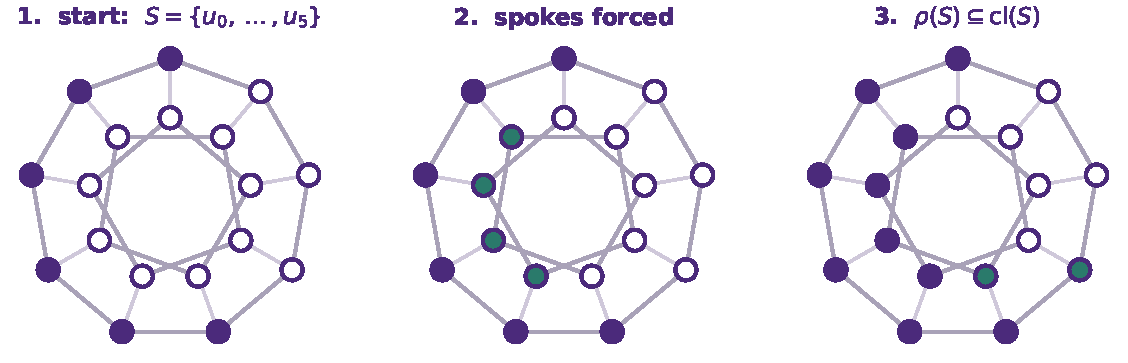
\includegraphics[width=0.75\textwidth]{figures/fig_forcing.pdf}
\caption{The Zero Forcing Colour Change Rule. A black vertex $u$ with exactly one white neighbour $w$ forces $w$ to become black ($u \to w$). If $u$ has two or more white neighbours, it is paralyzed and cannot force.}
\label{fig:forcing}
\end{figure}

\begin{defbox}{Definition 2.1: The Zero Forcing Rule}
Let $G = (V, E)$ be a simple, undirected graph. Initially, colour a chosen subset of vertices $S \subseteq V$ \textbf{black} (filled/active), and colour all remaining vertices $V \setminus S$ \textbf{white} (unfilled/inactive).
\begin{itemize}[leftmargin=*,nosep]
  \item \textbf{Colour Change Rule}: If a black vertex $u$ has \emph{exactly one} white neighbour $w \in N(u)$, then $w$ becomes black. We say that $u$ \textbf{forces} $w$, denoted $u \to w$.
  \item \textbf{Closure} $\operatorname{cl}(S)$: Apply the colour change rule iteratively until no further forces are possible. The final set of black vertices is the closure of $S$, denoted $\operatorname{cl}(S)$.
  \item \textbf{Zero Forcing Set}: If $\operatorname{cl}(S) = V$, then $S$ is called a \textbf{zero forcing set} of $G$.
  \item \textbf{Zero Forcing Number} $Z(G)$: The minimum cardinality of a zero forcing set:
  \begin{equation}
    Z(G) = \min \{ |S| \;\mid\; S \subseteq V, \, \operatorname{cl}(S) = V \}.
  \end{equation}
\end{itemize}
\end{defbox}

\begin{intubox}{Intuition \& High School Analogy: The Shy Rumour Speaker}
Imagine an epidemic or a rumour spreading across a high school:
\begin{itemize}[leftmargin=*,nosep]
  \item A student who knows the rumour is black; an uninformed student is white.
  \item The rule: A student who knows the rumour will only whisper it if there is \emph{exactly one person left} in their friendship group who hasn't heard it. If two or more friends haven't heard it, the speaker is paralyzed by indecision about whom to tell, so they say nothing.
  \item $Z(G)$ asks: What is the \emph{absolute minimum} number of students who must be seeded with the rumour initially so that eventually every single person in the school hears it?
\end{itemize}
\textbf{The paradox}: Counterintuitively, having \emph{more} black neighbours can make a vertex \emph{less} useful for future steps, because it only acts when its white neighbour count drops to exactly 1.
\end{intubox}

\begin{callbox}{Worked Numerical Example 2.1: Step-by-Step Zero Forcing Trace on a 4-Cycle $C_4$}
Let $G = C_4$ be the 4-cycle graph with vertices $V = \{1, 2, 3, 4\}$ and edges $E = \{(1,2), (2,3), (3,4), (4,1)\}$.
\begin{itemize}[leftmargin=*,nosep]
  \item \textbf{Trial 1: Can a single vertex force the graph ($|S|=1$)?}
  Try initial set $S = \{1\}$ (only vertex 1 is black).
  Look at vertex 1: its neighbours are $N(1) = \{2, 4\}$.
  Both neighbours are white. Since vertex 1 has 2 white neighbours, the colour change rule cannot fire.
  No other black vertices exist, so the process halts immediately:
  \begin{equation}
    \operatorname{cl}(\{1\}) = \{1\} \ne V \implies Z(C_4) > 1.
  \end{equation}
  \item \textbf{Trial 2: Two adjacent seed vertices ($S = \{1, 2\}$)}
  Start with $S = \{1, 2\}$ (vertices 1 and 2 are black, vertices 3 and 4 are white).
  \begin{itemize}[leftmargin=*,nosep]
    \item \textbf{Round 1}: Examine vertex 1. Its neighbours are vertex 2 (black) and vertex 4 (white).
    Vertex 1 has \emph{exactly one} white neighbour. Vertex 1 forces vertex 4:
    \begin{equation}
      1 \to 4 \implies \text{Black vertices: } \{1, 2, 4\}.
    \end{equation}
    \item \textbf{Round 2}: Examine vertex 2. Its neighbours are vertex 1 (black) and vertex 3 (white).
    Vertex 2 has \emph{exactly one} white neighbour. Vertex 2 forces vertex 3:
    \begin{equation}
      2 \to 3 \implies \text{Black vertices: } \{1, 2, 3, 4\} = V.
    \end{equation}
  \end{itemize}
  Every vertex is now black. Therefore $\operatorname{cl}(\{1, 2\}) = V$, proving:
  \begin{equation}
    Z(C_4) = 2.
  \end{equation}
\end{itemize}
\end{callbox}

\begin{defbox}{Fundamental Properties of the Closure Operator}
For any graph $G$ and vertex subsets $S, T \subseteq V$:
\begin{enumerate}[leftmargin=*,nosep]
  \item \textbf{Extensive}: $S \subseteq \operatorname{cl}(S)$.
  \item \textbf{Monotone}: If $S \subseteq T$, then $\operatorname{cl}(S) \subseteq \operatorname{cl}(T)$. (Starting with more seeds never yields fewer infected vertices.)
  \item \textbf{Idempotent}: $\operatorname{cl}(\operatorname{cl}(S)) = \operatorname{cl}(S)$. (Once the spreading process stops, restarting it changes nothing.)
  \item \textbf{Automorphism-Equivariant}: For any graph automorphism $\rho \in \operatorname{Aut}(G)$,
  \begin{equation}
    \rho(\operatorname{cl}(S)) = \operatorname{cl}(\rho(S)).
  \end{equation}
  (Rotating the graph first and then running zero forcing produces the exact same result as running zero forcing and then rotating.)
\end{enumerate}
\end{defbox}

\subsection{Maximum Nullity and Pattern Matrices}

\begin{defbox}{Definition 2.2: Pattern Classes and Maximum Nullity}
Let $G = (V, E)$ be a graph on $N$ vertices.
\begin{itemize}[leftmargin=*,nosep]
  \item \textbf{Symmetric Pattern Class} $S(G)$: The set of all real symmetric $N \times N$ matrices $A = A^T$ whose off-diagonal non-zero entries correspond precisely to the edges of $G$:
  \begin{equation}
    A_{uv} \ne 0 \iff uv \in E \qquad (u \ne v),
  \end{equation}
  while the diagonal entries $A_{uu}$ are completely free real numbers.
  \item \textbf{Combinatorially Symmetric Pattern Class} $S_{\mathrm{cs}}(G)$: The set of all real matrices $A$ (not necessarily symmetric) where:
  \begin{equation}
    A_{uv} \ne 0 \iff A_{vu} \ne 0 \iff uv \in E \qquad (u \ne v),
  \end{equation}
  with free diagonal entries. Clearly $S(G) \subseteq S_{\mathrm{cs}}(G)$.
  \item \textbf{Maximum Nullity} $M(G)$ and $M_{\mathrm{cs}}(G)$:
  \begin{equation}
    M(G) = \max_{A \in S(G)} \operatorname{null}(A), \qquad M_{\mathrm{cs}}(G) = \max_{A \in S_{\mathrm{cs}}(G)} \operatorname{null}(A).
  \end{equation}
  \item \textbf{Minimum Rank} $\operatorname{mr}(G) = N - M(G)$.
\end{itemize}
\end{defbox}

\subsection{The Fundamental Theorem: $M(G) \le M_{\mathrm{cs}}(G) \le Z(G)$}

\begin{thmbox}{Theorem 2.1: Maximum Nullity is Bounded by Zero Forcing}
For every graph $G$:
\begin{equation}
  M(G) \;\le\; M_{\mathrm{cs}}(G) \;\le\; Z(G).
\end{equation}
\end{thmbox}

\begin{defbox}{Rigorous Step-by-Step Proof}
Let $A \in S_{\mathrm{cs}}(G)$ be any matrix carrying the pattern of $G$. Let $S \subseteq V$ be any zero forcing set of $G$, so $|S| \ge Z(G)$.
Define the restriction linear map:
\begin{equation}
  \Phi_S : \ker(A) \to \mathbb{R}^{|S|}, \qquad \Phi_S(x) = x|_S.
\end{equation}
We claim that $\Phi_S$ is \textbf{injective}.
To prove injectivity, suppose $x \in \ker(A)$ satisfies $\Phi_S(x) = \mathbf{0}$, meaning $x_v = 0$ for all $v \in S$.
We prove by mathematical induction along the chronological zero forcing sequence that $x_w = 0$ for every forced vertex $w$.
\begin{itemize}[leftmargin=*,nosep]
  \item \textbf{Base case}: $x_v = 0$ for all $v \in S$.
  \item \textbf{Inductive step}: Suppose $x_v = 0$ for all currently black vertices $B \subseteq V$. Let $u \in B$ be an active black vertex with exactly one white neighbour $w \in V \setminus B$.
  Since $Ax = \mathbf{0}$, row $u$ of the matrix equation gives:
  \begin{equation}
    (Ax)_u = A_{uu} x_u + \sum_{v \in N(u)} A_{uv} x_v = 0.
  \end{equation}
  Split the sum over neighbours into the black neighbours and the single white neighbour $w$:
  \begin{equation}
    A_{uu} x_u + \sum_{v \in N(u) \cap B} A_{uv} x_v + A_{uw} x_w = 0.
  \end{equation}
  By the induction hypothesis, $x_u = 0$ and $x_v = 0$ for all $v \in N(u) \cap B$. Every term in the sum vanishes except the last:
  \begin{equation}
    0 + 0 + A_{uw} x_w = 0 \implies A_{uw} x_w = 0.
  \end{equation}
  Because $uw \in E$, the entry $A_{uw}$ is strictly non-zero ($A_{uw} \ne 0$). Therefore, we must have:
  \begin{equation}
    x_w = 0.
  \end{equation}
\end{itemize}
Because $S$ is a zero forcing set, the forcing sequence visits every vertex of $G$. Thus $x_v = 0$ for all $v \in V$, meaning $x = \mathbf{0}$.
Therefore, $\ker(\Phi_S) = \{\mathbf{0}\}$, so $\Phi_S$ is strictly injective.
By the Rank-Nullity Theorem applied to $\Phi_S$:
\begin{equation}
  \operatorname{null}(A) = \dim(\ker(A)) = \dim(\operatorname{im}(\Phi_S)) \le \dim(\mathbb{R}^{|S|}) = |S|.
\end{equation}
Since this inequality holds for every $A \in S_{\mathrm{cs}}(G)$ and every zero forcing set $S$, taking the maximum over $A$ and the minimum over $S$ yields:
\begin{equation}
  M(G) \le M_{\mathrm{cs}}(G) \le Z(G). \qedhere
\end{equation}
\end{defbox}

\begin{callbox}{High School Term-by-Term Dissection: The Asymmetry of Zero Forcing}
Notice the profound structural asymmetry between upper bounds and lower bounds:
\begin{itemize}[leftmargin=*,nosep]
  \item \textbf{Upper Bound on $Z(G)$}: Easy. To prove $Z(G) \le K$, you only need to \emph{exhibit a single set} $S$ of size $K$ and trace the colour change steps until the graph is filled.
  \item \textbf{Lower Bound on $Z(G)$}: Extremely difficult. To prove $Z(G) \ge K$, you must prove that \emph{no set of size $K-1$ can ever force the graph}. On a 60-vertex graph, testing all subsets of size 9 requires evaluating $\binom{60}{9} \approx 1.47 \times 10^{10}$ combinations.
  \item \textbf{The Matrix Miracle}: Theorem 2.1 gives us a backdoor. If we can construct \textbf{just one matrix} $A \in S(G)$ with nullity $K$, Theorem 2.1 guarantees:
  \begin{equation}
    Z(G) \ge M(G) \ge \operatorname{null}(A) = K.
  \end{equation}
  One single matrix certificate proves the lower bound for all $\binom{N}{K-1}$ sets simultaneously.
\end{itemize}
\end{callbox}

\begin{callbox}{Worked Numerical Example 2.2: Concrete Matrix Certificate Verifying $M(C_4) = Z(C_4) = 2$}
Consider the 4-cycle $C_4$. Let us construct an explicit symmetric pattern matrix $A \in S(C_4)$:
\begin{equation}
  A = \begin{pmatrix}
    0 & 1 & 0 & 1 \\
    1 & 0 & 1 & 0 \\
    0 & 1 & 0 & 1 \\
    1 & 0 & 1 & 0
  \end{pmatrix}.
\end{equation}
Notice that every off-diagonal non-zero matches an edge of $C_4$, so $A \in S(C_4)$.
Examine the rows:
\begin{itemize}[leftmargin=*,nosep]
  \item Row 1 and Row 3 are identical: $[0, 1, 0, 1]$.
  \item Row 2 and Row 4 are identical: $[1, 0, 1, 0]$.
\end{itemize}
Subtracting Row 1 from Row 3, and Row 2 from Row 4, produces two entire rows of zeros.
Thus, the row echelon form of $A$ has only 2 non-zero rows, meaning:
\begin{equation}
  \operatorname{rank}(A) = 2 \implies \operatorname{null}(A) = 4 - \operatorname{rank}(A) = 4 - 2 = \mathbf{2}.
\end{equation}
Solving $Ax = \mathbf{0}$ explicitly:
\begin{align}
  (Ax)_1 &= x_2 + x_4 = 0 \implies x_4 = -x_2, \\
  (Ax)_2 &= x_1 + x_3 = 0 \implies x_3 = -x_1.
\end{align}
The null space $\ker(A)$ is spanned by two linearly independent vectors:
\begin{equation}
  \ker(A) = \operatorname{span}\left\{
    v^{(1)} = \begin{pmatrix} 1 \\ 0 \\ -1 \\ 0 \end{pmatrix}, \quad
    v^{(2)} = \begin{pmatrix} 0 \\ 1 \\ 0 \\ -1 \end{pmatrix}
  \right\}.
\end{equation}
Now let us directly verify the injectivity of the restriction map $\Phi_S(x) = x|_S$ for our zero forcing set $S = \{1, 2\}$:
Suppose an arbitrary kernel vector $x = c_1 v^{(1)} + c_2 v^{(2)} = [c_1, \, c_2, \, -c_1, \, -c_2]^T$ vanishes on $S$:
\begin{equation}
  x_1 = c_1 = 0, \qquad x_2 = c_2 = 0.
\end{equation}
Then automatically $x_3 = -c_1 = 0$ and $x_4 = -c_2 = 0$, so $x = \mathbf{0}$.
Thus $\Phi_S$ is strictly injective, proving:
\begin{equation}
  \operatorname{null}(A) = 2 \le |S| = 2.
\end{equation}
Because $A \in S(C_4)$ has nullity 2, $M(C_4) \ge 2$. Combined with Theorem 2.1 and $Z(C_4)=2$:
\begin{equation}
  2 \le M(C_4) \le Z(C_4) = 2 \implies M(C_4) = Z(C_4) = 2. \qedhere
\end{equation}
\end{callbox}

\newpage

%% =========================================================================
%% SECTION 3: THE TARGET GRAPH FAMILIES
%% =========================================================================
\section{The Target Graph Families: Generalized Petersen Graphs and Cyclic Covers}

\subsection{Generalized Petersen Graphs $P(n,k)$}

\begin{defbox}{Definition 3.1: Generalized Petersen Graph $P(n,k)$}
Let $n \ge 3$ and $1 \le k < n/2$. The \textbf{Generalized Petersen graph} $P(n,k)$ has $2n$ vertices partitioned into:
\begin{itemize}[leftmargin=*,nosep]
  \item An \textbf{outer ring} $O = \{u_0, u_1, \dots, u_{n-1}\}$;
  \item An \textbf{inner ring} $I = \{v_0, v_1, \dots, v_{n-1}\}$.
\end{itemize}
The graph has $3n$ edges, defined for all $i \in \mathbb{Z}_n$ (indices modulo $n$):
\begin{equation}
  \underbrace{u_i u_{i+1}}_{\text{Outer Cycle Edges (Step 1)}}, \qquad
  \underbrace{u_i v_i}_{\text{Spoke Edges}}, \qquad
  \underbrace{v_i v_{i+k}}_{\text{Inner Jump Edges (Step } k)}.
\end{equation}
Every vertex touches exactly 3 edges, so $P(n,k)$ is cubic.
\end{defbox}

\begin{intubox}{Intuition \& High School Analogy: The Spoked Wheel}
Picture a bicycle wheel:
\begin{itemize}[leftmargin=*,nosep]
  \item The outer vertices $u_i$ form the outer tire (a simple circle of circumference $n$).
  \item The spokes $u_i v_i$ run radially inward to the hub.
  \item But the hub $v_i$ is not a simple circle: each inner node connects to the node $k$ positions ahead.
  \item By the Clock Orbit Lemma (Theorem 1.1), the inner vertices decompose into exactly $d = \gcd(n,k)$ separate star-polygons or cycles.
  \item For $n=5, k=2$, $P(5,2)$ is the famous \textbf{Petersen Graph}, first discovered in 1898 as a counterexample to Tait's four-colour conjecture.
\end{itemize}
\end{intubox}

\subsection{$I$-Graphs $I(n,j,k)$}

\begin{defbox}{Definition 3.2: The $I$-Graph $I(n,j,k)$}
The \textbf{$I$-graph} $I(n,j,k)$ generalizes $P(n,k)$ by allowing the outer ring to also make jumps of step $j$:
\begin{equation}
  \text{Outer: } u_i u_{i+j}, \qquad \text{Spokes: } u_i v_i, \qquad \text{Inner: } v_i v_{i+k}, \qquad (i \in \mathbb{Z}_n).
\end{equation}
Notice that $P(n,k) = I(n,1,k)$.
The outer edges decompose into $d_1 = \gcd(n,j)$ cycles, while the inner edges decompose into $d_2 = \gcd(n,k)$ cycles.
\end{defbox}

\begin{thmbox}{Theorem 3.1: Reduction of $I$-Graphs to Generalized Petersen Graphs}
If $\gcd(n, j) = 1$, then $j$ has a multiplicative modular inverse $j^{-1} \pmod n$. 
The map $\psi(u_i) = u_{j \cdot i \bmod n}$ and $\psi(v_i) = v_{j \cdot i \bmod n}$ is an exact graph isomorphism:
\begin{equation}
  I(n, j, k) \;\cong\; I(n, 1, j^{-1}k \bmod n) \;=\; P(n, j^{-1}k \bmod n).
\end{equation}
\end{thmbox}

\begin{callbox}{Scope of Genuine $I$-Graph Invariants}
Theorem 3.1 demonstrates that whenever $\gcd(n,j)=1$, the $I$-graph is secretly just a Generalized Petersen graph in disguise. 
Therefore, genuinely new mathematical behavior in $I(n,j,k)$ only exists when:
\begin{equation}
  \gcd(n, j) > 1 \qquad \text{and} \qquad \gcd(n, k) > 1.
\end{equation}
\end{callbox}

\subsection{Double Generalized Petersen Graphs $DP(n,k)$}

\begin{defbox}{Definition 3.3: Double Generalized Petersen Graph $DP(n,k)$}
The graph $DP(n,k)$ has $4n$ vertices partitioned into four rings of size $n$: two outer cycles $\{u_i\}, \{x_i\}$ and two inner rings $\{w_i\}, \{y_i\}$. The edges are:
\begin{align}
  \text{Outer 1: } & u_i u_{i+1}, & \text{Outer 2: } & x_i x_{i+1}, \\
  \text{Spokes 1: } & u_i w_i, & \text{Spokes 2: } & x_i y_i, \\
  \text{Cross-Inner: } & w_i y_{i+k}, \quad y_i w_{i+k}.
\end{align}
$DP(n,k)$ is a bipartite cubic graph on $4n$ vertices studied in topological graph theory for its extremal symmetry and Hamiltonicity.
\end{defbox}

\subsection{Cyclic Covers of Graphs (Topological Graph Theory)}

\begin{defbox}{Definition 3.4: Voltage Graphs and Derived Covers}
Let $B = (V_B, E_B)$ be a small finite multigraph called the \textbf{base graph}. Assign to each directed edge $e = (x, y) \in E_B$ an element $\alpha(e) \in \mathbb{Z}_n$, called its \textbf{voltage}.
The \textbf{derived cyclic cover} $B^n$ is the graph with:
\begin{itemize}[leftmargin=*,nosep]
  \item Vertex set $V(B^n) = V_B \times \mathbb{Z}_n$. For each base vertex $x \in V_B$, the set $\{ (x, i) \mid i \in \mathbb{Z}_n \}$ is called the \textbf{fiber} above $x$.
  \item Edge set: For every edge $e = (x, y) \in E_B$ with voltage $\alpha(e) = v$, connect $(x, i)$ to $(y, i + v \pmod n)$ for all $i \in \mathbb{Z}_n$.
\end{itemize}
\end{defbox}

\begin{intubox}{Intuition: $P(n,k)$ is a 2-Vertex Voltage Cover.}
How do we view $P(n,k)$ as a cyclic cover?
Take a base graph $B$ with just \textbf{two vertices}: $u$ (outer) and $v$ (inner).
\begin{itemize}[leftmargin=*,nosep]
  \item Put a self-loop at $u$ with voltage $+1$. (When lifted to $n$ levels, this creates the outer cycle $u_i u_{i+1}$.)
  \item Put a self-loop at $v$ with voltage $+k$. (When lifted, this creates the inner chords $v_i v_{i+k}$.)
  \item Put a spoke edge connecting $u$ and $v$ with voltage $0$. (When lifted, this connects $(u, i)$ to $(v, i)$.)
\end{itemize}
Thus, Generalized Petersen graphs are simply the $n$-fold cyclic covers of a two-vertex base graph. All theorems derived in this project naturally generalize to arbitrary cyclic covers of any base graph.
\end{intubox}

\newpage

%% =========================================================================
%% SECTION 4: UPPER BOUNDS VIA THE ROTATION BOOTSTRAP
%% =========================================================================
\section{Upper Bounds: The Rotation-Bootstrap Method}

How do we prove upper bounds like $Z(P(n,k)) \le 2k+2$ for \emph{every single $n$} simultaneously without having to analyze an infinite number of graphs one by one?
The solution is the \textbf{Rotation Bootstrap}, a powerful mathematical technique introduced in this project that converts a finite 3-step hand check into a universal theorem valid for all $n$.

\subsection{The Fundamental Bootstrap Lemmas}

\begin{thmbox}{Lemma 4.1: The Rotation-Bootstrap Lemma}
Let $G = (V, E)$ be a finite graph, and let $\rho \in \operatorname{Aut}(G)$ be an automorphism of $G$. 
If a vertex subset $S \subseteq V$ satisfies
\begin{equation}
  \rho(S) \subseteq \operatorname{cl}(S),
\end{equation}
then the closure $\operatorname{cl}(S)$ is strictly invariant under rotation:
\begin{equation}
  \rho(\operatorname{cl}(S)) = \operatorname{cl}(S).
\end{equation}
\end{thmbox}

\begin{defbox}{Line-by-Line Algebraic Proof}
We apply the four closure properties established in Section 2:
\begin{align}
  \rho(\operatorname{cl}(S)) &= \operatorname{cl}(\rho(S)) && \text{(Closure commutes with automorphisms)} \label{eq:boot1}\\
  &\subseteq \operatorname{cl}(\operatorname{cl}(S)) && \text{(Since } \rho(S) \subseteq \operatorname{cl}(S) \text{ and closure is monotone)} \label{eq:boot2}\\
  &= \operatorname{cl}(S) && \text{(Closure is idempotent: } \operatorname{cl}(\operatorname{cl}(X)) = \operatorname{cl}(X)\text{)}. \label{eq:boot3}
\end{align}
Eq.~\eqref{eq:boot3} establishes that $\rho(\operatorname{cl}(S)) \subseteq \operatorname{cl}(S)$.
Now consider the cardinalities. Because $\rho$ is an automorphism (a bijective permutation of the finite vertex set $V$), applying $\rho$ to any subset preserves its exact number of elements:
\begin{equation}
  |\rho(\operatorname{cl}(S))| = |\operatorname{cl}(S)|.
\end{equation}
If a finite set $A$ is a subset of $B$ and $|A| = |B|$, then $A$ must equal $B$ identically.
Therefore:
\begin{equation}
  \rho(\operatorname{cl}(S)) = \operatorname{cl}(S). \qedhere
\end{equation}
\end{defbox}

\begin{intubox}{Intuition \& High School Analogy: The Domino Wheel}
Think of standing dominoes around a giant circular track:
\begin{itemize}[leftmargin=*,nosep]
  \item If your starting push can topple the first block and successfully reach \emph{one position past where you started} ($\rho(S)$), the system has replicated its own initial conditions shifted by one notch.
  \item By rotational symmetry, the shifted configuration will topple the next notch, which topples the next notch, which topples the next notch..
  \item The chain reaction can never stop until the entire circular wheel is knocked down.
\end{itemize}
\end{intubox}

\begin{thmbox}{Lemma 4.2: The Closing Lemma for Spoke Graphs}
Let $G$ be a cubic graph whose vertex set partitions into an outer ring $O$ and an inner ring $I$ such that:
\begin{enumerate}[leftmargin=*,nosep]
  \item Every vertex of $O$ has exactly one neighbour in $I$ (its spoke), and its other two neighbours lie in $O$.
  \item Every vertex of $I$ has exactly one neighbour in $O$.
\end{enumerate}
If $O \subseteq \operatorname{cl}(S)$, then $\operatorname{cl}(S) = V(G)$.
\end{thmbox}

\begin{defbox}{Proof}
Assume $O \subseteq \operatorname{cl}(S)$, so every outer vertex is black. 
Suppose there exists an unfilled white vertex $w \in I$. By condition (2), $w$ has a unique neighbour $o \in O$.
Now examine vertex $o$:
\begin{itemize}[leftmargin=*,nosep]
  \item $o$ is black (since $o \in O \subseteq \operatorname{cl}(S)$).
  \item The degree of $o$ is 3. Its two other neighbours lie in $O$, so both are already black.
  \item Its third neighbour is $w$, which is white.
\end{itemize}
Therefore, black vertex $o$ has \emph{exactly one white neighbour}, namely $w$. By the colour change rule, $o$ forces $w$ to turn black.
Since this holds for every $w \in I$, no white vertex can survive. Thus $\operatorname{cl}(S) = V(G)$. \qedhere
\end{defbox}

\subsection{The Unified Upper Bound for $I$-Graphs}

\begin{figure}[htbp]
\centering
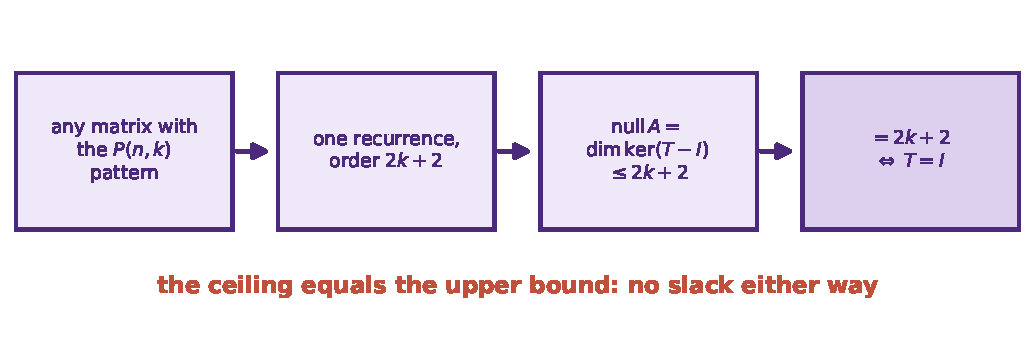
\includegraphics[width=0.95\textwidth]{figures/fig_chain.pdf}
\caption{The 3-Step Rotation-Bootstrap Forcing Chain for $I(n,j,k)$. Step 1: Outer vertices $u_i$ force spoke neighbours $v_i$. Step 2: Inner vertex $v_{j+k}$ forces $v_{j+2k}$ across the jump chord. Step 3: Outer vertex $u_{j+2k}$ forces $u_{2(j+k)}$, completing the shift $\rho(S)$.}
\label{fig:chain}
\end{figure}

\begin{thmbox}{Theorem 4.1: Unified Upper Bound for $I(n,j,k)$}
For all integers $j \ge 1$, $k \ge 1$, and all $n \ge 2(j+k) + 1$:
\begin{equation}
  Z(I(n, j, k)) \;\le\; 2(j+k).
\end{equation}
\end{thmbox}

\begin{defbox}{Rigorous Proof via the 3-Step Forcing Chain}
Let $m = 2(j+k)$, and choose the seed set to be $m$ consecutive outer vertices:
\begin{equation}
  S = \{ u_0, u_1, u_2, \dots, u_{m-1} \}.
\end{equation}
Since $n \ge m + 1$, the indices $0, 1, \dots, m$ are strictly distinct modulo $n$.
We execute a deterministic 3-step forcing chain:

\noindent\textbf{Step 1: Outer vertices force their spokes.}
Consider an outer vertex $u_i$. Its three neighbours are $u_{i-j}$, $u_{i+j}$, and $v_i$.
Both outer neighbours $u_{i-j}$ and $u_{i+j}$ belong to $S = \{u_0, \dots, u_{m-1}\}$ if and only if:
\begin{equation}
  i - j \ge 0 \quad \text{and} \quad i + j \le m - 1 \iff j \le i \le m - 1 - j.
\end{equation}
For every such $i$, $u_i$ is black and both its outer neighbours are black. Its only remaining neighbour is spoke $v_i$ (white).
Thus, $u_i \to v_i$ forces spoke $v_i$ for all $i \in \{j, j+1, \dots, m - 1 - j\}$.
Since $m = 2(j+k)$, the upper index is $2(j+k) - 1 - j = j + 2k - 1$.
Therefore, Step 1 fills the contiguous inner block:
\begin{equation}
  V_{\text{Step 1}} = \{ v_j, v_{j+1}, \dots, v_{j+2k-1} \}.
\end{equation}

\noindent\textbf{Step 2: An inner vertex reaches forward across the chords.}
Now examine the inner vertex $v_{j+k}$. Its three neighbours are:
\begin{enumerate}[leftmargin=*,nosep]
  \item $u_{j+k} \in S$ (since $j+k \le 2(j+k)-1 = m-1$, black);
  \item $v_{(j+k)-k} = v_j$ (which was filled in Step 1, black);
  \item $v_{(j+k)+k} = v_{j+2k}$ (which was \textbf{not} filled in Step 1, because Step 1 stopped at index $j+2k-1$.).
\end{enumerate}
Therefore, black vertex $v_{j+k}$ has exactly one white neighbour: $v_{j+2k}$.
By the colour change rule, $v_{j+k} \to v_{j+2k}$ forces $v_{j+2k}$ black.

\noindent\textbf{Step 3: The inner chord forces back out to the next outer vertex.}
Now examine the outer vertex $u_{j+2k} = u_{m-j}$. Its three neighbours are:
\begin{enumerate}[leftmargin=*,nosep]
  \item $u_{(j+2k)-j} = u_{2k} \in S$ (since $2k \le 2(j+k)-1$, black);
  \item Spoke $v_{j+2k}$ (which was just forced black in Step 2.);
  \item $u_{(j+2k)+j} = u_{j+2k+j} = u_{2j+2k} = u_m$ (which is white, as $S$ only goes up to $m-1$).
\end{enumerate}
Therefore, black vertex $u_{j+2k}$ has exactly one white neighbour: $u_m$.
By the colour change rule, $u_{j+2k} \to u_m$ forces $u_m$ black.

\noindent\textbf{Conclusion via Bootstrap and Closing:}
We started with $S = \{u_0, u_1, \dots, u_{m-1}\}$. We have now forced $u_m$.
Thus, the closure contains:
\begin{equation}
  \{u_1, u_2, \dots, u_m\} = \rho(S) \subseteq \operatorname{cl}(S).
\end{equation}
By the Rotation-Bootstrap Lemma (Lemma 4.1), $\operatorname{cl}(S)$ is rotation-invariant.
Since $u_0 \in \operatorname{cl}(S)$, rotating $u_0$ by $\rho$ repeatedly generates all $n$ outer vertices:
\begin{equation}
  O = \{u_0, u_1, \dots, u_{n-1}\} \subseteq \operatorname{cl}(S).
\end{equation}
Finally, by the Closing Lemma (Lemma 4.2), since the entire outer ring is filled, every inner vertex is forced by its outer spoke.
Thus $\operatorname{cl}(S) = V(I(n, j, k))$, which proves $Z(I(n, j, k)) \le |S| = 2(j+k)$. \qedhere
\end{defbox}

\begin{callbox}{Why is $m = 2(j+k)$ Exact?}
Look closely at the index arithmetic in Step 2:
\begin{itemize}[leftmargin=*,nosep]
  \item Vertex $v_{m-j-k}$ looks backward to $v_{m-j-2k}$.
  \item For Step 2 to work, $v_{m-j-2k}$ must already be black from Step 1.
  \item The very first vertex filled in Step 1 is $v_j$.
  \item Setting them equal: $m - j - 2k = j \iff m = 2(j+k)$.
\end{itemize}
$m = 2(j+k)$ is not an empirical guess: it is the \emph{unique algebraic integer} where the forward and backward index chains mesh perfectly.
\end{callbox}

\begin{callbox}{Worked Numerical Example 4.1: Hand-Tracing the Full Rotation Bootstrap on $P(7,2)$}
Let us execute the exact forcing steps on $P(7,2)$ ($j=1, k=2, n=7$). 
The threshold formula gives $m = 2(j+k) = 2(1+2) = 6$, and $n = 7 \ge 2(1+2)+1 = 7$ (exactly tight.).
Start with seed set of $m=6$ outer vertices:
\begin{equation}
  S = \{u_0, u_1, u_2, u_3, u_4, u_5\}.
\end{equation}
Initially, only $u_6$ on the outer ring is white, and all inner vertices $\{v_0, \dots, v_6\}$ are white.
\begin{itemize}[leftmargin=*,nosep]
  \item \textbf{Step 1: Outer forces spokes}:
  \begin{itemize}[leftmargin=*,nosep]
    \item Vertex $u_1$: neighbours are $u_0$ (black), $u_2$ (black), and spoke $v_1$ (white) $\implies \mathbf{u_1 \to v_1}$.
    \item Vertex $u_2$: neighbours are $u_1$ (black), $u_3$ (black), and spoke $v_2$ (white) $\implies \mathbf{u_2 \to v_2}$.
    \item Vertex $u_3$: neighbours are $u_2$ (black), $u_4$ (black), and spoke $v_3$ (white) $\implies \mathbf{u_3 \to v_3}$.
    \item Vertex $u_4$: neighbours are $u_3$ (black), $u_5$ (black), and spoke $v_4$ (white) $\implies \mathbf{u_4 \to v_4}$.
  \end{itemize}
  Black set after Step 1: $S \cup \{v_1, v_2, v_3, v_4\}$.
  \item \textbf{Step 2: Inner reaches forward}:
  Look at inner vertex $v_3$ ($j+k = 1+2 = 3$). Its three neighbours are:
  \begin{enumerate}[leftmargin=*,nosep]
    \item Spoke $u_3 \in S$ (black);
    \item Backward chord $v_{3-2} = v_1$ (black, from Step 1);
    \item Forward chord $v_{3+2} = v_5$ (\textbf{white}.).
  \end{enumerate}
  Vertex $v_3$ has \emph{exactly one white neighbour}. Thus $\mathbf{v_3 \to v_5}$ forces $v_5$ black.
  \item \textbf{Step 3: Spokes force out to advance the outer wave}:
  Look at outer vertex $u_5$ ($j+2k = 1+4 = 5$). Its three neighbours are:
  \begin{enumerate}[leftmargin=*,nosep]
    \item Backward outer neighbour $u_4 \in S$ (black);
    \item Spoke neighbour $v_5$ (black, just forced in Step 2.);
    \item Forward outer neighbour $u_6$ (\textbf{white}.).
  \end{enumerate}
  Vertex $u_5$ has \emph{exactly one white neighbour}. Thus $\mathbf{u_5 \to u_6}$ forces $u_6$ black.
\end{itemize}
We now have $\{u_1, u_2, u_3, u_4, u_5, u_6\} = \rho(S) \subseteq \operatorname{cl}(S)$.
By Lemma 4.1, $\operatorname{cl}(S)$ is rotation-invariant, so it contains all 7 outer vertices: $O = \{u_0, \dots, u_6\} \subseteq \operatorname{cl}(S)$.
Finally, every outer vertex $u_i$ is black and touches two black outer neighbours, so $u_0 \to v_0$ and $u_6 \to v_6$ force the remaining spokes.
The entire 14-vertex graph is black, proving $Z(P(7,2)) \le 6 = 2k+2$.
\end{callbox}

\subsection{Corollaries and Bounds for $P(n,k)$ and $DP(n,k)$}

\begin{thmbox}{Corollary 4.2: Upper Bound for Generalized Petersen Graphs}
For all $k \ge 1$ and $n \ge 2k+3$:
\begin{equation}
  Z(P(n, k)) \;\le\; 2k + 2.
\end{equation}
\end{thmbox}
\begin{defbox}{Proof}
$P(n,k) = I(n, 1, k)$. Set $j=1$ in Theorem 4.1: $2(j+k) = 2(1+k) = 2k+2$. \qedhere
\end{defbox}

\begin{thmbox}{Theorem 4.3: Upper Bound for Double Generalized Petersen Graphs}
For all $k \ge 1$ and $n \ge 2k+3$:
\begin{equation}
  Z(DP(n, k)) \;\le\; 4k + 4.
\end{equation}
\end{thmbox}
\begin{defbox}{Proof Idea}
Choose $S = \{u_0, \dots, u_{2k+1}\} \cup \{x_0, \dots, x_{2k+1}\}$, of size $4k+4$. Run the 3-step forcing chain simultaneously on both outer rails $u$ and $x$. The cross-inner edges $w_i y_{i+k}$ and $y_i w_{i+k}$ exchange information symmetrically, forcing $u_{2k+2}$ and $x_{2k+2}$, which yields $\rho(S) \subseteq \operatorname{cl}(S)$ and closes the entire $4n$-vertex complex. \qedhere
\end{defbox}

\subsection{The False Published Literature and the Quest for Sharpness}

\begin{callbox}{Historical Context: The False 2020 Theorem and the July 2026 Crisis}
In 2020, Rashidi, Shajareh Poursalavati, and Tavakkoli published a paper claiming that $Z(P(n,3)) = 8$ for all $n \ge 12$.
\begin{itemize}[leftmargin=*,nosep]
  \item \textbf{The Disaster}: In July 2026, A.~Krishnan published an arXiv correction note (arXiv:2607.19412) proving that Theorem 3.6 of Rashidi et al.\ is \textbf{flatly false}: for $n=12$, $Z(P(12,3)) = 7 \ne 8$. The authors had made a case-analysis error that failed to test 7-vertex sets.
  \item \textbf{The Open Problem}: Krishnan's note concluded with the open challenge:
  \begin{center}
    \emph{``Determining $Z(P(n,k))$ for general $k$ --- the stabilization threshold and a rigorous lower bound for $k \ge 4$ --- remains completely open.''}
  \end{center}
\end{itemize}
\end{callbox}

\begin{figure}[htbp]
\centering
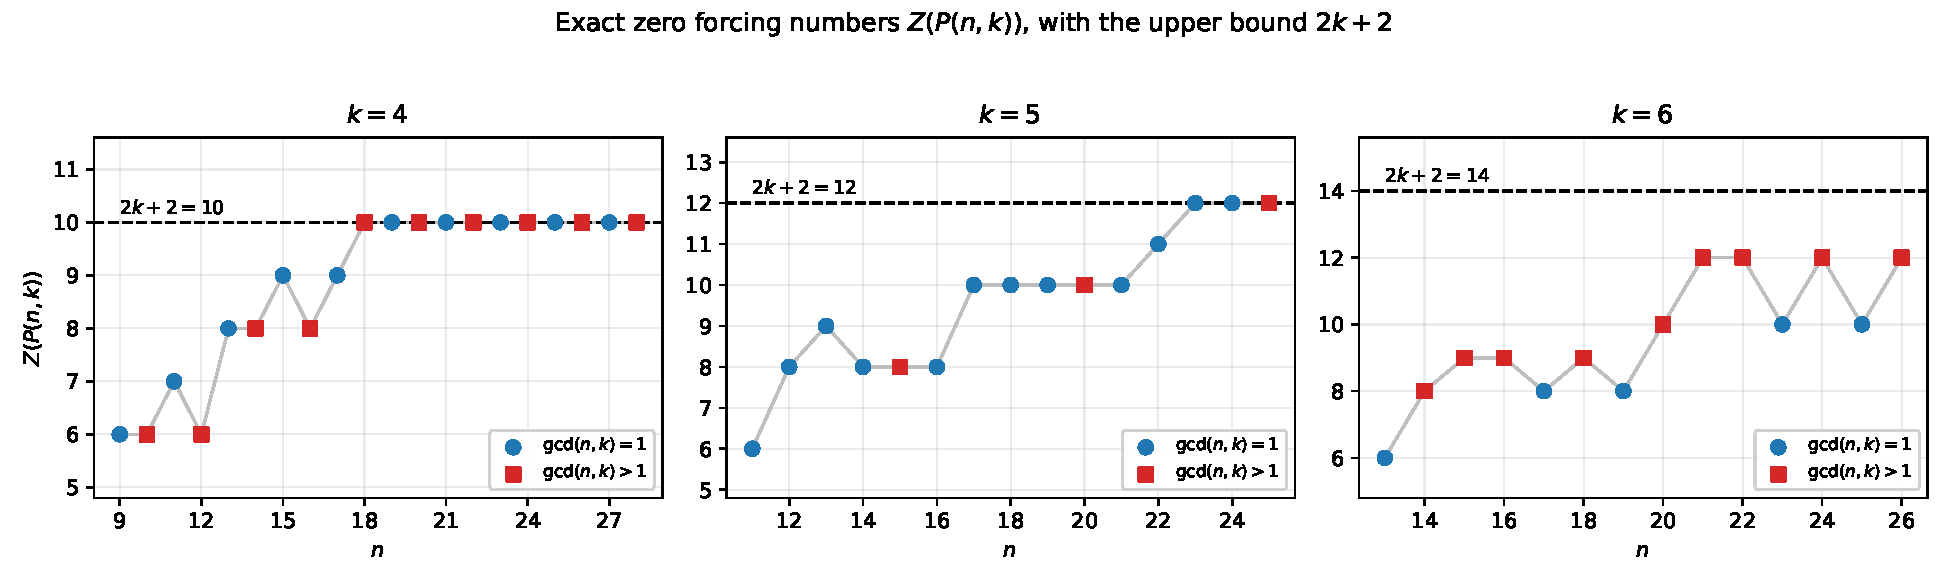
\includegraphics[width=0.92\textwidth]{figures/zf_sequences.pdf}
\caption{Exact zero forcing numbers $Z(P(n,k))$ for $k=4, 5, 6$ as a function of $n$. Notice the striking non-monotonicity: $k=4$ dips at $n=12, 16$; $k=6$ attains $14$ at $n=28$ but drops back to $12$ at $n=29$.}
\label{fig:sequences}
\end{figure}

\newpage

%% =========================================================================
%% SECTION 5: WHY COMBINATORIAL LOWER BOUNDS FAIL
%% =========================================================================
\section{The Lower Bound Impasse: Why Combinatorial Methods Fail}

Before developing our algebraic matrix certificate method, we rigorously demonstrate why all standard combinatorial techniques in graph theory fail to prove lower bounds for $Z(P(n,k))$.

\subsection{Forts and Fort Duality}

\begin{defbox}{Definition 5.1: Fort}
A non-empty vertex subset $F \subseteq V$ is called a \textbf{fort} if every vertex $w \notin F$ outside the fort has either $0$ or at least $2$ neighbours in $F$:
\begin{equation}
  |N(w) \cap F| \ne 1 \qquad \forall w \in V \setminus F.
\end{equation}
\end{defbox}

\begin{intubox}{Intuition: The Impenetrable Fortress}
Imagine $F$ is entirely white (uninfected). Can any black vertex outside $F$ force a vertex inside $F$?
\begin{itemize}[leftmargin=*,nosep]
  \item To force, an outside vertex $w$ must have \emph{exactly one} white neighbour.
  \item But if $w$ has neighbours in $F$, the fort definition says it must have \emph{at least 2} neighbours in $F$.
  \item Since both are white, $w$ has $\ge 2$ white neighbours, paralyzing it.
  \item Therefore, \textbf{an unseeded fort can never be penetrated}: it stays white forever.
\end{itemize}
\end{intubox}

\begin{thmbox}{Theorem 5.1: Fort Duality (Zero Forcing as a Hitting Set)}
A vertex subset $S \subseteq V$ is a zero forcing set of $G$ if and only if $S$ intersects (hits) every fort of $G$:
\begin{equation}
  S \cap F \ne \emptyset \qquad \forall \text{ forts } F \subseteq V.
\end{equation}
Consequently, $Z(G)$ equals the \textbf{minimum hitting set} of the hypergraph of forts.
\end{thmbox}

\subsection{The Three Combinatorial Failures}

\begin{callbox}{Failure Mode 1: Disjoint Fort Packing}
If a graph contains $t$ pairwise disjoint forts $F_1, F_2, \dots, F_t$ ($F_i \cap F_j = \emptyset$), then any hitting set must pick at least one distinct vertex from each fort, proving $Z(G) \ge t$.
\begin{itemize}[leftmargin=*,nosep]
  \item \textbf{Why it fails on $P(n,k)$}: Exhaustive computation reveals that every fort in $P(n,k)$ is massive, containing between $7$ and $13$ vertices.
  \item In a graph with $2n \le 56$ vertices, at most \textbf{two} disjoint forts can ever fit geometrically.
  \item The disjoint fort packing bound gives:
  \begin{equation}
    Z(P(n,k)) \ge 2.
  \end{equation}
  This is completely useless when the true value is $Z = 10, 12, 14$.
\end{itemize}
\end{callbox}

\begin{callbox}{Failure Mode 2: Linear Programming (LP) Relaxation}
The minimum hitting set problem can be formulated as an integer linear program (ILP):
\begin{equation}
  \min \sum_{v \in V} x_v \quad \text{subject to} \quad \sum_{v \in F} x_v \ge 1 \; (\forall F), \quad x_v \in \{0, 1\}.
\end{equation}
Relaxing $x_v \in [0, 1]$ gives the fractional hitting set LP value $\mathrm{LP}(G) \le Z(G)$.
\begin{itemize}[leftmargin=*,nosep]
  \item \textbf{The measured integrality gap}: Computing the exact LP value via cutting planes reveals:
  \begin{equation}
    \frac{\mathrm{LP}(P(n,k))}{Z(P(n,k))} \approx 0.43 - 0.50.
  \end{equation}
  For example, on $P(12,3)$, $\mathrm{LP} = 3.00$ while $Z = 7$. On $P(18,4)$, $\mathrm{LP} = 3.21$ while $Z = 10$.
  \item The integrality gap is a massive factor of $2$ and \emph{widens as $k$ increases}.
  \item This explains why branch-and-bound ILP solvers stall completely: they must close a factor-of-2 gap by pure exponential tree branching.
\end{itemize}
\end{callbox}

\begin{callbox}{Failure Mode 3: Hoffman-Type Spectral Bounds}
Spectral graph theory offers ratio bounds using the smallest adjacency eigenvalue $\lambda_{\min}$:
\begin{equation}
  Z(G) \ge N \left( 1 + \frac{2\lambda_{\min}}{3 - \lambda_{\min}} \right).
\end{equation}
\begin{itemize}[leftmargin=*,nosep]
  \item On $P(n,k)$, this formula yields lower bounds between $1.2$ and $2.9$.
  \item As $k$ grows, the bound further degrades, providing zero useful information.
\end{itemize}
\end{callbox}

\noindent
\textbf{The Conclusion}: All combinatorial and graph-theoretic techniques fail in principle, not merely in practice. To conquer lower bounds, we must switch mathematical categories entirely and move to \textbf{algebraic matrix certificates}.

\newpage

%% =========================================================================
%% SECTION 6: MONODROMY, RECURRENCES, & THE EXACT CEILING
%% =========================================================================
\section{Monodromy, Recurrences, and the Exact Ceiling}

\subsection{The Matrix Pattern Formulation}

Let $A$ be \emph{any} real matrix (symmetric or combinatorially symmetric) carrying the edge pattern of $P(n,k)$. Label its non-zero entries:
\begin{itemize}[leftmargin=*,nosep]
  \item Outer forward edge: $A_{u_i u_{i+1}} = b_i \ne 0$; Outer backward edge: $A_{u_{i+1} u_i} = b'_i \ne 0$.
  \item Spoke inward edge: $A_{u_i v_i} = c_i \ne 0$; Spoke outward edge: $A_{v_i u_i} = c'_i \ne 0$.
  \item Inner forward edge: $A_{v_i v_{i+k}} = e_i \ne 0$; Inner backward edge: $A_{v_{i+k} v_i} = e'_i \ne 0$.
  \item Outer diagonal: $A_{u_i u_i} = a_i$; Inner diagonal: $A_{v_i v_i} = d_i$.
\end{itemize}
For a symmetric matrix, $b'_i = b_i$, $c'_i = c_i$, and $e'_i = e_i$.

\subsection{The Inner Elimination Theorem: Derivation of the 9-Term Recurrence}

\begin{figure}[htbp]
\centering
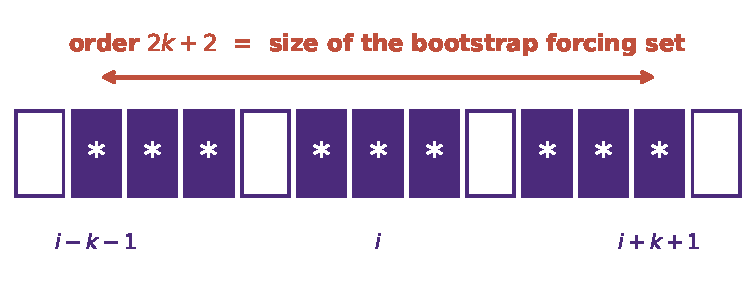
\includegraphics[width=0.92\textwidth]{figures/fig_recurrence.pdf}
\caption{The 9-Term Recurrence Stencil. Row $u_i$ expresses the inner hub variable $y_i$ in terms of outer neighbours $x_{i-1}, x_i, x_{i+1}$. Substituting into row $v_i$ connects three staggered triplets, yielding a 9-term linear relation of order exactly $2k+2$.}
\label{fig:recurrence}
\end{figure}

\begin{thmbox}{Theorem 6.1: Inner Elimination and the Monodromy Recurrence}
Let $n > 2k$. Any kernel vector $\begin{pmatrix} x \\ y \end{pmatrix} \in \ker(A)$ (where $x \in \mathbb{R}^n$ represents outer vertices and $y \in \mathbb{R}^n$ represents inner vertices) is uniquely determined by $x$, where $x$ satisfies a \textbf{9-term linear recurrence relation of order exactly $2k+2$}:
\begin{equation}
  \sum_{p=-k-1}^{k+1} \gamma_{i,p} \, x_{i+p} = 0 \qquad \forall i \in \mathbb{Z}_n.
\end{equation}
The extreme coefficients are strictly non-zero:
\begin{equation}
  \gamma_{i, k+1} = -\frac{e_i b_{i+k}}{c_{i+k}} \ne 0, \qquad \gamma_{i, -k-1} = -\frac{e'_{i-k} b'_{i-k-1}}{c_{i-k}} \ne 0.
\end{equation}
\end{thmbox}

\begin{defbox}{Step-by-Step Algebraic Derivation}
\noindent\textbf{Step 1: Express inner variables $y$ in terms of outer variables $x$.}
Examine row $u_i$ of the homogeneous system $A \begin{pmatrix} x \\ y \end{pmatrix} = \mathbf{0}$:
\begin{equation}
  (Ax)_{u_i} = b'_{i-1} x_{i-1} + a_i x_i + b_i x_{i+1} + c_i y_i = 0.
\end{equation}
Because the spoke weight $c_i \ne 0$, we can divide by $c_i$ to solve for $y_i$ uniquely:
\begin{equation}
  y_i = (Lx)_i = -\frac{b'_{i-1} x_{i-1} + a_i x_i + b_i x_{i+1}}{c_i}. \label{eq:y_elim}
\end{equation}
This eliminates all $n$ inner variables in terms of 3-term windows of outer variables.

\noindent\textbf{Step 2: Substitute $y$ into the inner row equations.}
Now examine row $v_i$ of the system $A \begin{pmatrix} x \\ y \end{pmatrix} = \mathbf{0}$:
\begin{equation}
  (Ay)_{v_i} = e'_{i-k} y_{i-k} + d_i y_i + e_i y_{i+k} + c'_i x_i = 0. \label{eq:v_row}
\end{equation}
Substitute Eq.~\eqref{eq:y_elim} into Eq.~\eqref{eq:v_row} for the three terms $y_{i-k}$, $y_i$, and $y_{i+k}$:
\begin{align}
  -e'_{i-k} &\left( \frac{b'_{i-k-1} x_{i-k-1} + a_{i-k} x_{i-k} + b_{i-k} x_{i-k+1}}{c_{i-k}} \right) \nonumber \\
  -d_i &\left( \frac{b'_{i-1} x_{i-1} + a_i x_i + b_i x_{i+1}}{c_i} \right) \nonumber \\
  -e_i &\left( \frac{b'_{i+k-1} x_{i+k-1} + a_{i+k} x_{i+k} + b_{i+k} x_{i+k+1}}{c_{i+k}} \right) + c'_i x_i = 0. \label{eq:full_recurrence}
\end{align}

\noindent\textbf{Step 3: Analyze the index support.}
Look at the outer indices appearing in Eq.~\eqref{eq:full_recurrence}:
\begin{itemize}[leftmargin=*,nosep]
  \item First term ($y_{i-k}$): indices $\{ i-k-1, \; i-k, \; i-k+1 \}$;
  \item Second term ($y_i$): indices $\{ i-1, \; i, \; i+1 \}$;
  \item Third term ($y_{i+k}$): indices $\{ i+k-1, \; i+k, \; i+k+1 \}$.
\end{itemize}
These form exactly 9 index positions centered at $i$.
The highest index is $i + k + 1$, whose coefficient is:
\begin{equation}
  \gamma_{i, k+1} = -\frac{e_i b_{i+k}}{c_{i+k}}.
\end{equation}
Since $e_i \ne 0$ and $b_{i+k} \ne 0$, $\gamma_{i, k+1} \ne 0$.
The lowest index is $i - k - 1$, whose coefficient is:
\begin{equation}
  \gamma_{i, -k-1} = -\frac{e'_{i-k} b'_{i-k-1}}{c_{i-k}} \ne 0.
\end{equation}
The total span of the recurrence is:
\begin{equation}
  \text{Order} = (i + k + 1) - (i - k - 1) = 2k + 2. \qedhere
\end{equation}
\end{defbox}

\begin{callbox}{Worked Numerical Example 6.1: Explicit 6th-Order Recurrence and Companion Matrix for $P(n,2)$}
Let us substitute concrete numbers into the elimination theorem for $P(n,2)$ ($k=2$).
Consider the unweighted adjacency pattern where all edge weights are $1$ ($b_i = b'_i = 1$, $c_i = c'_i = 1$, $e_i = e'_i = 1$) and all diagonals are zero ($a_i = d_i = 0$).
\begin{itemize}[leftmargin=*,nosep]
  \item \textbf{Step 1: Solve for inner variables $y$}:
  Row $u_i$ reads: $x_{i-1} + 0 \cdot x_i + x_{i+1} + 1 \cdot y_i = 0 \implies y_i = -(x_{i-1} + x_{i+1})$.
  \item \textbf{Step 2: Substitute into row $v_i$}:
  Row $v_i$ connects inner chords jumping by $k=2$: $y_{i-2} + 0 \cdot y_i + y_{i+2} + 1 \cdot x_i = 0$.
  Substituting $y$:
  \begin{equation}
    -\left(x_{i-3} + x_{i-1}\right) - \left(x_{i+1} + x_{i+3}\right) + x_i = 0.
  \end{equation}
  Multiplying by $-1$ and arranging in chronological order:
  \begin{equation}
    x_{i+3} + x_{i+1} - x_i + x_{i-1} + x_{i-3} = 0.
  \end{equation}
\end{itemize}
Look at the order: from index $i-3$ to index $i+3$ is a span of $(i+3) - (i-3) = \mathbf{6} = 2(2) + 2$.
Solving for the next state $x_{i+3}$:
\begin{equation}
  x_{i+3} = -x_{i+1} + x_i - x_{i-1} - x_{i-3}.
\end{equation}
The 6-dimensional state vector is $X_i = [x_{i-3}, x_{i-2}, x_{i-1}, x_i, x_{i+1}, x_{i+2}]^T$.
The $6 \times 6$ step companion matrix $T_i$ is completely explicit:
\begin{equation}
  T_i = \begin{pmatrix}
    0 & 1 & 0 & 0 & 0 & 0 \\
    0 & 0 & 1 & 0 & 0 & 0 \\
    0 & 0 & 0 & 1 & 0 & 0 \\
    0 & 0 & 0 & 0 & 1 & 0 \\
    0 & 0 & 0 & 0 & 0 & 1 \\
    -1 & 0 & -1 & 1 & -1 & 0
  \end{pmatrix}.
\end{equation}
Notice its determinant: by cofactor expansion along the first column,
\begin{equation}
  \det T_i = (-1)^{6+1} (-1) \cdot \det(I_5) = (-1)(-1)(1) = \mathbf{1}.
\end{equation}
Across any cycle of length $n$, the monodromy is $T = (T_i)^n$, whose determinant is identically $\det T = 1^n = 1$.
\end{callbox}

\subsection{State Space, Companion Matrices, and Monodromy}

\begin{defbox}{Definition 6.1: Monodromy Operator $T$}
Define the local state vector of length $2k+2$:
\begin{equation}
  X_i = [x_{i-k-1}, \, x_{i-k}, \, \dots, \, x_{i+k}]^T \in \mathbb{R}^{2k+2}.
\end{equation}
Because $\gamma_{i, k+1} \ne 0$, solving Eq.~\eqref{eq:full_recurrence} for $x_{i+k+1}$ gives an invertible linear step map:
\begin{equation}
  X_{i+1} = T_i X_i, \qquad T_i \in \mathrm{GL}_{2k+2}(\mathbb{R}),
\end{equation}
where $T_i$ is the companion matrix with determinant:
\begin{equation}
  \det T_i = \frac{\gamma_{i, -k-1}}{\gamma_{i, k+1}} = \frac{e'_{i-k} b'_{i-k-1} c_{i+k}}{e_i b_{i+k} c_{i-k}}.
\end{equation}
The \textbf{monodromy matrix} across the full cycle $\mathbb{Z}_n$ is the ordered product:
\begin{equation}
  T = T_{n-1} T_{n-2} \cdots T_1 T_0 \in \mathbb{R}^{(2k+2) \times (2k+2)}.
\end{equation}
\end{defbox}

\begin{thmbox}{Theorem 6.2: The Monodromy Nullity Formula and Determinant}
For any matrix $A$ carrying the pattern of $P(n,k)$ with $n > 2k$:
\begin{equation}
  \operatorname{null}(A) = \dim\ker(T - I).
\end{equation}
Furthermore, the determinant of the monodromy operator is:
\begin{equation}
  \det T = \frac{\left(\prod_{i=0}^{n-1} b'_i\right) \left(\prod_{i=0}^{n-1} e'_i\right)}{\left(\prod_{i=0}^{n-1} b_i\right) \left(\prod_{i=0}^{n-1} e_i\right)}.
\end{equation}
In particular, whenever $A$ is symmetric ($b'=b, e'=e$), we have identically:
\begin{equation}
  \det T = 1.
\end{equation}
\end{thmbox}

\begin{defbox}{Proof}
An outer vector $x \in \mathbb{R}^n$ corresponds to an element of $\ker(A)$ if and only if it satisfies the recurrence at every index $i \in \mathbb{Z}_n$. 
This holds if and only if the sequence generated by the recurrence is $n$-periodic: $X_n = X_0$.
Since $X_n = T X_0$, this requires $T X_0 = X_0 \iff (T - I)X_0 = \mathbf{0}$.
Because the initial state $X_0 \in \mathbb{R}^{2k+2}$ uniquely determines the entire sequence forward and backward, the map $x \mapsto X_0$ is a linear isomorphism from $\ker(A)$ onto $\ker(T - I)$.
Thus $\operatorname{null}(A) = \dim\ker(T - I)$.

To compute $\det T$:
\begin{equation}
  \det T = \prod_{i=0}^{n-1} \det T_i = \prod_{i=0}^{n-1} \frac{e'_{i-k} b'_{i-k-1} c_{i+k}}{e_i b_{i+k} c_{i-k}}.
\end{equation}
As $i$ ranges over $\mathbb{Z}_n$, the index sets $\{i-k\}$, $\{i-k-1\}$, $\{i+k\}$, and $\{i-k\}$ each run over a complete residue system modulo $n$.
Therefore, the spoke factors $\prod c_{i+k}$ and $\prod c_{i-k}$ cancel completely.
The remaining products yield the exact stated formula. When $A$ is symmetric, $b'=b$ and $e'=e$, so numerator equals denominator, giving $\det T = 1$. \qedhere
\end{defbox}

\subsection{The Coincidence of the Ceilings: Zero Slack.}

\begin{thmbox}{Corollary 6.3: The Universal Ceiling of the Matrix Method}
For every matrix $A \in S_{\mathrm{cs}}(P(n,k))$ with $n > 2k$:
\begin{equation}
  \operatorname{null}(A) \;\le\; 2k + 2.
\end{equation}
Equality $\operatorname{null}(A) = 2k + 2$ holds if and only if the monodromy operator is the identity matrix:
\begin{equation}
  T = I_{2k+2}.
\end{equation}
Consequently, $M(P(n,k)) \le M_{\mathrm{cs}}(P(n,k)) \le 2k+2$.
\end{thmbox}

\begin{callbox}{Why the recurrence order equals the upper bound}
The two numbers agree, and it is worth seeing why:
\begin{itemize}[leftmargin=*,nosep]
  \item Why did the recurrence have order \textbf{exactly $2k+2$}? Because a non-zero solution cannot vanish on $2k+2$ consecutive outer vertices without collapsing to zero everywhere.
  \item What was the size of the seed set in our rotation-bootstrap upper bound (Theorem 4.1)? 
  \begin{equation}
    |S| = 2(1 + k) = \mathbf{2k + 2}.
  \end{equation}
  \item The size of the combinatorial zero forcing set and the order of the algebraic recurrence \textbf{coincide perfectly}.
  \item \textbf{Conclusion}: The theoretical ceiling of the matrix certificate method matches the upper bound target with \textbf{zero slack}. Either the matrix method settles $Z(P(n,k)) = 2k+2$ completely, or nothing does.
\end{itemize}
\end{callbox}

\newpage

%% =========================================================================
%% SECTION 7: PERIOD-1 CERTIFICATES & CHEBYSHEV GEOMETRY
%% =========================================================================
\section{Period-One Equivariant Matrix Certificates \& Chebyshev Geometry}

\subsection{Fourier Block-Diagonalization}

To find a matrix achieving the ceiling, we first exploit rotational symmetry $\rho: i \mapsto i+1$.
Consider a \textbf{period-one equivariant matrix} $A \in S(P(n,k))$, meaning $A$ commutes with the cyclic shift $P$. 
Normalize the outer edge weight to $1$:
\begin{equation}
  A = \begin{pmatrix} U & C \\ C & V \end{pmatrix}, \qquad
  \begin{cases}
    U = a I + (P + P^{-1}), \\
    V = d I + e (P^k + P^{-k}), \\
    C = c I,
  \end{cases}
  \qquad (c \ne 0, \, e \ne 0).
\end{equation}
$U$ handles the outer circle, $V$ handles the inner chords, and $C$ handles the spokes.

\begin{thmbox}{Theorem 7.1: The Fourier Blocks}
In the Fourier basis of eigenvectors $w_m$ of $P$ ($m \in \mathbb{Z}_n$), the massive $2n \times 2n$ matrix $A$ shatters into $n$ uncoupled $2 \times 2$ blocks:
\begin{equation}
  M_m = \begin{pmatrix} a + s_m & c \\ c & d + e t_m \end{pmatrix}, \qquad m \in \{0, 1, \dots, n-1\},
\end{equation}
where:
\begin{equation}
  s_m = 2\cos\left(\frac{2\pi m}{n}\right), \qquad t_m = 2\cos\left(\frac{2\pi km}{n}\right).
\end{equation}
Since spoke weight $c \ne 0$, no $2 \times 2$ block can be the zero matrix. Thus, each singular block has nullity exactly 1, so:
\begin{equation}
  \operatorname{null}(A) = \# \{ m \in \mathbb{Z}_n \mid \det M_m = 0 \}.
\end{equation}
\end{thmbox}

\subsection{The Chebyshev Identity and the 3-Parameter Symbol}

\begin{figure}[htbp]
\centering
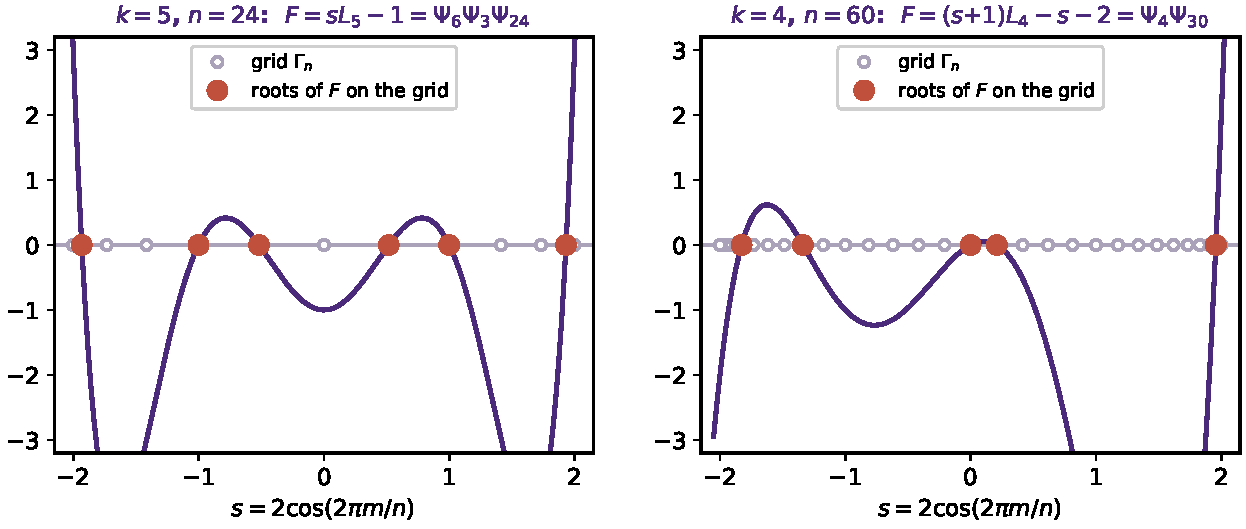
\includegraphics[width=0.92\textwidth]{figures/fig_symbol.pdf}
\caption{The 3-Parameter Symbol Curve $F(s)$ plotted against the discrete cosine grid $\Gamma_n$. Every time the curve crosses zero at a grid point $s_m \in \Gamma_n$, two conjugate Fourier blocks become singular, injecting $+2$ into the matrix nullity.}
\label{fig:symbol}
\end{figure}

\begin{thmbox}{Theorem 7.2: The 3-Parameter Symbol}
By Definition 1.10, $t_m = L_k(s_m)$ identically.
Setting inner scale $e = 1$, the singularity condition $\det M_m = 0$ is governed by a single univariate polynomial $F(s) \in \mathbb{R}[s]$:
\begin{equation}
  \det M_m = 0 \iff F(s_m) = 0,
\end{equation}
where:
\begin{equation}
  F(s) = (s + a) L_k(s) + d s + (ad - c^2) \;=\; (s + a) L_k(s) + \alpha s + \beta,
\end{equation}
with $\alpha = d$ and $\beta = ad - c^2$.
$F(s)$ is a \textbf{monic polynomial of degree $k+1$} carrying \textbf{exactly three free parameters} $(a, \alpha, \beta)$ for every $k$.
The certificate is valid (admissible) if and only if the spoke weight is real and non-zero:
\begin{equation}
  c^2 = a \alpha - \beta > 0.
\end{equation}
\end{thmbox}

\begin{defbox}{Derivation of the Linear Trick}
How do we choose $(a, \alpha, \beta)$ to make $F(s) = 0$ at desired grid points?
At any prescribed root $r$, the equation $F(r) = 0$ reads:
\begin{equation}
  (r + a) L_k(r) + \alpha r + \beta = 0 \iff a L_k(r) + \alpha r + \beta = -r L_k(r). \label{eq:root_linear}
\end{equation}
Notice that Eq.~\eqref{eq:root_linear} is \textbf{strictly linear} in the three unknowns $(a, \alpha, \beta)$.
Given any three distinct target roots $r_1, r_2, r_3$, we simply solve the $3 \times 3$ linear system:
\begin{equation}
  \begin{pmatrix}
    L_k(r_1) & r_1 & 1 \\
    L_k(r_2) & r_2 & 1 \\
    L_k(r_3) & r_3 & 1
  \end{pmatrix}
  \begin{pmatrix} a \\ \alpha \\ \beta \end{pmatrix} =
  \begin{pmatrix} -r_1 L_k(r_1) \\ -r_2 L_k(r_2) \\ -r_3 L_k(r_3) \end{pmatrix}.
\end{equation}
This solves \emph{exactly} by Gaussian elimination without any numerical search.
\end{defbox}

\begin{intubox}{Intuition: Counting Grid Roots}
Remember that $s_m = 2\cos(2\pi m / n)$:
\begin{itemize}[leftmargin=*,nosep]
  \item Because $\cos(2\pi m / n) = \cos(2\pi (n-m) / n)$, every interior grid root $s \in (-2, 2)$ corresponds to \textbf{two} distinct Fourier indices: $m$ and $n-m$.
  \item Thus, each interior root of $F(s)$ on the grid $\Gamma_n$ contributes \textbf{$+2$} to the nullity of $A$.
  \item A boundary root at $s = \pm 2$ ($m = 0$ or $m = n/2$) has $m = n-m$, contributing \textbf{$+1$}.
\end{itemize}
\end{intubox}

\begin{callbox}{Worked Numerical Example 7.1: The Exact $3 \times 3$ Linear Solve for Prescribed Roots}
Let us solve the $3 \times 3$ linear system for $k=2$ with concrete target roots.
The degree-2 Chebyshev basis polynomial is $L_2(s) = s^2 - 2$.
Suppose we prescribe the three target roots:
\begin{equation}
  r_1 = -1, \qquad r_2 = \frac{1+\sqrt{5}}{2} \approx 1.61803, \qquad r_3 = \frac{1-\sqrt{5}}{2} \approx -0.61803.
\end{equation}
Notice that $r_2$ and $r_3$ are the golden ratio and its conjugate, satisfying $r^2 - r - 1 = 0 \iff r^2 - 2 = r - 1$.
Evaluating $L_2(r)$ at each root:
\begin{itemize}[leftmargin=*,nosep]
  \item At $r_1 = -1$: $L_2(-1) = (-1)^2 - 2 = -1$.
  \item At $r_2$: $L_2(r_2) = r_2 - 1 = \frac{\sqrt{5}-1}{2}$.
  \item At $r_3$: $L_2(r_3) = r_3 - 1 = \frac{-\sqrt{5}-1}{2}$.
\end{itemize}
The right-hand side vector has entries $-r L_2(r)$:
\begin{itemize}[leftmargin=*,nosep]
  \item For $r_1$: $-(-1)(-1) = -1$.
  \item For $r_2$: $-r_2(r_2 - 1) = -(r_2^2 - r_2) = -(1) = -1$.
  \item For $r_3$: $-r_3(r_3 - 1) = -(r_3^2 - r_3) = -(1) = -1$.
\end{itemize}
The $3 \times 3$ linear equation system reads:
\begin{equation}
  \begin{pmatrix}
    -1 & -1 & 1 \\
    r_2 - 1 & r_2 & 1 \\
    r_3 - 1 & r_3 & 1
  \end{pmatrix}
  \begin{pmatrix} a \\ \alpha \\ \beta \end{pmatrix} =
  \begin{pmatrix} -1 \\ -1 \\ -1 \end{pmatrix}.
\end{equation}
Notice that every row on the right-hand side is $-1$.
Testing the candidate vector $[a, \alpha, \beta]^T = [0, 0, -1]^T$:
\begin{align}
  \text{Row 1: } & 0(-1) + 0(-1) + 1(-1) = -1, \quad \checkmark \\
  \text{Row 2: } & 0(r_2 - 1) + 0(r_2) + 1(-1) = -1, \quad \checkmark \\
  \text{Row 3: } & 0(r_3 - 1) + 0(r_3) + 1(-1) = -1. \quad \checkmark
\end{align}
The solution is uniquely and exactly:
\begin{equation}
  a = 0, \qquad \alpha = 0, \qquad \beta = -1.
\end{equation}
Now check the spoke weight admissibility:
\begin{equation}
  c^2 = a\alpha - \beta = (0)(0) - (-1) = \mathbf{1} > 0 \implies c = 1.
\end{equation}
Because $c^2 = 1 > 0$, the certificate is valid, real, and strictly non-zero.
The resulting matrix $A$ has outer diagonal $a=0$, inner diagonal $d=\alpha=0$, spoke weight $c=1$, and inner chord weight $e=1$.
This is precisely the unweighted adjacency matrix $A = \operatorname{Adj}(P(n,2))$.
\end{callbox}

\newpage

%% =========================================================================
%% SECTION 8: THE CYCLOTOMIC BREAKTHROUGH
%% =========================================================================
\section{Cyclotomic Certificates: Galois Orbits and Exact Integer Matrices}

\subsection{A Claim of Ours, Corrected: Period-One Is Not Capped at 6}

\begin{callbox}{A claim of ours, corrected}
An earlier draft of this project asserted that period-one equivariant certificates could never achieve nullity greater than $6$ for any $k \ge 2$.
\begin{itemize}[leftmargin=*,nosep]
  \item \textbf{The flawed reasoning}: ``The linear system in Eq.~\eqref{eq:root_linear} has only 3 unknowns. Therefore, you can only prescribe 3 roots. Three roots contribute $3 \times 2 = 6$ to nullity. Therefore, period-1 is capped at 6.''
  \item \textbf{Why this reasoning is wrong}: While you can only \emph{prescribe} 3 roots, prescribing those 3 roots automatically determines the remaining $(k+1) - 3 = k - 2$ roots.
  \item If the polynomial $F(s)$ has \textbf{rational coefficients}, its roots must form complete \textbf{Galois orbits}.
  \item By Theorem 1.3, if one root of a minimal polynomial $\Psi_d(s)$ is on the grid $\Gamma_n$, \emph{its entire Galois orbit lands on the grid automatically}.
  \item Arithmetic pulls all $k+1$ roots onto the grid at once, unlocking the full ceiling $2k+2$.
\end{itemize}
\end{callbox}

\subsection{Theorem: Exact Cyclotomic Matrix Certificates}

\begin{thmbox}{Theorem 8.1: Exact Cyclotomic Matrix Certificates}
Let $D = \{d_1, d_2, \dots, d_p\}$ be a collection of distinct positive integers such that:
\begin{equation}
  \sum_{d \in D} \deg(\Psi_d) = k + 1.
\end{equation}
Define the candidate symbol $F(s) = \prod_{d \in D} \Psi_d(s) \in \mathbb{Z}[s]$.
Let $G(s) = F(s) - s L_k(s)$, and let $a \in \mathbb{Z}$ be the coefficient of $s^k$ in $G(s)$.
If the polynomial $G(s) - a L_k(s)$ has degree at most 1:
\begin{equation}
  G(s) - a L_k(s) = \alpha s + \beta, \qquad (\alpha, \beta \in \mathbb{Z}),
\end{equation}
and if $c^2 = a\alpha - \beta > 0$, then:
For every $n$ divisible by $\operatorname{lcm}(\mathcal D)$ with $n > 2k$, the explicit integer matrix
\begin{equation}
  A = \begin{pmatrix} a I + P + P^{-1} & c I \\ c I & \alpha I + P^k + P^{-k} \end{pmatrix} \in S(P(n,k))
\end{equation}
has nullity exactly:
\begin{equation}
  \operatorname{null}(A) = 2 \sum_{d \in D, \, d \ge 3} \deg(\Psi_d) + \# \{ d \in D \mid d \le 2 \}.
\end{equation}
If all $d \in D$ satisfy $d \ge 3$, the nullity equals the theoretical ceiling:
\begin{equation}
  \operatorname{null}(A) = 2(k + 1) = 2k + 2.
\end{equation}
Consequently, for all such $n$:
\begin{equation}
  Z(P(n, k)) = M(P(n, k)) = 2k + 2.
\end{equation}
\end{thmbox}

\begin{table}[htbp]
\centering
\begin{tabular}{clllrrrr}
\toprule
$k$ & $\mathcal D$ & $\operatorname{lcm}(\mathcal D)$ & Symbol $F(s)$ & $a$ & $d$ & $c^2$ & Exact Nullity \\
\midrule
2 & $\{3, 10\}$ & 30 & $s L_2(s) - 1$ & 0 & 0 & 1 & $6 = 2k+2$ \\
2 & $\{14\}$ & 14 & $\Psi_{14}(s)$ & $-1$ & 0 & 1 & $6 = 2k+2$ \\
3 & $\{1, 4, 5\}$ & 20 & $\Psi_1 \Psi_4 \Psi_5$ & $-1$ & $-1$ & 1 & 7 \\
\textbf{4} & $\mathbf{\{4, 30\}}$ & \textbf{60} & $\mathbf{(s+1)L_4(s) - s - 2}$ & \textbf{1} & $\mathbf{-1}$ & \textbf{1} & $\mathbf{10 = 2k+2}$ \\
\textbf{4} & $\mathbf{\{5, 14\}}$ & \textbf{70} & $\mathbf{\Psi_5 \Psi_{14}}$ & \textbf{0} & \textbf{1} & \textbf{1} & $\mathbf{10 = 2k+2}$ \\
\textbf{4} & $\mathbf{\{5, 18\}}$ & \textbf{90} & $\mathbf{\Psi_5 \Psi_{18}}$ & \textbf{1} & \textbf{0} & \textbf{1} & $\mathbf{10 = 2k+2}$ \\
\textbf{5} & $\mathbf{\{3, 6, 24\}}$ & \textbf{24} & $\mathbf{s L_5(s) - 1}$ & \textbf{0} & \textbf{0} & \textbf{1} & $\mathbf{12 = 2k+2}$ \\
\bottomrule
\end{tabular}
\caption{Exact Integer Cyclotomic Matrix Certificates. For $k=4$ and $k=5$ these are, as far as we know, the first exact values at any $k \ge 4$.}
\label{tab:cyclotomic}
\end{table}

\subsection{The Complete Adjacency Matrix Classification Theorem}

Notice from Table~\ref{tab:cyclotomic} that for $k=2$ and $k=5$, the parameters are $a=0, d=0, c=1$.
This means the certificate is \textbf{the unweighted adjacency matrix itself}: $A = \operatorname{Adj}(P(n,k))$.
When is the plain adjacency matrix of $P(n,k)$ singular, and what is its exact nullity?

\begin{thmbox}{Theorem 8.2: Classification of Adjacency Matrix Nullity}
Define the integer polynomial:
\begin{equation}
  P_k(z) = z^{2k+2} + z^{2k} - z^{k+1} + z^2 + 1 \in \mathbb{Z}[z].
\end{equation}
For any $n > 2k$, the nullity of the adjacency matrix of $P(n,k)$ is given by the exact closed formula:
\begin{equation}
  \operatorname{null}(\operatorname{Adj} P(n,k)) = \sum_{\substack{d \,:\, \Phi_d(z) \mid P_k(z) \\ d \mid n}} \varphi(d),
\end{equation}
where $\Phi_d(z)$ is the $d$-th cyclotomic polynomial.
\end{thmbox}

\begin{defbox}{Proof via Conway--Jones Theory}
For the adjacency matrix, $a=0, d=0, c=1$. The Fourier block determinant is:
\begin{equation}
  \det M_m = s_m t_m - 1 = \left(2\cos\frac{2\pi m}{n}\right)\left(2\cos\frac{2\pi km}{n}\right) - 1 = 0.
\end{equation}
Using the product-to-sum trigonometric identity $2\cos A \cos B = \cos(A+B) + \cos(A-B)$:
\begin{equation}
  2\cos\frac{2\pi(k+1)m}{n} + 2\cos\frac{2\pi(k-1)m}{n} = 1.
\end{equation}
Let $z = e^{2\pi i m / n}$. Express cosines as complex exponentials $2\cos\theta = z + z^{-1}$:
\begin{equation}
  (z^{k+1} + z^{-(k+1)}) + (z^{k-1} + z^{-(k-1)}) = 1.
\end{equation}
Multiply through by $z^{k+1}$ to clear denominators:
\begin{equation}
  (z^{2k+2} + 1) + (z^{2k} + z^2) - z^{k+1} = 0 \iff P_k(z) = 0.
\end{equation}
Therefore, Fourier block $m$ is singular if and only if $z = e^{2\pi i m / n}$ is a root of $P_k(z)$.
Because $z$ is an $n$-th root of unity, $z$ must be a common root of $P_k(z)$ and $z^n - 1$.
The roots of unity dividing $P_k(z)$ are precisely the roots of its cyclotomic factors $\Phi_d(z)$.
A primitive $d$-th root of unity belongs to $\mathbb{Z}_n$ if and only if $d$ divides $n$.
Each cyclotomic factor $\Phi_d(z)$ contributes exactly its $\deg(\Phi_d) = \varphi(d)$ roots. \qedhere
\end{defbox}

\begin{table}[htbp]
\centering
\begin{tabular}{crlrl}
\toprule
$k$ & Ceiling $2k+2$ & Cyclotomic Factors of $P_k(z)$ & $\operatorname{lcm}$ & Nullity when $\operatorname{lcm} \mid n$ \\
\midrule
2 & 6 & $\Phi_3, \, \Phi_{10}$ & 30 & $6 = 2k+2$ (Attains Ceiling.) \\
\textbf{3} & \textbf{8} & \textbf{None} & --- & \textbf{0 (Never singular for any $n$.)} \\
4 & 10 & $\Phi_3$ & 3 & 2 \\
5 & 12 & $\Phi_3, \, \Phi_6, \, \Phi_{24}$ & 24 & $12 = 2k+2$ (Attains Ceiling.) \\
\textbf{6} & \textbf{14} & \textbf{None} & --- & \textbf{0 (Never singular for any $n$.)} \\
7 & 16 & $\Phi_3, \, \Phi_6$ & 6 & 4 \\
8 & 18 & $\Phi_3, \, \Phi_{10}$ & 30 & 6 \\
\textbf{9} & \textbf{20} & \textbf{None} & --- & \textbf{0 (Never singular for any $n$.)} \\
\bottomrule
\end{tabular}
\caption{Complete cyclotomic factorization of $P_k(z)$. Note the Conway--Jones phenomenon: the adjacency matrix of $P(n,k)$ is \textbf{strictly non-singular for all $k \equiv 0 \pmod 3$}.}
\label{tab:adj_class}
\end{table}

\begin{callbox}{Worked Numerical Example 8.1: Adjacency Nullity for $P(18, 4)$ vs $P(18, 3)$}
Let us apply the Conway--Jones classification formula (Theorem 8.2) to evaluate the exact nullity of the adjacency matrix for $n=18$ at $k=4$ and $k=3$:
\begin{itemize}[leftmargin=*,nosep]
  \item \textbf{Case $k=4$ on $P(18, 4)$}:
  The polynomial is $P_4(z) = z^{10} + z^8 - z^5 + z^2 + 1$.
  Factoring over $\mathbb{Z}[z]$:
  \begin{equation}
    P_4(z) = (z^2 + z + 1) \cdot (z^8 - z^7 + z^5 - 2z^4 + z^3 - z + 1) = \Phi_3(z) \cdot Q(z),
  \end{equation}
  where $Q(z)$ has no roots on the unit circle.
  The only cyclotomic factor is $\Phi_3(z)$, which corresponds to $d=3$.
  Since $d = 3$ divides $n = 18$ ($18 / 3 = 6 \in \mathbb{Z}$), this factor is active.
  Applying the formula:
  \begin{equation}
    \operatorname{null}(\operatorname{Adj} P(18, 4)) = \sum_{d \mid 18, \, \Phi_d \mid P_4} \varphi(d) = \varphi(3) = \mathbf{2}.
  \end{equation}
  The two singular Fourier modes correspond to $m = 6$ and $m = 12$.
  At $m=6$, $z = e^{2\pi i (6)/18} = e^{2\pi i / 3}$, which satisfies $\Phi_3(z) = 0$.

  \item \textbf{Case $k=3$ on $P(18, 3)$}:
  The polynomial is $P_3(z) = z^8 + z^6 - z^4 + z^2 + 1$.
  Factoring reveals that $P_3(z)$ is \textbf{strictly irreducible over $\mathbb{Z}[z]$} and is not cyclotomic.
  It has \textbf{zero cyclotomic factors}:
  \begin{equation}
    \{ d \mid \Phi_d(z) \text{ divides } P_3(z) \} = \emptyset.
  \end{equation}
  Therefore, the formula gives:
  \begin{equation}
    \operatorname{null}(\operatorname{Adj} P(18, 3)) = \mathbf{0}.
  \end{equation}
  The unweighted adjacency matrix of $P(18, 3)$ is completely invertible.
  In fact, for any $n$, the adjacency matrix of $P(n,3)$ is never singular.
\end{itemize}
\end{callbox}

\newpage

%% =========================================================================
%% SECTION 9: GENERAL CYCLIC COVERS & FLOQUET THEORY
%% =========================================================================
%% =========================================================================
%% SECTION 9: ALL LARGE n -- TILES, KRAWCZYK, EXACT ARITHMETIC
%% =========================================================================
\section{All Large $n$ at Once: Identity Tiles and Certified Arithmetic}

Sections 7 and 8 produce certificates one $n$ at a time, and only for $n$ in a divisibility class. This section explains the construction that settles \emph{every} $n$ past a threshold, and what it means to say that the result is certified.

\subsection{Why Period-One Certificates Are Confined to Divisibility Classes}

\begin{thmbox}{Theorem 9.1: Period-one certificates live on divisibility classes}
Let $A$ be a period-one matrix with symbol $F$ (Theorem 7.2) and suppose $\operatorname{null}A=2k+2$ for some $n>2k$. Then every root of $F$ is of the form $2\cos(2\pi j/d)$ with $\gcd(j,d)=1$ and $d\ge3$, and the set of $n$ at which \emph{this same matrix} attains the ceiling is exactly
\begin{equation}
  \{\,n:\ \operatorname{lcm}(\mathcal D)\mid n\,\},
\end{equation}
where $\mathcal D$ is the set of those $d$. This set has density at most $1/3$ and contains at most one prime.
\end{thmbox}

\begin{intubox}{Intuition: a fixed polynomial can only hit a fixed grid}
The symbol $F$ is a polynomial that does not change with $n$. Its roots are fixed real numbers. The grid $\Gamma_n=\{2\cos(2\pi m/n)\}$ changes with $n$. A root $2\cos(2\pi j/d)$ lies on the grid $\Gamma_n$ exactly when $d$ divides $n$. So one period-one matrix can serve all multiples of $\operatorname{lcm}(\mathcal D)$ --- and no other $n$. Primes are the extreme case: a prime $p$ is on the list only if $\operatorname{lcm}(\mathcal D)=p$, which can happen for at most one $p$.
\end{intubox}

\begin{callbox}{Worked Numerical Example 9.1: Which $n$ does the $k=4$ certificate reach?}
Table~\ref{tab:cyclotomic} gives at $k=4$ the symbol $F=\Psi_4\Psi_{30}$, so $\mathcal D=\{4,30\}$ and $\operatorname{lcm}(\mathcal D)=60$. The matrix with $a=1$, $d=-1$, $c=1$ has nullity $10$ exactly at $n\in\{60,120,180,\dots\}$: at $n=60$ the grid $\Gamma_{60}$ contains $2\cos(2\pi/4)=0$ and all four roots of $\Psi_{30}$; at $n=61$ (a prime) it contains neither. So three certificates ($\operatorname{lcm}=60,70,90$) together cover only $n\in60\mathbb Z\cup70\mathbb Z\cup90\mathbb Z$, a set of density $1/60+1/70+1/90-\dots\approx0.040$. Nothing period-one reaches $n=61$, $n=67$, or any other prime.
\end{callbox}

\subsection{Exactly Which $n$ a Rational Symbol Can Reach}

\begin{thmbox}{Theorem 9.2: Classification of rational-symbol certificates}
Fix $k\ge2$. A symmetric rotation-invariant matrix on $P(n,k)$ whose symbol has rational coefficients and nullity $2k+2$ exists if and only if $n>2k$ and $n$ is divisible by one of
\[
  7,9,15,20\ (k=2);\quad 10,24,42\ (k=3);\quad 60,70,90\ (k=4);\quad 24,126\ (k=5);\quad \text{none}\ (k=6);\quad 120\ (k=7).
\]
\end{thmbox}

\begin{intubox}{Why this is a finite problem}
Rational coefficients force the root set of the symbol to be closed under the Galois group: if $2\cos(2\pi/d)$ is a root, so is every $2\cos(2\pi j/d)$ with $\gcd(j,d)=1$. So the roots are a union of whole orbits $O_d$, of sizes $\varphi(d)/2$, adding up to $k+1$. That bounds $d$ and leaves finitely many candidate sets. Each candidate is tested by two exact computations: the product of the minimal polynomials $\Psi_d$ must agree with $(s+a)(t_k(s)+d')-c_0$ in all its middle coefficients (the ``three free parameters'' of Theorem 7.2, now as $k-2$ forced equations), and $c_0\ne0$ so that the spoke weight is nonzero.
\end{intubox}

\begin{callbox}{Worked Example 9.2: $k=3$, the set $\{3,6,8\}$}
Orbits: $O_3=\{-1\}$, $O_6=\{1\}$, $O_8=\{\pm\sqrt2\}$; four roots, as $k+1$ requires. The monic product is $(s+1)(s-1)(s^2-2)=s^4-3s^2+2$. With $t_3(s)=s^3-3s$ and $a=[s^3]=0$, the difference $s^4-3s^2+2-s\,t_3(s)=2$ has degree $0$, so $d'=0$ and $c_0=a d'-2=-2\ne0$: realisable, with $e=-1$ and $c=\sqrt2$. The roots lie on the grid of $P(n,3)$ exactly when $\operatorname{lcm}(3,6,8)=24$ divides $n$, and there the matrix has nullity $8$. Compare $\{3,9\}$: product $(s+1)(s^3-3s+1)=s^4+s^3-3s^2-2s+1$ and $a=1$; since $(s+1)t_3(s)=s^4+s^3-3s^2-3s$, the difference is $s+1$, giving $d'=1$, constant $1$, and $c_0=a d'-1=0$. Not realisable: the spoke weight would vanish.
\end{callbox}

\subsection{Tiles: Pieces Whose Monodromy Is the Identity}

Recall (Section 6) that for \emph{any} matrix on the $P(n,k)$ pattern the kernel is governed by a recurrence of order $2k+2$, with step matrices $T_i$ and monodromy $T=T_{n-1}\cdots T_0$, and that $\operatorname{null}A=2k+2$ exactly when $T=I$. The condition $T=I$ is \emph{multiplicative along the cycle}. That suggests building the weight sequence from pieces each contributing the identity.

\begin{defbox}{Definition 9.1: Docking pattern, tile, interior}
Fix $k$. A \textbf{docking pattern} is a fixed choice of the five weights $(b,c,e,a,d)$ at $k+1$ consecutive positions. A \textbf{tile} of length $\ell\ge2(k+1)$ is a weight sequence of length $\ell$ whose first $k+1$ and last $k+1$ positions carry the docking pattern. Its \textbf{interior} is the remaining $\ell-2(k+1)$ positions, which are free. The \textbf{tile product} is $T_{\text{tile}}=T_{s+\ell-1}\cdots T_{s}$, the product of the step matrices over the tile's positions.
\end{defbox}

\begin{figure}[htbp]
\centering
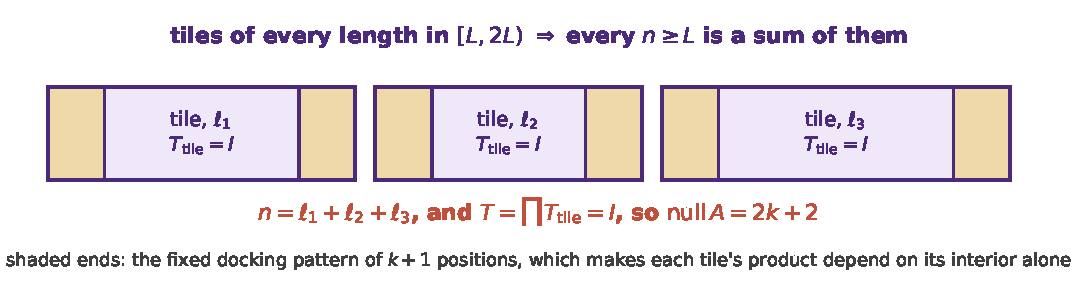
\includegraphics[width=0.85\textwidth]{figures/fig_tiling.pdf}
\caption{Tiles of every length in $[L,2L)$ cover every $n\ge L$: write $n$ as a sum of tile lengths, concatenate the tiles, and the monodromy is the product of the tile products. Shared docking patterns at the ends make the products independent of their neighbours.}
\label{fig:tiling}
\end{figure}

\begin{thmbox}{Lemma 9.2: Tile independence}
If the weight sequence on $\mathbb Z_n$ is a concatenation of tiles sharing one docking pattern, then each tile's product depends only on that tile's interior weights, and the monodromy $T$ is the product of the tile products.
\end{thmbox}

\begin{defbox}{Why the lemma is true (the window argument)}
By Theorem 6.1, the step matrix $T_i$ is built from the coefficients $\gamma_{i,p}$, which involve the weights at indices in the window $[i-k-1,\,i+k]$ only. If the tile occupies positions $[s,s+\ell)$ and $i$ is inside it, the window is contained in $[s-k-1,\,s+\ell+k-1]$. The part of that window below $s$ lies in the \emph{previous} tile's last $k+1$ positions; the part at or above $s+\ell$ lies in the \emph{next} tile's first $k+1$ positions. Both carry the docking pattern, which is the same for every tile. So every weight $T_i$ can see is either docking (fixed and identical everywhere) or in this tile's own interior. The second claim is just associativity of the product regrouped tile by tile.
\end{defbox}

\begin{thmbox}{Theorem 9.3: Tiling}
Fix $k$ and $L\ge2(k+1)$. Suppose that for every length $\ell$ with $L\le\ell<2L$ there is a tile of length $\ell$ with all required weights nonzero and $T_{\text{tile}}=I$. Then
\begin{equation}
  Z(P(n,k))=M(P(n,k))=2k+2\qquad\text{for every }n\ge L,
\end{equation}
with no congruence condition on $n$.
\end{thmbox}

\begin{defbox}{Proof}
Every $n\ge L$ is a sum of integers from $[L,2L)$: if $n<2L$ take $n$ itself; if $n\ge2L$ take one term $L$ and recurse on $n-L\ge L$. Concatenate the tiles of those lengths. By Lemma 9.2 the monodromy is the product of the tile products, each $I$, so $T=I$; all weights are nonzero, so the matrix carries the pattern of $P(n,k)$; by Corollary 6.3, $\operatorname{null}A=2k+2$. Then $2k+2=\operatorname{null}A\le M\le Z\le2k+2$, the last by the rotation bootstrap (Theorem 4.1). \qedhere
\end{defbox}

\begin{callbox}{Worked Numerical Example 9.2: Writing $n$ as a sum of tile lengths at $k=3$}
At $k=3$ the certified tile lengths are every $\ell$ in $[21,44)$, so $L=21$. Decompose:
\begin{itemize}[leftmargin=*,nosep]
  \item $n=37$: already in $[21,42)$, one tile of length $37$.
  \item $n=45$: $45\ge42$, so take $21$ and recurse on $24\in[21,42)$: $45=21+24$.
  \item $n=100$: $100\to21+79\to21+21+58\to21+21+21+37$, and $37\in[21,42)$. So $100=21+21+21+37$, four tiles.
  \item $n=101$ (a prime): $101=21+21+21+38$. The construction does not care that $101$ is prime --- this is exactly what Theorem 9.1 says period-one matrices cannot do.
\end{itemize}
Why a full interval $[L,2L)$ is needed: with only two lengths $a,b$ one gets just the sums $ia+jb$, which miss every $n<(a-1)(b-1)$ --- for $a=21,b=22$ that is every $n<420$.
\end{callbox}

\subsection{Where the Tiles Come From: Counting Equations}

\begin{callbox}{Worked Numerical Example 9.3: The parameter count at $k=3$}
A tile of length $\ell$ has $\ell-2(k+1)=\ell-8$ interior positions, each carrying five free weights: $5(\ell-8)$ unknowns. The condition $T_{\text{tile}}=I$ is an equation between $(2k+2)\times(2k+2)=8\times8$ matrices: $64$ equations. Solvability on parameter count needs $5(\ell-8)\ge64$, i.e.\ $\ell\ge20.8$, so $\ell\ge21$. In practice:
\begin{itemize}[leftmargin=*,nosep]
  \item $\ell=19$: $55$ unknowns against $64$ equations --- the Newton residual stalls near $0.4$.
  \item $\ell=20$: $60$ unknowns --- stalls likewise.
  \item $\ell=21$: $65$ unknowns, the first length with more unknowns than equations --- a solution with residual $10^{-14}$ exists, found on the $25$th random restart after four restarts had stalled at $0.056$.
\end{itemize}
The last point is recorded in the paper as a caution: a failed search measures the effort spent, not impossibility.
\end{callbox}

The solve itself is a damped Newton iteration on the $64$ (or $(2k+2)^2$) equations $T_{\text{tile}}(w)-I=0$ from random starts. A numerical solution with residual $10^{-14}$ is strong evidence, but it is not a proof that an \emph{exact} tile exists. For that the project uses interval arithmetic.

\subsection{Krawczyk's Existence Test}

\begin{defbox}{Definition 9.2: Interval boxes and the Krawczyk operator}
Let $f:\mathbb R^m\to\mathbb R^m$ be continuously differentiable, let $X\subset\mathbb R^m$ be a box (a product of intervals) with centre $x_0$, let $J(X)$ denote an interval matrix containing the Jacobian $f'(x)$ for every $x\in X$, and let $Y$ be \emph{any} fixed $m\times m$ matrix (in practice an approximate inverse of $f'(x_0)$). The \textbf{Krawczyk operator} is
\begin{equation}
  K(X)\;=\;x_0-Y\,f(x_0)\;+\;\bigl(I-Y\,J(X)\bigr)\,(X-x_0),
\end{equation}
evaluated in interval arithmetic, so that $K(X)$ is again a box.
\end{defbox}

\begin{thmbox}{Theorem 9.4: Krawczyk (Moore--Kearfott--Cloud)}
If $K(X)\subseteq\operatorname{int}X$ and $Y$ is nonsingular, then $f$ has exactly one zero in $X$. A sufficient, checkable form: with $\alpha=\|I-YJ(X)\|_\infty$ and $\delta$ the radius of $X$, if
\begin{equation}
  \alpha<1\qquad\text{and}\qquad \|Y f(x_0)\|_\infty+\alpha\,\delta\;\le\;\delta,
\end{equation}
then a true zero of $f$ exists in $X$.
\end{thmbox}

\begin{intubox}{Intuition: a contraction that cannot escape the box}
$K$ is Newton's step written so that every possible Jacobian over the whole box is accounted for at once. If applying $K$ to the box lands strictly inside the box, the Newton map is a contraction on $X$ and must have a fixed point there --- a genuine zero of $f$, not a floating-point approximation of one. You never find the zero exactly; you prove it is inside a box of radius $\delta$.
\end{intubox}

\begin{callbox}{Worked Numerical Example 9.4: Certifying $\sqrt2$ in one dimension}
Let $f(x)=x^2-2$, $X=[1.41,\,1.42]$, $x_0=1.415$, $\delta=0.005$.
\begin{itemize}[leftmargin=*,nosep]
  \item $f(x_0)=1.415^2-2=0.002225$.
  \item $f'(x)=2x$, so over $X$ the Jacobian interval is $J(X)=[2.82,\,2.84]$.
  \item Take $Y=1/f'(x_0)=1/2.83=0.35336$.
  \item $I-YJ(X)=1-0.35336\cdot[2.82,2.84]=[-0.00353,\,0.00353]$, so $\alpha=0.00353<1$.
  \item $K(X)=x_0-Yf(x_0)+(I-YJ(X))(X-x_0)=1.415-0.000786+[-0.00353,0.00353]\cdot[-0.005,0.005]$ \\ $=[1.414196,\,1.414231]$.
\end{itemize}
Since $[1.414196,1.414231]\subset(1.41,1.42)$, a zero of $f$ exists in $X$; indeed $\sqrt2=1.414214\ldots$ The check form: $\|Yf(x_0)\|+\alpha\delta=0.000786+0.0000177=0.000804\le0.005$.
\end{callbox}

\subsection{How the Project Applies It, and Why ``Exact'' Is Exact}

The unknowns are the tile's interior weights $w$ together with a candidate kernel basis $X$ of size $2k+2$; the equation is the bilinear system $f(w,X)=A(w)K(X)=0$, written in a ``graph form'' that fixes the gauge so that the square subsystem used is \emph{equivalent} to $AK=0$ rather than a maximal-rank selection from it (the paper's Section on exact certification explains that distinction). Krawczyk passing proves that a true real solution exists in a box of radius $\delta\approx10^{-13}$ around the numerical one --- hence a real matrix with the $P(n,k)$ pattern and nullity $\ge2k+2$, hence exactly $2k+2$ by the ceiling.

\begin{callbox}{Three observations that make the test exact (Section on exact arithmetic of the paper)}
\begin{enumerate}[leftmargin=*,nosep]
  \item The box centre is a float64 vector; every float64 is a dyadic rational. Snap it to $2^{-60}\mathbb Z$; it is now \emph{known exactly}.
  \item $f(w,X)=A(w)K(X)$ is bilinear with integer coefficients, so $J(z_0)$ and $f(z_0)$ are exact rationals with denominators $2^{60}$ and $2^{120}$.
  \item $Y$ is arbitrary in Theorem 9.4; take the float64 inverse and read it as an exact dyadic rational, losing nothing.
\end{enumerate}
Then $\|Y\|_\infty$, $\alpha$ and $\|Yf(z_0)\|_\infty$ are exact rationals and the two comparisons are integer comparisons. The one cost is speed: $YJ(z_0)$ is a product of integer matrices of size up to $1175$. It is computed by splitting each integer into base-$2^{20}$ digits, multiplying digit matrices in float64 (where products stay below $2^{53}$ and are therefore exact), and recombining in integer arithmetic.
\end{callbox}

\begin{callbox}{Worked Numerical Example 9.5: The two certifications the thresholds rest on}
\begin{center}
\begin{tabular}{crrrr}
\toprule
tile & size of $J$ & $\|Y\|_\infty$ & $\alpha$ & verdict \\
\midrule
$k=3$, $\ell=21$ & $308\times308$ & $1.5743\times10^{3}$ & $2.139912\times10^{-10}$ & passes at $\delta=10^{-13}$ \\
$k=4$, $\ell=29$ & $535\times535$ & $1.4416\times10^{3}$ & $1.822215\times10^{-10}$ & passes at $\delta=10^{-13}$ \\
\bottomrule
\end{tabular}
\end{center}
$\alpha$ is ten orders of magnitude below the threshold $1$. The float64 and exact values agree to three figures --- expected, and the reason the original conclusion was never in doubt. The point is that the exact numbers are \emph{bounds}, the float64 ones were \emph{estimates}.
\end{callbox}

\subsection{What the Tiles Settle}

\begin{thmbox}{Theorem 9.5: All large $n$, for $k=3$, $4$ and $5$}
With tiles certified at every length in $[21,44)$ for $k=3$, in $[29,62)$ for $k=4$, and at the lengths $\{54,\dots,72,74,75\}$ for $k=5$ (which do not fill an interval $[L,2L)$ but generate every $n\ge\SettleFive$ as a sum):
\begin{align}
  Z(P(n,3))&=M(P(n,3))=8 &&\text{for every } n\ge17,\\
  Z(P(n,4))&=M(P(n,4))=10 &&\text{for every } n\ge\SettleFour,\\
  Z(P(n,5))&=M(P(n,5))=12 &&\text{for every } n\ge\SettleFive.
\end{align}
The $k=3$ range starts at $17$ rather than $21$ because $n=17,18,19,20$ carry individual Krawczyk-certified matrices. All $\NtileAll$ tiles and all $\NcertGN$ per-$n$ matrices are certified in exact rational arithmetic with $\alpha\le\MaxAlpha$.
\end{thmbox}

\begin{thmbox}{Theorem 9.6: Complete determination for $k=2,3,4$}
Combining Theorem 9.5 with exhaustive search for every smaller $n$, $Z(P(n,k))$ is known for \emph{every} admissible $n$ at $k=2$, $k=3$ and $k=4$. In particular
\begin{equation}
  Z(P(n,3))=8\quad\text{for every }n\ge13,\qquad\text{and }13\text{ is optimal.}
\end{equation}
\end{thmbox}

\begin{callbox}{Worked Numerical Example 9.6: The $k=3$ row, and what was wrong in the literature}
\begin{center}
\begin{tabular}{c|cccccccccccccc}
$n$ & 7 & 8 & 9 & 10 & 11 & 12 & 13 & 14 & 15 & 16 & 17 & 18 & 19 & 20 \\
\hline
$Z(P(n,3))$ & 6 & 6 & 6 & 8 & 7 & 7 & 8 & 8 & 8 & 8 & 8 & 8 & 8 & 8
\end{tabular}
\end{center}
The row is not monotone: it reaches $8$ at $n=10$, drops to $7$ at $n=11,12$, and settles at $13$. Rashidi, Shajareh Poursalavati and Tavakkoli (2020) had claimed $Z(P(n,3))=8$ for all $n\ge12$; Krishnan (arXiv:2607.19412, July 2026) found $Z(P(12,3))=7$ by exhibiting a $7$-vertex forcing set and confirming by exhaustive search that no $6$-vertex set forces, computed the row above, and stated as Conjecture~5 that $Z(P(n,3))=8$ for every $n\ge13$, writing that ``the missing ingredient is a lower-bound proof valid for all large $n$''. The lower bound is Theorem 9.5 (a matrix of nullity $8$ for every $n\ge17$) together with exhaustive search at $n=13,14,15,16$. \textbf{Division of credit}: the correction to the published value is Krishnan's; the proof of his conjecture, and the first exact values at $k=4$, are this project's.
\end{callbox}

\begin{intubox}{What the matrix statement adds over the forcing statement}
$Z=8$ is a combinatorial fact. $M=8$ says more: there is a real symmetric matrix with that graph's wiring whose zero eigenvalue has multiplicity $8$, the largest the wiring allows. The two agree on $P(n,k)$ at $k=2,3,4$; Section 10 shows they need not agree on other cyclic covers.
\end{intubox}

\newpage
%% =========================================================================
%% SECTION 10: CYCLIC COVERS -- REDUCTION, REFUTATIONS, THE RIGHT HYPOTHESIS
%% =========================================================================
\section{The General Setting: Cyclic Covers, and Two Refutations}

Nothing in Sections 6--9 used the particular shape of $P(n,k)$ beyond the rotation. This section states the general setting, says exactly how far the ceiling extends, and records two conjectures of this project that turned out to be false --- the second of which had been presented as its strongest result.

\subsection{Voltage Graphs and Derived Graphs}

\begin{defbox}{Definition 10.1: Voltage assignment and cyclic cover}
Let $B$ be a finite graph (loops and parallel edges allowed) and give each edge $x\!-\!y$ an orientation and a \textbf{voltage} $v\in\mathbb Z_n$ (no loop may carry voltage $0$). The \textbf{derived graph} or \textbf{cyclic cover} $B^n$ has vertex set $V(B)\times\mathbb Z_n$, and for each edge $x\!-\!y$ of voltage $v$ and each $i\in\mathbb Z_n$ an edge
\begin{equation}
  (x,i)\ \sim\ (y,\,i+v).
\end{equation}
The set $\{(x,i):i\in\mathbb Z_n\}$ is the \textbf{fibre} over $x$. The rotation $(x,i)\mapsto(x,i+1)$ is an automorphism of $B^n$.
\end{defbox}

\begin{figure}[htbp]
\centering
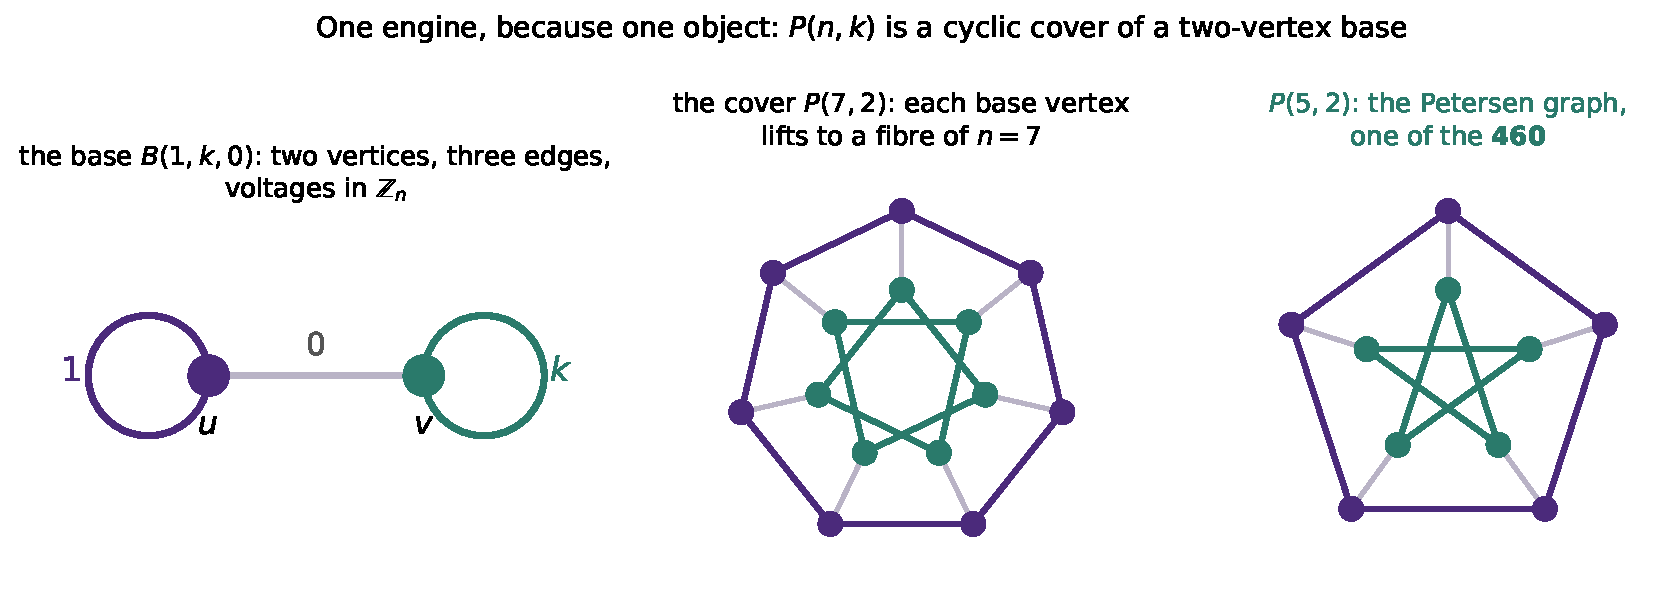
\includegraphics[width=0.95\textwidth]{figures/fig_cover.pdf}
\caption{One engine, one object. Left: the two-vertex base $B(1,k,0)$ --- a loop of voltage $1$ at $u$, a loop of voltage $k$ at $v$, an edge $u\!-\!v$ of voltage $0$. Middle: its cover with $n=7$, $k=2$, each base vertex lifted to a fibre of $7$. Right: $n=5$, $k=2$ is the Petersen graph.}
\label{fig:cover}
\end{figure}

\begin{callbox}{Worked Numerical Example 10.1: Two covers written out}
\textbf{(a) $P(n,k)$.} Base: vertices $u,v$; loop at $u$ of voltage $1$; loop at $v$ of voltage $k$; edge $u\!-\!v$ of voltage $0$. The cover has $(u,i)\sim(u,i+1)$ (outer cycle), $(v,i)\sim(v,i+k)$ (inner $k$-step cycle), $(u,i)\sim(v,i)$ (spokes). That is exactly $P(n,k)$.

\textbf{(b) The $K_4$ family of Section 10.5.} Base: $K_4$ on $\{0,1,2,3\}$ with voltages $0$ on $0\!-\!1$, $1$ on $0\!-\!2$, $0$ on $0\!-\!3$, $2$ on $1\!-\!2$, $0$ on $1\!-\!3$, $1$ on $2\!-\!3$. At $n=4$ the cover has $16$ vertices; vertex $(0,i)$ is adjacent to $(1,i)$, $(2,i+1)$, $(3,i)$. Every vertex has degree $3$ (each base vertex has degree $3$ and each base edge lifts to a perfect matching between fibres), so the cover is cubic. The three edges of voltage $0$ --- $0\!-\!1$, $0\!-\!3$, $1\!-\!3$ --- form a triangle in the base, so each index $i$ carries a triangle $\{(0,i),(1,i),(3,i)\}$ in the cover. Keep this triangle in mind; it is the whole story of Section 10.5.
\end{callbox}

\subsection{The Cover Reduction and Its Hypothesis}

\begin{defbox}{Definition 10.2: Equivariant matrices and the symbol $M(\zeta)$}
A matrix $A$ carrying the pattern of $B^n$ is \textbf{equivariant} if it commutes with the rotation: the weight on the edge $(x,i)\sim(y,i+v)$ does not depend on $i$. Such an $A$ is determined by one weight $w_{xy}$ per base edge and one diagonal entry $a_x$ per base vertex. Its \textbf{symbol} is the $|V(B)|\times|V(B)|$ matrix of Laurent polynomials
\begin{equation}
  M(\zeta)[x,y]=\sum_{\text{edges }x\to y\text{ of voltage }v} w_{xy}\,\zeta^{v}\;+\;\delta_{xy}\,a_x ,
\end{equation}
and the \textbf{degree span} $D$ is the difference between the highest and lowest powers of $\zeta$ that occur in $\det M(\zeta)$ when the weights are generic.
\end{defbox}

\begin{thmbox}{Theorem 10.1: Cover reduction}
Let $A$ be equivariant on $B^n$. Then $A$ is unitarily equivalent to the block-diagonal matrix $\bigoplus_{m\in\mathbb Z_n}M(\omega^m)$, $\omega=e^{2\pi i/n}$, so $\operatorname{null}A=\sum_m\operatorname{null}M(\omega^m)$. \textbf{Suppose $\det M(\zeta)$ is not identically zero.} Then $\operatorname{null}A$ is at most the number of $n$th roots of unity that are roots of $\det M(\zeta)$ counted with multiplicity, hence at most the degree span of $\det M(\zeta)$, hence at most the generic span $D$.
\end{thmbox}

\begin{callbox}{The hypothesis is not decorative --- a correction to this project's own statement}
An earlier version of this theorem omitted ``$\det M(\zeta)\not\equiv0$'' and concluded $\operatorname{null}A\le D$ outright. That is false: $\det M(\zeta)$ can vanish \emph{identically} for a legal choice of weights, and then every block is singular and $\operatorname{null}A\ge n$. The nullity of a block $M(\omega^m)$ is at most the multiplicity of $\omega^m$ as a root of $\det M(\zeta)$ --- that is what the count uses, and it needs a nonzero polynomial to count roots of. Section 10.5 exhibits the failure on a cubic cover. The omission propagated into a conjecture that was then refuted.
\end{callbox}

\begin{callbox}{Worked Numerical Example 10.2: The symbol of $P(n,2)$ and its span}
For the base of Example 10.1(a) with weights $b$ (outer), $e$ (inner), $c$ (spoke) and diagonals $a,d$:
\begin{align}
  M(\zeta)&=\begin{pmatrix} a+b(\zeta+\zeta^{-1}) & c\\ c & d+e(\zeta^{2}+\zeta^{-2})\end{pmatrix},\\
  \det M(\zeta)&=\bigl(a+b\zeta+b\zeta^{-1}\bigr)\bigl(d+e\zeta^{2}+e\zeta^{-2}\bigr)-c^{2}.
\end{align}
Expanding, the highest power is $\zeta^{3}$ with coefficient $be$ and the lowest is $\zeta^{-3}$ with coefficient $be$. Span $=3-(-3)=6=2k+2$. The top coefficient $be$ is a product of edge weights: it can never vanish for a legal matrix. (Compare Section 10.6, where this is the point.)
\end{callbox}

\begin{thmbox}{Theorem 10.2: Attainment on a cover}
If some matrix carrying the pattern of $B^n$ has nullity $\nu$, then $Z(B^n)\ge\nu$, by $M\le Z$. In particular $Z(B^n)\ge D$ whenever the prescribed-symbol construction of Section 7 attains the ceiling.
\end{thmbox}

\subsection{Where the Non-Equivariant Ceiling Is Proved}

Theorem 10.1 is about equivariant matrices. The stronger statement --- $\operatorname{null}A\le D$ for \emph{every} matrix on the pattern, as Theorem 6.1 gives for $P(n,k)$ --- is proved on three families of bases, each by a direct elimination that never passes through $\det M(\zeta)$:

\begin{thmbox}{Theorem 10.3: Bases on which the ceiling holds for every matrix}
\begin{enumerate}[leftmargin=*,nosep]
  \item \textbf{Two-vertex bases} with loops of voltages $p$ and $q$ and any number of connecting edges (Theorems \emph{red2} and \emph{theta} of the paper): eliminate one fibre through the other, as in Theorem 6.1. On theta bases (no loops, three or more parallel edges) the bound is the span of the differences of the edge voltages.
  \item \textbf{Path-with-loops bases} $x_1\!-\!x_2\!-\!\cdots\!-\!x_m$, a loop of voltage $p_t$ at each $x_t$ and single connecting edges: the elimination \emph{chains} along the path, each loop widening the window by $2p_t$, and the final recurrence has order $2\sum_tp_t=D$.
  \item \textbf{Cycle bases} with holonomy $W=\sum_tw_t\ne0$: the cover is $2$-regular, a disjoint union of exactly $\gcd(|W|,n)$ cycles; the minimum rank of a cycle on $N$ vertices is $N-2$, so each contributes nullity at most $2$, and $2\gcd(|W|,n)\le2|W|=D$.
\end{enumerate}
\end{thmbox}

\begin{intubox}{Intuition: a recurrence needs a leading term}
Each proof works because at every step there is an unknown ``furthest ahead'' whose coefficient is a product of edge weights, hence nonzero, so the equation can be solved for it and the process marches forward. When that leading coefficient can be killed by a choice of diagonal, the march stops --- and that is precisely what goes wrong in the next two subsections.
\end{intubox}

\subsection{First Refutation: Arbitrary Bases}

\begin{thmbox}{Theorem 10.4: The ceiling fails on a general base}
Let $B$ have vertices $0,1,2,3$, edges $0\!-\!1$, $0\!-\!2$, $0\!-\!3$ of voltages $0,1,2$, and a loop of voltage $1$ at vertex $1$. The degrees are $(3,3,1,1)$ and $D=2$. Give every edge of $B^n$ weight $1$, the fibres over $0$ and $1$ diagonal entries $1$ and $3$, and the fibres over $2$ and $3$ diagonal entry $0$. Then $B^n$ is connected and $\operatorname{null}A=n$ for every $n$.
\end{thmbox}

\begin{defbox}{Proof, line by line}
Vertices $2$ and $3$ have degree $1$ in $B$, so their fibres are \emph{pendant} vertices of $B^n$ (one neighbour each). The row of $A$ at the pendant $(2,j)$ reads $0\cdot x_{(2,j)}+x_{(0,j-1)}=0$, forcing $x_{(0,i)}=0$ for every $i$; the fibre over $3$ does the same. With the fibre over $0$ annihilated, the row at $(1,j)$ becomes $x_{(1,j-1)}+3x_{(1,j)}+x_{(1,j+1)}=0$, a three-term recurrence on a cycle whose only solution is $0$ because $3>2$. What remains is the row at $(0,i)$: $x_{(1,i)}+x_{(2,i+1)}+x_{(3,i+2)}=0$, which with $x_{(1,\cdot)}=0$ is one relation between the two pendant values attached to $(0,i)$. That leaves $2n$ pendant coordinates subject to $n$ independent relations: $\operatorname{null}A=n$. \qedhere
\end{defbox}

\begin{thmbox}{Proposition 10.5: The independent-set obstruction}
For any graph $G$ and any independent set $S$ (no two vertices of $S$ adjacent),
\begin{equation}
  M(G)\ \ge\ |S|-|N(S)| .
\end{equation}
\end{thmbox}

\begin{defbox}{Proof}
Choose $A$ with $a_{vv}=0$ for $v\in S$ and all off-diagonal entries nonzero (the diagonal is free). For a vector $x$ supported on $S$: the row at $v\in S$ reads $a_{vv}x_v+\sum_{w\sim v}a_{vw}x_w=0\cdot x_v+0=0$ identically, because every neighbour of $v$ is outside $S$; the row at $u\notin S$ is one linear relation on $x|_S$, and it is vacuous unless $u\in N(S)$. So the kernel vectors supported on $S$ are cut out by at most $|N(S)|$ conditions on $|S|$ coordinates. \qedhere
\end{defbox}

\begin{callbox}{Worked Numerical Example 10.3: The obstruction \emph{is} the counterexample}
On the star-with-a-loop cover take $S$ = the two pendant fibres: $|S|=2n$, $N(S)$ = the fibre over the centre, $|N(S)|=n$. The bound gives $\operatorname{null}A\ge n$ --- exactly the nullity of Theorem 10.4. On $K_{2,3}$ with parts $\{0,1\}$, $\{2,3,4\}$ and voltages $0,1,2$ and $1,0,1$ (minimum degree $2$, no pendants), $S$ = the three degree-two fibres gives $3n-2n=n$ against $D=4$: at $n=5$ the exact nullity is $6$, at $n=7$ it is $8$. So requiring minimum degree $2$ does not repair the ceiling.
\end{callbox}

\begin{thmbox}{Corollary 10.6: Regularity blocks \emph{this} mechanism}
If $G$ is $d$-regular then $|N(S)|\ge|S|$ for every independent $S$: all $d|S|$ edges leaving $S$ land in $N(S)$ and each vertex there absorbs at most $d$. So Proposition 10.5 gives nothing on a regular graph.
\end{thmbox}

On that evidence the project conjectured the ceiling for \emph{regular} bases. It is false, and the reason is that Proposition 10.5 is only the degenerate case of a larger obstruction that regularity does not touch.

\subsection{Second Refutation: Regular Bases, and the Family That Was Supposed to Be the Headline}

\begin{thmbox}{Proposition 10.7: The low-rank-subgraph obstruction}
For every $S\subseteq V(G)$,
\begin{equation}
  M(G)\ \ge\ |V(G)|-\operatorname{mr}(G[S])-2\,|V(G)\setminus S| ,
\end{equation}
where $\operatorname{mr}(G[S])$ is the minimum rank of the induced subgraph on $S$. Proposition 10.5 is the case $S$ independent, $\operatorname{mr}(G[S])=0$.
\end{thmbox}

\begin{defbox}{Proof}
Choose $A$ whose principal submatrix on $S$ attains $\operatorname{mr}(G[S])$ (legal: the diagonal is free and the off-diagonal support on $S$ is $E(G[S])$); give every other edge any nonzero weight. Write $S^c=V\setminus S$. The rows of $A$ indexed by $S$ form the block $[\,A[S]\ \ A[S,S^c]\,]$, of rank at most $\operatorname{rank}A[S]+\operatorname{rank}A[S,S^c]\le\operatorname{mr}(G[S])+|S^c|$. The rows indexed by $S^c$ number $|S^c|$. So $\operatorname{rank}A\le\operatorname{mr}(G[S])+2|S^c|$ and $\operatorname{null}A\ge|V|-\operatorname{mr}(G[S])-2|S^c|$. \qedhere
\end{defbox}

\begin{intubox}{Why regularity does not help here}
Regularity bounds $|N(S)|$ from below for an \emph{independent} $S$. It says nothing about $\operatorname{mr}(G[S])$ for a general $S$. A regular cover whose fibres contain triangles has induced subgraphs of very low minimum rank ($\operatorname{mr}(K_3)=1$: the all-ones matrix), and that is what the $K_4$ family has.
\end{intubox}

Now the family. Take the $K_4$ base of Example 10.1(b). Every cover is cubic, connected, on $4n$ vertices; the generic span of $\det M(\zeta)$ is $D=6$ for every $n$; an explicit \emph{integer} matrix (every edge weight $2$, diagonals $4,4,5,4$) has nullity exactly $6$; and the zero forcing number, by a CP-SAT model with optimality proved, is
\begin{center}
\begin{tabular}{c|ccccc}
$n$ & 4 & 5 & 6 & 7 & 8\\ \hline
$|V|$ & 16 & 20 & 24 & 28 & 32\\
$Z(B^n)$ & 6 & 7 & 8 & 9 & 10
\end{tabular}
\end{center}
so $Z=n+2$. From Theorem 10.1 \emph{without its hypothesis} the project concluded that the equivariant maximum nullity is $6$ while $Z$ grows without bound, and conjectured $M(B^n)=6$: an infinite family of cubic graphs with bounded maximum nullity and unbounded zero forcing number, which would have answered a question in the Fallat--Hogben survey. Both statements are false.

\begin{thmbox}{Theorem 10.8: The regular-base ceiling fails}
On the $K_4$ cover above, for every $n\ge4$ there is an \emph{equivariant} matrix $A$ on the pattern with $\operatorname{null}A\ge n$. Hence $M(B^n)\ge n$ against $D=6$, and $Z(B^n)-M(B^n)\le2$ wherever $Z=n+2$.
\end{thmbox}

\begin{defbox}{Proof}
Each index $i$ carries the triangle $\{(0,i),(1,i),(3,i)\}$, and the only edges leaving a triangle go to the fibre over vertex $2$. Take $u\in\mathbb R^3$ with all entries nonzero and let the principal submatrix of $A$ on each triangle be the rank-one matrix $uu^{\top}$: its off-diagonal entries $u_au_b$ are nonzero, as the pattern requires, and its diagonal entries are free. Give the remaining edges any nonzero weights and the fibre over $2$ any diagonal. Let $S$ be the $3n$ triangle vertices and $S^c$ the $n$ vertices over $2$. Then $A[S]$ is block diagonal with $n$ rank-one blocks, so $\operatorname{rank}A[S]=n$, and $A[S,S^c]$ has $n$ columns; the rows indexed by $S$ have rank at most $2n$, the rows indexed by $S^c$ at most $n$, and $\operatorname{rank}A\le3n$. This is Proposition 10.7 with $\operatorname{mr}(G[S])=n$, $|S^c|=n$. In the equivariant picture $M(\zeta)$ has a rank-one $3\times3$ block, so its first three columns span at most two dimensions and $\det M(\zeta)\equiv0$: every block is singular, the case Theorem 10.1 excludes. \qedhere
\end{defbox}

\begin{callbox}{Worked Numerical Example 10.4: The bound and the exact ranks}
At $n=4$: $|V|=16$, $\operatorname{mr}(G[S])=4$ (four disjoint triangles), $|S^c|=4$: $\operatorname{null}A\ge16-4-8=4=n$. With $u=(1,2,3)$ on each triangle, cross weights $1$ and diagonal $1$ over vertex $2$, exact rank over $\mathbb Q$ gives:
\begin{center}
\begin{tabular}{c|ccccccc}
$n$ & 4 & 5 & 6 & 7 & 8 & 9 & 10\\ \hline
$|V|$ & 16 & 20 & 24 & 28 & 32 & 36 & 40\\
exact $\operatorname{null}A$ & 4 & 5 & 6 & 7 & 8 & 9 & 10\\
$D$ & 6 & 6 & 6 & 6 & 6 & 6 & 6
\end{tabular}
\end{center}
From $n=7$ on the nullity exceeds the ``ceiling''. (\texttt{verification/k4\_rank\_one.py}; the pattern of each matrix is checked entry by entry.)
\end{callbox}

\begin{callbox}{How it was missed, and how it was found}
Two adversarial searches had been run against the regular-base conjecture --- zeroing diagonals, and a gradient search over fully non-equivariant weights --- on ten bases including this $K_4$, and found nothing. Both miss this matrix for the same reason: the diagonal-zeroing attack varies only diagonals, and the gradient search starts from generic weights, while the counterexample lives on the locus where three of the four fibre blocks are singular. It was found by an outside reader of a one-page summary who noticed that the three zero-voltage edges form a triangle, and wrote down the rank bound. The lesson is recorded twice in the paper: a failed search is evidence about the search.

What survives: $D=6$ is attained by an integer matrix; $Z=n+2$ exactly; $M\ge n$; whether $M$ is $n$, $n+1$ or $n+2$ is open. A numerical search over the full pattern at $n=4$ reaches nullity $5=n+1$ with a clean spectral gap but did not rationalise to an exact witness; it is labelled \emph{numerical} and nothing rests on it.
\end{callbox}

\subsection{The Right Hypothesis: the Leading Coefficient}

What every successful proof in this section actually used was not regularity but the shape of the \emph{top coefficient} of $\det M(\zeta)$.

\begin{defbox}{Definition 10.3: Top coefficient of the symbol}
Regard the edge weights $w_e$ and diagonal entries $d_x$ of $B$ as independent symbols. Expand $\det M(\zeta)$ as a Laurent polynomial in $\zeta$ with coefficients that are polynomials in the $w_e$ and $d_x$. Its \textbf{top coefficient} $c_{\max}$ is the coefficient of the highest power of $\zeta$. By the Leibniz expansion of the determinant it is a signed sum over the permutations of $V(B)$ that achieve the maximum total voltage; a fixed point of such a permutation contributes a diagonal entry $d_x$.
\end{defbox}

\begin{callbox}{Worked Numerical Example 10.5: Top coefficients on every base in the paper}
Computed symbolically (\texttt{verification/k4\_rank\_one.py}), with $w_e$ numbered as in the base's edge list:
\begin{center}
\small
\begin{tabular}{llll}
\toprule
base & $D$ & top coefficient & ceiling for all matrices \\
\midrule
two-loop $(1,k)$, i.e.\ $P(n,k)$ & $2k+2$ & $w_0w_1$ (the two loop weights) & proved \\
theta $(0,1,2)$, $(0,1,3)$ & $4,6$ & $-w_0w_2$ (extreme-voltage edges) & proved \\
four-edge theta & $6$ & $-w_0w_3$ & proved \\
triangle $(0,1,2)$, cycle $C_4$ & $2,2$ & $\pm w_0w_1w_2(w_3)$ (all edges) & proved \\
\midrule
star with a loop & $2$ & $-w_\ell\,(d_2w_{03}^2+d_3w_{02}^2-d_0d_2d_3)$ & \textbf{false} \\
$K_{2,3}$ & $4$ & $-w_{02}w_{12}\,(d_3w_{04}w_{14}+d_4w_{03}w_{13})$ & \textbf{false} \\
$K_4$ family & $6$ & $-w_{12}w_{23}\,(w_{01}w_{03}-d_0w_{13})$ & \textbf{false} \\
\bottomrule
\end{tabular}
\end{center}
On every base where the ceiling is proved, $c_{\max}$ is a monomial in edge weights: it cannot vanish. On every base where it fails, $c_{\max}$ contains a free diagonal: choose the diagonal to make it vanish, the span drops, and the counting argument has no leading term. For $K_4$, $d_0=w_{01}w_{03}/w_{13}$ kills it; a rank-one fibre goes further and kills the whole determinant.
\end{callbox}

\begin{thmbox}{Theorem 10.9: Leading-coefficient criterion}
If $c_{\max}$ is a nonzero monomial in the edge weights alone --- which holds when a unique permutation of $V(B)$ attains the maximum total voltage and it has no fixed points --- then $\operatorname{null}A\le D$ for every matrix $A$ on the pattern of $B^n$ and every $n$.
\end{thmbox}

Proved on 4 October 2026 (paper, Theorem \texttt{thm:leading}), and not by the chained elimination, whose order can exceed $D$. The proof grades the strip twice. Choose integers $p_i,q_j$ with $p_i+q_j\ge$ every exponent of $\zeta$ in the $(i,j)$ entry of $M(\zeta)$ and $\sum p+\sum q=D/2$ (the dual of the assignment problem for the top degree). Put the row at $(i,t)$ at level $t+p_i$ and the unknown at $(j,s)$ at level $s-q_j$: every row sees unknowns at or below its own level, and the unknowns exactly at its level are governed by a matrix whose determinant is $c_{\max}$ --- nonzero for all weights, and so is every sub-block cut out by the unique maximising permutation. Grade a second time from the bottom, with $t-q_i$ and $s+p_j$. Take the unknowns at level $\le b$ in the first grading and $\ge\beta$ in the second, and the rows likewise. The rows are independent, every solution on this window extends uniquely to the whole infinite strip (downwards by the second grading, upwards by the first), and the unknowns outnumber the rows by exactly $2\sum_i(p_i+q_i)=D$. So the kernel on the strip has dimension exactly $D$ for \emph{every} choice of nonzero weights, and the kernel of a matrix on $B^n$ --- the periodic kernel sequences --- injects into it. One grading alone over-counts: the one-sided window is what Theorem 10.6 measures, and on a three-vertex base with loops $2,1,3$ it has size $13$ against $D=12$. What is still open is the case where $c_{\max}$ has two or more monomials, such as the tie $t_m=p+q$ in Theorem 10.6.

\newpage
%% =========================================================================
%% SECTION 11: BEYOND k=5, AND THE TWO CASES THE METHOD CANNOT REACH
%% =========================================================================
\section{Beyond $k=5$: Period-$d$ Matrices, and the Period-One Ceiling}

\subsection{Rational Period-One Symbols Run Out}

Theorem 8.1 gave exact integer certificates at $k=2,4,5$ (and, with $\mathcal D=\{120\}$, at $k=7$). An exhaustive scan of all cyclotomic products $\prod_{d\in\mathcal D}\Psi_d$ of the right degree shows where the method stops:

\begin{table}[htbp]
\centering
\begin{tabular}{crrrl}
\toprule
$k$ & target $2k+2$ & candidates & admissible integer symbols & verdict \\
\midrule
2 & 6 & 17 & 5 & attained \\
3 & 8 & 35 & 0 & no rational period-one symbol \\
4 & 10 & 67 & 3 & attained \\
5 & 12 & 127 & 1 & attained \\
6 & 14 & 225 & 0 & no rational period-one symbol \\
7 & 16 & 385 & 1 & attained ($n\in120\mathbb Z$) \\
8 & 18 & 651 & 0 & no rational period-one symbol \\
\bottomrule
\end{tabular}
\caption{Exhaustive search over cyclotomic product candidates. ``No rational symbol'' is a theorem about rational period-one matrices (Theorem \emph{k6imp} of the paper at $k=6$); it says nothing about irrational weights or longer periods --- and at $k=3$ the all-$n$ result of Section 9 comes from tiles, not from this table.}
\label{tab:exhaustive}
\end{table}

\begin{callbox}{Why candidates fail}
For $F=\prod\Psi_d$ to be a symbol, $G(s)=F(s)-sL_k(s)$ minus $a\,L_k(s)$ must have degree $\le1$: that is $k-2$ linear constraints on a 3-parameter family. At $k=6$ there are $4$ constraints on $3$ parameters, and no candidate survives. The remedy is to enlarge the family: let the weights repeat with period $d>1$ instead of $1$.
\end{callbox}

\subsection{Period-$d$ Matrices and the Rank Law (an observation, not a theorem)}

A \textbf{period-$d$ matrix} has weights invariant under $i\mapsto i+d$; it has $5d$ free parameters and block-diagonalises over the characters of $\mathbb Z_{n/d}$ into $2d\times2d$ blocks, whose determinant is again governed by a symbol in $s$.

\begin{callbox}{Observation 11.1: The Jacobian rank law (verified for $3\le k\le13$, $1\le d\le7$; not proved)}
Let $J$ be the Jacobian of the map from the $5d$ weights to the coefficients of the monic symbol. Then
\begin{equation}
  \operatorname{rank}J=\min(2d+1,\;k+1),
\end{equation}
so every symbol is locally reachable (the map is a submersion) exactly when $2d+1\ge k+1$, i.e.\ $d\ge\lceil k/2\rceil$. At $d=1$ this is the $3$ parameters of Theorem 7.2; at $k=6$ it says period $3$ is needed; at $k=7,8$, period $4$.
\end{callbox}

With $d\ge\lceil k/2\rceil$ one can \emph{prescribe} the symbol --- choose $k+1$ roots on $\Gamma_{n/d}$ and solve $G(w)=G^\ast$ by Newton --- and the trap is \emph{spoke collapse}: Newton converging to a point with a spoke weight $c_i=0$, which is not a matrix on the pattern at all. It is avoided by giving the grid slack (larger $n$, more candidate roots).

\begin{thmbox}{Status of the $k\ge6$ values (matching the paper's Status section exactly)}
\begin{itemize}[leftmargin=*,nosep]
  \item \textbf{Numerical, not exact:} $Z(P(n,6))=M(P(n,6))=14$ at $n=60,72,84,90,96,108,120$ and $Z(P(96,8))=18$, by period-three and period-four matrices from a Newton solve, verified on the full $2n\times2n$ matrix with wide spectral separation ($<10^{-14}$ against $\ge10^{-3}$) and every required entry a substantial fraction of the scale --- but not in exact arithmetic. The paper does not claim these at the standard of a certificate.
  \item \textbf{Exact:} $Z(P(96,7))=16$, now by a period-one cyclotomic integer certificate ($\mathcal D=\{120\}$) rather than the earlier floating-point one.
  \item \textbf{Open:} tiles at $k\ge6$ --- none found; the parameter count gives only $\ell\ge54$. Conjecture \emph{generaln} of the paper, that a threshold $N(k)$ exists for every $k$, is a theorem for $k=3,4,5$ and open for $k\ge6$.
\end{itemize}
\end{thmbox}

\subsection{The Period-One Ceiling: Why Two Cases Are Unreachable}

Two places in the project were, for a long time, ``we have not found the matrix'': $M(P(10,2))$, recorded as numerical, and $M(P(24,4))$, the one value at $k\le4$ with $Z$ known and no certificate. Both have a reason, and the reason is a theorem.

\begin{thmbox}{Theorem 11.2: The period-one ceiling}
A period-one matrix on $P(n,k)$ is five numbers $a,b,c$ (outer, inner, spoke weights, all nonzero) and $d_{\mathrm{out}},d_{\mathrm{in}}$. Its Fourier block at $\omega^j$ is
\begin{equation}
  M_j=\begin{pmatrix} d_{\mathrm{out}}+a\,x_j & c\\ c & d_{\mathrm{in}}+b\,y_j\end{pmatrix},\qquad
  x_j=2\cos\tfrac{2\pi j}{n},\quad y_j=2\cos\tfrac{2\pi jk}{n}.
\end{equation}
Group the $\pm$classes $\{j,-j\}$ of $\mathbb Z_n$ by their common value of $y_j$. Then
\begin{equation}
  \operatorname{null}A\ \le\ \sum_{\text{distinct values of }y}\ \bigl(\text{largest class size in that value}\bigr),
\end{equation}
where a class has size $2$, or $1$ when $2j\equiv0$. This bounds every period-one matrix at once.
\end{thmbox}

\begin{defbox}{Proof}
$\operatorname{null}M_j=2$ would force every entry of $M_j$ to vanish, including $c\ne0$; so each block contributes $0$ or $1$ and $\operatorname{null}A=\#\{j:\det M_j=0\}$. Suppose $\det M_j=\det M_{j'}=0$ with $y_j=y_{j'}$. Since $c\ne0$, neither factor of $(d_{\mathrm{out}}+ax_j)(d_{\mathrm{in}}+by_j)=c^2$ vanishes, so
\begin{equation}
  d_{\mathrm{out}}+a\,x_j=\frac{c^2}{d_{\mathrm{in}}+b\,y_j}=\frac{c^2}{d_{\mathrm{in}}+b\,y_{j'}}=d_{\mathrm{out}}+a\,x_{j'},
\end{equation}
and $a\ne0$ gives $x_j=x_{j'}$, i.e.\ $j'\equiv\pm j$. So the singular blocks have pairwise distinct $y$-values after identifying $j$ with $-j$, and each $y$-value contributes at most one $\pm$class. \qedhere
\end{defbox}

\begin{callbox}{Worked Numerical Example 11.1: $P(10,2)$ --- bound $5$, so period-one cannot reach $6$}
$y_j=2\cos(4\pi j/10)=2\cos(2\pi j/5)$. The $\pm$classes of $\mathbb Z_{10}$ and their $y$-values:
\begin{center}
\begin{tabular}{c|cccccc}
class & $\{0\}$ & $\{5\}$ & $\{1,9\}$ & $\{4,6\}$ & $\{2,8\}$ & $\{3,7\}$\\ \hline
size & 1 & 1 & 2 & 2 & 2 & 2\\
$y$ & $2$ & $2$ & $0.618$ & $0.618$ & $-1.618$ & $-1.618$
\end{tabular}
\end{center}
Three distinct $y$-values, with largest class sizes $1$, $2$, $2$: bound $=5$. So no rotation-invariant matrix on $P(10,2)$ has nullity $6$ --- which is why the period-one search always stalled at $5$ there.
\end{callbox}

\begin{callbox}{Worked Numerical Example 11.2: $P(24,4)$ --- bound $8$ against a ceiling of $10$}
$y_j=2\cos(2\pi\cdot4j/24)=2\cos(\pi j/3)$ takes only the values $2,1,-1,-2$:
\begin{center}
\begin{tabular}{c|l|c}
$y$ & $\pm$classes with that value & largest size\\ \hline
$2$ & $\{0\},\ \{6,18\},\ \{12\}$ & 2\\
$1$ & $\{1,23\},\ \{5,19\},\ \{7,17\},\ \{11,13\}$ & 2\\
$-1$ & $\{2,22\},\ \{4,20\},\ \{8,16\},\ \{10,14\}$ & 2\\
$-2$ & $\{3,21\},\ \{9,15\}$ & 2
\end{tabular}
\end{center}
Bound $=2+2+2+2=8<10$. The missing certificate at $(24,4)$ is not a search failure: \emph{no} period-one matrix attains the ceiling there, and no restart budget would have found one. The bound says nothing about period-$d$ or tiled matrices, and it is an upper bound only --- a value below it need not be attainable. (Control in the suite: at all $16$ pairs $(n,k)$ where a period-one certificate of nullity $2k+2$ exists, the bound is $\ge2k+2$; at $k=2$ the bound falls below $6$ exactly at $n=8$ and $n=10$, the two exceptions of Section 7, now derived rather than observed.)
\end{callbox}

\subsection{$M(P(10,2))=6$, Exactly}

The period-one bound is $5$, but $Z(P(10,2))=6$. A \emph{period-two} matrix (invariant under rotation by $2$) can reach $6$, and only in one way: its $4\times4$ blocks over the fifth roots of unity admit nullity at most $1$ at $j=1,2$ and at most $2$ at $j=0$, so $6=2+1+1$ counted with conjugates is forced. Imposing that ansatz and requiring rational entries --- which makes the $j=1$ and $j=2$ conditions Galois conjugate over $\mathbb Q(\sqrt5)$, so that one implies the other --- reduces everything to one polynomial equation in the parameters, which has a rational solution.

\begin{thmbox}{Theorem 11.3 (exact certificate)}
There is an integer matrix on the $P(10,2)$ pattern with entries in $\{-375,-125,-25,-5,-1,5,25\}$ whose rank over $\mathbb Z$ is $14$. Hence $\operatorname{null}A=6$, and with $M\le Z=6$,
\begin{equation}
  M(P(10,2))=Z(P(10,2))=6 .
\end{equation}
There is no strict gap at $n=10$; the earlier expectation of one was a fact about the grid $\Gamma_{10}$, not about the bound. (\texttt{verification/p10\_2\_exact.py}: the pattern is checked entry by entry and the rank is computed exactly.)
\end{thmbox}

\newpage
%% =========================================================================
%% SECTION 12: PART I -- THE RIEMANN HYPOTHESIS FOR P(n,k)
%% =========================================================================
\section{Part I: Which $P(n,k)$ Satisfy the Riemann Hypothesis?}

Part II asked how degenerate zero can be over every matrix with the $P(n,k)$ pattern. Part I fixes one matrix --- the adjacency matrix --- and asks whether its spectrum is as good as a cubic graph's can be. The same $2\times2$ blocks answer both.

\subsection{The Ihara Zeta Function and Its Riemann Hypothesis}

\begin{defbox}{Definition 12.1: Prime cycles and the Ihara zeta function}
A \textbf{closed walk} in a graph is a sequence of vertices $v_0,v_1,\dots,v_\ell=v_0$ with consecutive vertices adjacent. It is \textbf{reduced} if it never immediately retraces an edge ($v_{i+1}\ne v_{i-1}$) and \textbf{primitive} if it is not a power of a shorter closed walk. A \textbf{prime cycle} is an equivalence class of primitive reduced closed walks under cyclic rotation of the starting point. The \textbf{Ihara zeta function} of a finite graph $G$ is the Euler product
\begin{equation}
  \zeta_G(u)=\prod_{\mathfrak p\ \text{prime cycle}}\bigl(1-u^{\ell(\mathfrak p)}\bigr)^{-1},
\end{equation}
where $\ell(\mathfrak p)$ is the length. It is the exact analogue of the Riemann zeta function's product over prime numbers, with prime cycles in place of primes and length in place of logarithm.
\end{defbox}

\begin{thmbox}{Theorem 12.1: Ihara's determinant formula}
For a graph with $N$ vertices, $m$ edges and adjacency matrix $A$,
\begin{equation}
  \zeta_G(u)^{-1}=(1-u^2)^{\,m-N}\,\det\bigl(I-Au+Qu^2\bigr),\qquad Q=\operatorname{diag}(\deg v-1).
\end{equation}
For a $(q+1)$-regular graph, $Q=qI$ and the determinant is $\prod_\lambda(1-\lambda u+qu^2)$ over the eigenvalues $\lambda$ of $A$.
\end{thmbox}

\begin{defbox}{Definition 12.2: The graph Riemann Hypothesis, and Ramanujan graphs}
Write $u=q^{-s}$. $\zeta_G$ satisfies the \textbf{Riemann Hypothesis} if every pole of $\zeta_G(q^{-s})$ with $0<\operatorname{Re}s<1$ lies on the line $\operatorname{Re}s=\tfrac12$. For a connected $(q+1)$-regular graph this holds \textbf{if and only if} every eigenvalue $\lambda$ of $A$ other than the trivial ones ($\lambda=q+1$ always, and $\lambda=-(q+1)$ when the graph is bipartite) satisfies
\begin{equation}
  |\lambda|\le2\sqrt q .
\end{equation}
Such graphs are called \textbf{Ramanujan}. For cubic graphs, $q=2$ and the threshold is $2\sqrt2=2.828427\ldots$
\end{defbox}

\begin{defbox}{Why the two conditions are the same}
A factor $1-\lambda u+qu^2$ vanishes at $u=\bigl(\lambda\pm\sqrt{\lambda^2-4q}\bigr)/(2q)$. If $|\lambda|\le2\sqrt q$ the square root is imaginary, the two roots are complex conjugates, and their product is $1/q$, so each has $|u|=q^{-1/2}$, i.e.\ $\operatorname{Re}s=\tfrac12$. If $|\lambda|>2\sqrt q$ both roots are real and they cannot both have modulus $q^{-1/2}$ (their product is $q^{-1}$ but they are unequal), so one is off the critical line. The trivial eigenvalues give the poles at $s=0$ and $s=1$, which the hypothesis exempts.
\end{defbox}

\begin{intubox}{Intuition: expanders, and why $2\sqrt q$}
A small nontrivial spectral radius means a random walk mixes fast and every set of vertices has many edges leaving it: the graph is a good \emph{expander}. Alon--Boppana's theorem says no infinite family of $(q+1)$-regular graphs can beat $2\sqrt q$ asymptotically --- it is the spectral radius of the infinite $(q+1)$-regular tree. Ramanujan graphs are those that already sit at that limit. ``Does $P(n,k)$ satisfy the Riemann Hypothesis'' is therefore the question ``is $P(n,k)$ an optimal expander'', in the language of zeta functions. The analogy with the classical Riemann Hypothesis is in the zeta function, not in the difficulty: for a finite graph the question is decidable, and this section decides it.
\end{intubox}

\subsection{The Spectrum of $P(n,k)$ in $2\times2$ Blocks}

\begin{thmbox}{Lemma 12.2 (Gera--St\u{a}nic\u{a})}
The adjacency matrix of $P(n,k)$ is unitarily equivalent to $\bigoplus_{j=0}^{n-1}M_j$ with
\begin{equation}
  M_j=\begin{pmatrix}\alpha_j&1\\1&\beta_j\end{pmatrix},\qquad
  \alpha_j=2\cos\tfrac{2\pi j}{n},\qquad \beta_j=2\cos\tfrac{2\pi jk}{n}=2\,T_k(\alpha_j/2),
\end{equation}
$T_k$ the Chebyshev polynomial of the first kind. The eigenvalues of $M_j$ are the roots of $\lambda^2-(\alpha_j+\beta_j)\lambda+(\alpha_j\beta_j-1)$.
\end{thmbox}
This is Theorem 7.1 with $a=d=0$, $c=e=1$ (the adjacency matrix is the period-one matrix with all weights $1$), and on the zeta side it is the factorisation of $\zeta_{P(n,k)}$ into Artin--Ihara $L$-functions over the characters of $\mathbb Z_n$.

\begin{callbox}{Worked Numerical Example 12.1: The Petersen graph $P(5,2)$ is Ramanujan}
$n=5$, $k=2$. The blocks:
\begin{itemize}[leftmargin=*,nosep]
  \item $j=0$: $\alpha=\beta=2$, polynomial $\lambda^2-4\lambda+3=(\lambda-1)(\lambda-3)$: eigenvalues $3$ (trivial) and $1$.
  \item $j=1$: $\alpha=2\cos72^\circ=0.6180$, $\beta=2\cos144^\circ=-1.6180$, so $\alpha+\beta=-1$ and $\alpha\beta=-1$: polynomial $\lambda^2+\lambda-2=(\lambda+2)(\lambda-1)$: eigenvalues $1,-2$.
  \item $j=2$: $\alpha=-1.6180$, $\beta=2\cos(288^\circ)=0.6180$: the same polynomial, eigenvalues $1,-2$.
  \item $j=3,4$ repeat $j=2,1$ (since $\cos$ is even).
\end{itemize}
Spectrum: $3^{1},\,1^{5},\,(-2)^{4}$. Largest nontrivial modulus $2\le2.828$: \textbf{Ramanujan}. (Check: $1+5+4=10$ eigenvalues, and $3+5-8=0=\operatorname{tr}A$.)
\end{callbox}

\subsection{The Criterion With No Radicals}

Comparing $\bigl(\alpha+\beta\pm\sqrt{(\alpha-\beta)^2+4}\bigr)/2$ with $2\sqrt2$ means comparing two nested irrationalities, and the comparison is decided at a band edge where floating point is worth nothing. Both radicals can be cleared.

\begin{thmbox}{Theorem 12.3: The criterion $D_k$}
For $k\ge1$ put $u=\cos\theta$, so $\alpha=2u$ and $\beta=2T_k(u)$, and define
\begin{equation}
  D_k(u)=\bigl(7+4u\,T_k(u)\bigr)^2-8\bigl(2u+2T_k(u)\bigr)^2\ \in\mathbb Z[u],\qquad \deg D_k=2k+2 .
\end{equation}
Both eigenvalues of $M_j$ lie in $[-2\sqrt2,2\sqrt2]$ if and only if $D_k(u_j)\ge0$, $u_j=\cos(2\pi j/n)$. Hence $P(n,k)$ satisfies the Riemann Hypothesis if and only if $D_k(u_j)\ge0$ for every $j\in\{1,\dots,n-1\}$ except $2j=n$ with $k$ odd (that sample is the trivial $-3$ of the bipartite graph).
\end{thmbox}

\begin{defbox}{Derivation: two squarings, each an equivalence}
Write $A=\alpha+\beta$, $P=\alpha\beta$. The roots are $\lambda_\pm=\bigl(A\pm\sqrt{(\alpha-\beta)^2+4}\bigr)/2$.
\begin{enumerate}[leftmargin=*,nosep]
  \item $\lambda_+\le2\sqrt2\iff\sqrt{(\alpha-\beta)^2+4}\le4\sqrt2-A$. Since $|\alpha|,|\beta|\le2$, $|A|\le4<4\sqrt2$, so the right side is \emph{positive} and squaring is an equivalence: $(\alpha-\beta)^2+4\le32-8\sqrt2A+A^2$. Using $A^2-(\alpha-\beta)^2=4P$ this is $2\sqrt2A-P\le7$.
  \item Symmetrically $\lambda_-\ge-2\sqrt2\iff-2\sqrt2A-P\le7$. Together: $2\sqrt2|A|\le7+P$.
  \item $|P|\le4$ gives $7+P\ge3>0$, so squaring is again an equivalence: $8A^2\le(7+P)^2$. Substitute $A=2u+2T_k(u)$, $P=4uT_k(u)$. \qedhere
\end{enumerate}
The degree: $(7+4uT_k)^2$ has degree $2k+2$ with leading coefficient $(4\cdot2^{k-1})^2=4^{k+1}$, while $8(2u+2T_k)^2$ has degree only $2k$; nothing cancels.
\end{defbox}

\begin{callbox}{Worked Numerical Example 12.2: $D_2$ written out, and evaluated}
$T_2(u)=2u^2-1$, so $P=4u(2u^2-1)=8u^3-4u$ and $A=2u+4u^2-2$:
\begin{align}
  (7+8u^3-4u)^2&=64u^6-64u^4+112u^3+16u^2-56u+49,\\
  8(4u^2+2u-2)^2&=128u^4+128u^3-96u^2-64u+32,\\
  D_2(u)&=64u^6-192u^4-16u^3+112u^2+8u+17 .
\end{align}
Checks: $D_2(1)=64-192-16+112+8+17=-7$, $D_2(0)=17$, $D_2(-1)=9$ --- the values Lemma 12.4 predicts. On the grids:
\begin{itemize}[leftmargin=*,nosep]
  \item $n=5$, $j=1$: $u=\cos72^\circ=0.30902$, $D_2(u)=28.0>0$. Agrees with Example 12.1.
  \item $n=23$, $j=1$: $u=\cos(2\pi/23)=0.96291$, $D_2(u)=0.2167>0$; all other $j$ also pass. $P(23,2)$ is Ramanujan; its largest nontrivial eigenvalue is $2.8232<2.8284$.
  \item $n=24$, $j=1$: $u=\cos15^\circ=0.96593$, $D_2(u)=-0.3524<0$. $P(24,2)$ fails; its largest nontrivial eigenvalue is $2.8369>2.8284$.
\end{itemize}
So at $k=2$ the last Ramanujan member is $n=23$ --- the entry $B_2=23$ in Table~\ref{tab:ram}.
\end{callbox}

\begin{figure}[htbp]
\centering
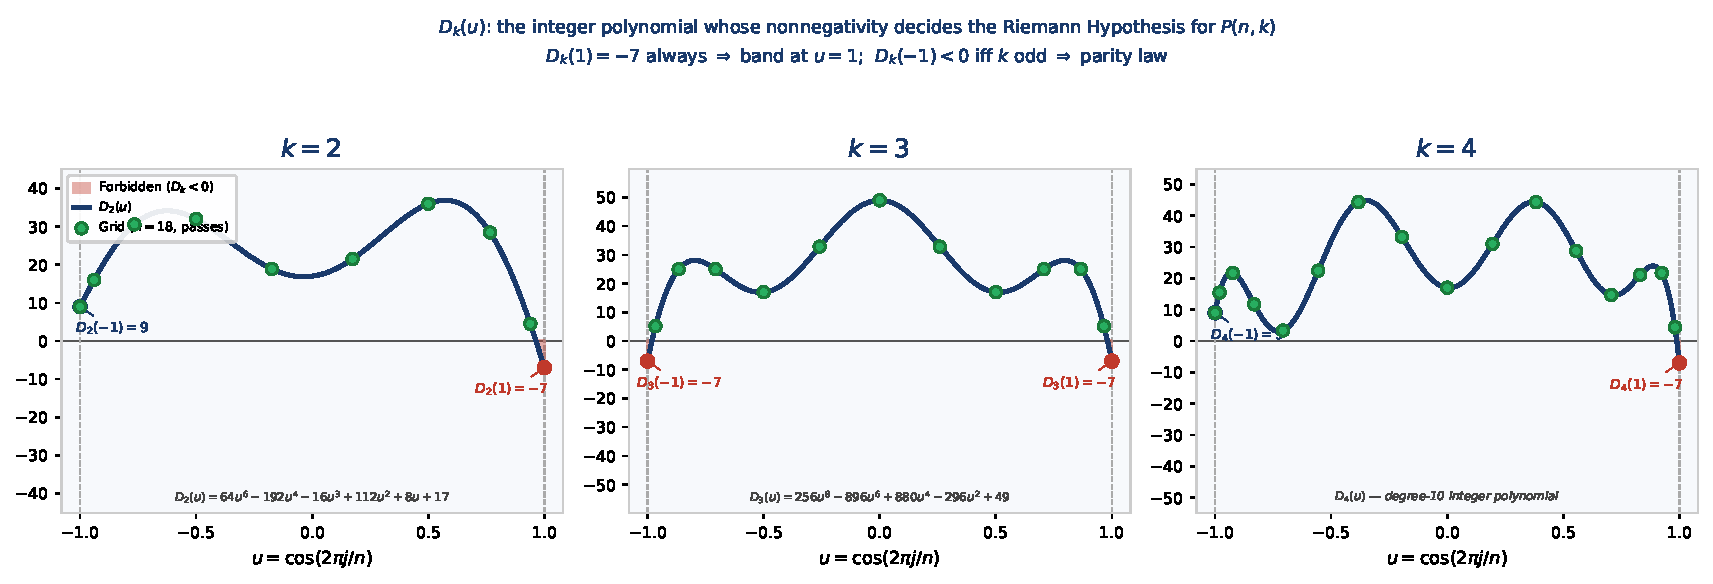
\includegraphics[width=\textwidth]{figures/fig_dk_poly.pdf}
\caption{$D_k(u)$ for $k=2,3,4$ on $[-1,1]$. $D_k(1)=-7$ always, so there is a forbidden band at $u=1$ that a fine grid cannot avoid; $D_k(-1)=-7$ for odd $k$ (a second band at $u=-1$) and $+9$ for even $k$ (no band). Grid points $u_j=\cos(2\pi j/n)$ must all land where $D_k\ge0$.}
\label{fig:dk}
\end{figure}

\begin{thmbox}{Lemma 12.4: Signs at the ends}
$D_k(1)=-7$; $D_k(0)\in\{17,49\}$; $D_k(-1)=-7$ for odd $k$ and $9$ for even $k$. (From $T_k(1)=1$, $T_k(0)\in\{0,\pm1\}$, $T_k(-1)=(-1)^k$.) So $D_k$ has a root in $(0,1)$, and for odd $k$ also one in $(-1,0)$.
\end{thmbox}

\subsection{The Criterion Without $k$: the Corner Criterion}

\begin{thmbox}{Theorem 12.5: Corner criterion}
Put $x=\cos\frac{\pi j(k+1)}{n}$, $y=\cos\frac{\pi j(k-1)}{n}$, and
\begin{equation}
  Q(x,y)=4x^2+4y^2-8\sqrt2\,|xy|+3 .
\end{equation}
Both eigenvalues of $M_j$ lie in $[-2\sqrt2,2\sqrt2]$ if and only if $Q(x,y)\ge0$. The form $Q$ does not involve $k$: $k$ survives only in the map $j\mapsto(x,y)$.
\end{thmbox}

\begin{defbox}{Derivation}
$D_k=(7+P)^2-8A^2$ is a difference of squares: $D_k=f_-f_+$ with $f_\pm=7+P\pm2\sqrt2A$. Both factors cannot be negative at once, because $f_-+f_+=2(7+P)\ge6$; so $D_k\ge0\iff\min(f_-,f_+)\ge0\iff7+P-2\sqrt2|A|\ge0$. Now the product-to-sum identities: $A=\alpha+\beta=2\cos\theta+2\cos k\theta=4\cos\frac{(k+1)\theta}{2}\cos\frac{(k-1)\theta}{2}=4xy$ and $P=\alpha\beta=2\cos(k+1)\theta+2\cos(k-1)\theta=2(2x^2-1)+2(2y^2-1)=4x^2+4y^2-4$, with $\theta=2\pi j/n$. Substituting: $7+4x^2+4y^2-4-8\sqrt2|xy|=Q(x,y)$. \qedhere
\end{defbox}

\begin{figure}[htbp]
\centering
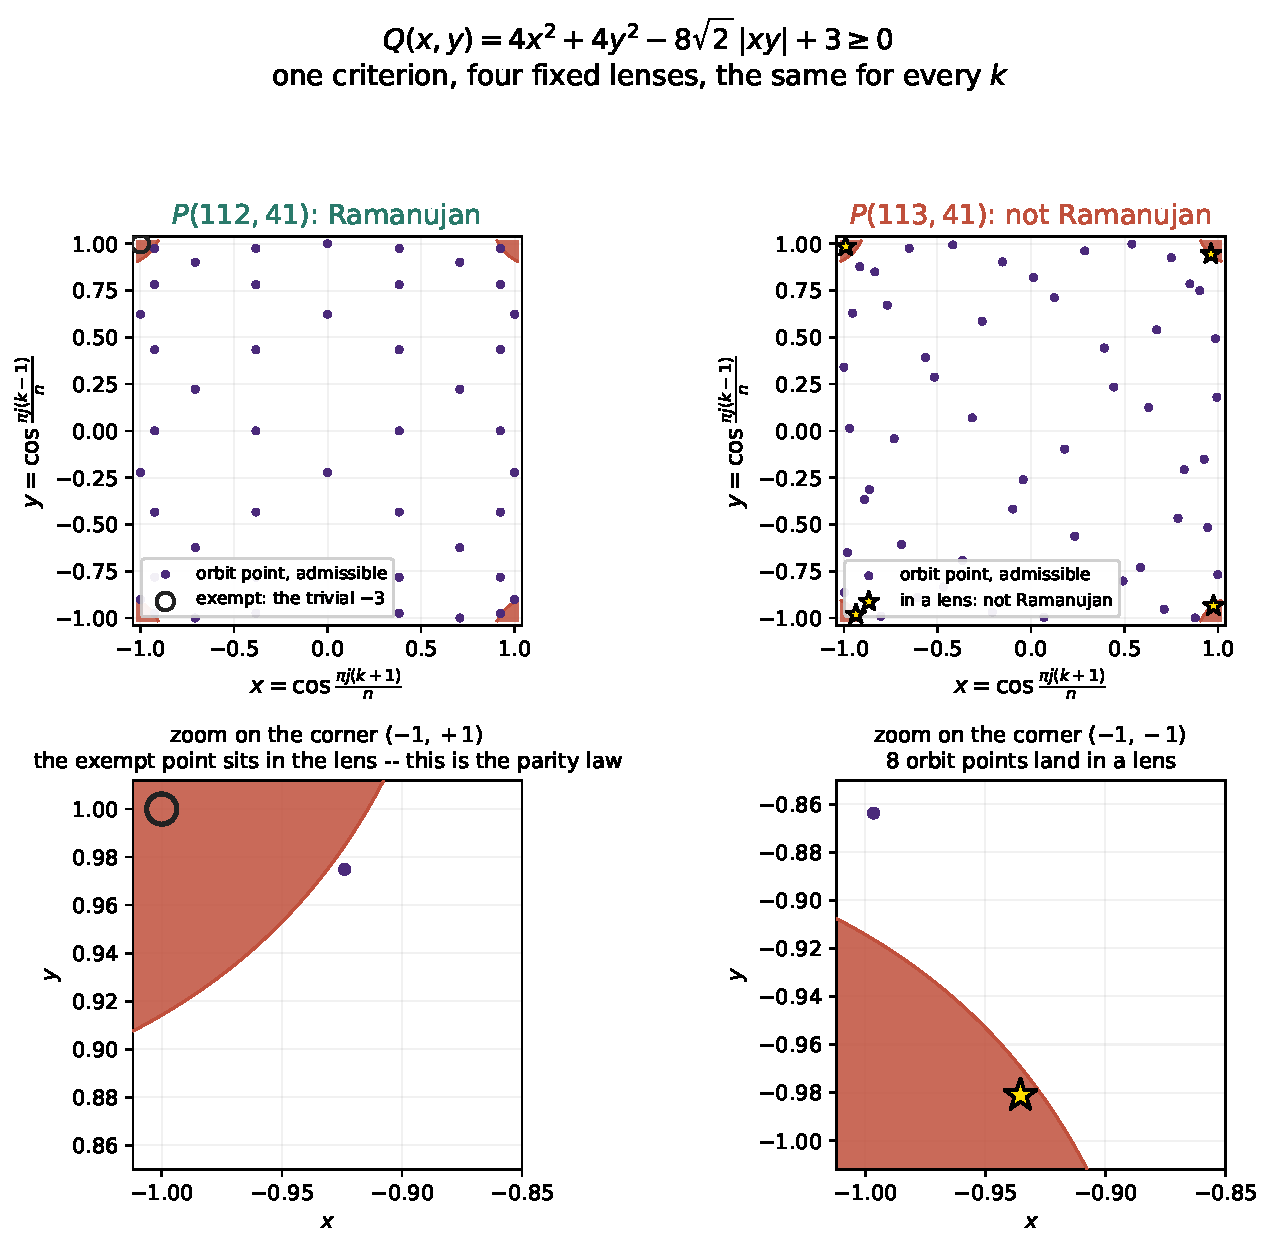
\includegraphics[width=0.9\textwidth]{figures/fig_corner.pdf}
\caption{The corner criterion. The forbidden set $Q<0$ is four congruent lenses at the corners of $[-1,1]^2$, the same for every $k$; together they cover $0.432\%$ of the square. Top: the orbit points $(x,y)$ for $P(112,41)$ (Ramanujan, every point outside the lenses) and $P(113,41)$ (not). Bottom: zooms on the corner lens, showing the one exempt point (the bipartite $-3$, the parity law) and a point that lands inside.}
\label{fig:corner}
\end{figure}

\begin{callbox}{Worked Numerical Example 12.3: The same two verdicts through $Q$}
\begin{itemize}[leftmargin=*,nosep]
  \item $(n,k,j)=(5,2,1)$: $x=\cos(3\pi/5)=-0.30902$, $y=\cos(\pi/5)=0.80902$. $Q=4(0.0955)+4(0.6545)-8\sqrt2(0.25)+3=0.382+2.618-2.828+3=3.172>0$. Agrees with $D_2=28>0$.
  \item $(24,2,1)$: $x=\cos(3\pi/24)=\cos22.5^\circ=0.92388$, $y=\cos(\pi/24)=0.99144$. $Q=3.4142+3.9319-10.3631+3=-0.0170<0$. Agrees with $D_2=-0.3524<0$. The point $(0.924,0.991)$ sits inside the upper-right lens.
\end{itemize}
The lens area: each corner piece has absolute area $\tfrac32-\sqrt2+\tfrac38\log\frac{1+\sqrt2}{3}=0.004322$, and the square $[-1,1]^2$ has area $4$, so the four lenses together cover $4\times0.004322/4=0.432\%$ of it.
\end{callbox}

\subsection{Finiteness Three Ways}

\begin{thmbox}{Theorem 12.6: Per-$k$ finiteness, and uniform finiteness}
Let $u_k$ be the largest root of $D_k$ in $(-1,1)$ and $B_k=2\pi/\arccos u_k$. If $P(n,k)$ is Ramanujan then $n\le B_k$. Moreover, uniformly,
\begin{equation}
  n\ \le\ \pi\bigl(2+\sqrt2\bigr)\sqrt{k^2+1},
\end{equation}
and if $k$ and $n$ are both odd, $n\le\tfrac12\pi(2+\sqrt2)\sqrt{k^2+1}$ (the \textbf{parity law}).
\end{thmbox}

\begin{defbox}{Why: the band at $u=1$ and a grid that is too fine}
$D_k(1)=-7<0$, so $D_k<0$ on $(u_k,1]$. The grid's nonzero point nearest $u=1$ is $u_1=\cos(2\pi/n)$; if $n>B_k$ then $2\pi/n<\arccos u_k$, so $u_1>u_k$ and $D_k(u_1)<0$: the index $j=1$ fails. For the uniform bound one shows, with $s=(1-\cos t)+(1-\cos kt)$ and $\tau=3-2\sqrt2$, that $s<\tau$ already forces failure (AM--GM on the two pieces of $7+P-2\sqrt2|A|$), and $1-\cos\theta\le\theta^2/2$ gives $s\le(1+k^2)t^2/2$; at $t=2\pi/n$ this is $<\tau$ once $n>\pi(2+\sqrt2)\sqrt{k^2+1}$. For odd $k$ the band at $u=-1$ is also present; odd $n$ has a grid point at distance $\pi/n$ from $\pi$ --- half the distance --- while even $n$ hits $\pi$ exactly at the exempt index $j=n/2$. Bipartiteness helps.
\end{defbox}

\begin{callbox}{Worked Numerical Example 12.4: The uniform bound at $k=2,3$}
$k=2$: $\pi(2+\sqrt2)\sqrt5=10.726\cdot2.236=23.98$, so $n\le23$. Sharp: $P(23,2)$ is Ramanujan and $P(24,2)$ is not (Example 12.2). $k=3$: $\pi(2+\sqrt2)\sqrt{10}=33.9$, so $n\le33$; the actual last member is $n=32$ ($B_3=32$). The per-$k$ bound $B_k$ is exact by construction; the uniform one is what it says, uniform.
\end{callbox}

\begin{thmbox}{Theorem 12.7: Absolute finiteness (Dirichlet)}
If $n\ge231$ then $P(n,k)$ fails the Riemann Hypothesis for \emph{every} $k$. Hence the whole family is finite in both variables.
\end{thmbox}

\begin{defbox}{Proof}
Failure is forced at index $j$ as soon as $\bigl(1-\cos\frac{2\pi j}{n}\bigr)+\bigl(1-\cos\frac{2\pi jk}{n}\bigr)<\tau$. With $\|\theta\|$ the distance to the nearest integer, $1-\cos2\pi\theta=2\sin^2\pi\theta\le2\pi^2\|\theta\|^2$, so it is enough that
\begin{equation}
  \Bigl\|\tfrac jn\Bigr\|^2+\Bigl\|\tfrac{jk}{n}\Bigr\|^2<\frac{\tau}{2\pi^2}=0.0086919\ldots
\end{equation}
Let $J=\lfloor\sqrt n\rfloor$. \textbf{Dirichlet's approximation theorem} gives an integer $1\le j\le J$ with $\|jk/n\|\le1/(J+1)$. For it, $\|j/n\|^2\le(J/n)^2\le1/n$ and $\|jk/n\|^2\le1/(J+1)^2<1/n$, so the left side is $<2/n$. Hence $2/n<\tau/(2\pi^2)$ suffices, i.e.\ $n>4\pi^2/\tau=230.097\ldots$ The index is legitimate: $1\le j\le\sqrt n<n/2$ for $n\ge5$. \qedhere
\end{defbox}

\begin{callbox}{Worked Numerical Example 12.5: Dirichlet at $n=231$, $k=100$}
$J=\lfloor\sqrt{231}\rfloor=15$. Among $j=1,\dots,15$ the best is $j=7$: $7\cdot100/231=3.0303$, so $\|jk/n\|=0.0303\le1/16=0.0625$. Then $\|j/n\|^2+\|jk/n\|^2=(7/231)^2+0.0303^2=0.000918+0.000918=0.001837<0.008692$. So $P(231,100)$ fails at $j=7$, without computing a single eigenvalue. The threshold $231$ is not sharp (nothing survives past $n=\RamAllMaxN$); its only job is to be independent of $k$.
\end{callbox}

\subsection{The Complete Classification}

\begin{thmbox}{Theorem 12.8: Complete classification}
Exactly $\RamAllTotal$ pairs $(n,k)$ with $n\ge3$, $1\le k<n/2$ satisfy the Riemann Hypothesis; they fall into $\RamAllIso$ isomorphism classes (since $P(n,k)\cong P(n,\ell)$ iff $\ell\equiv\pm k^{\pm1}\bmod n$). The largest is $n=\RamAllMaxN$ at $k=41$; the largest $k$ is $\RamAllMaxK$; the $k$ that occur are $1,\dots,25$ and the odd numbers from $27$ to $\RamAllMaxK$. All $\RamAllCases$ cases in the region $3\le n\le230$ were decided in exact arithmetic.
\end{thmbox}

\begin{figure}[htbp]
\centering
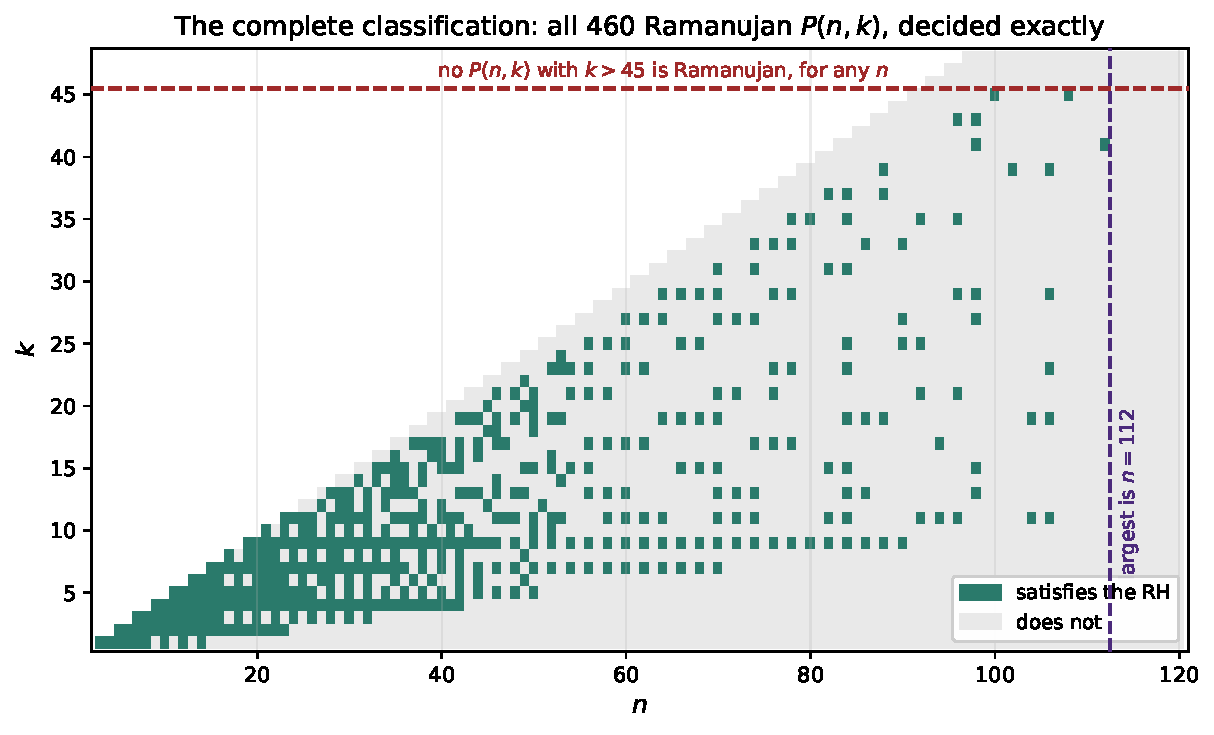
\includegraphics[width=0.85\textwidth]{figures/fig_ramclass.pdf}
\caption{The classification: every $(n,k)$ with $P(n,k)$ Ramanujan. Nothing past $n=112$; nothing with $k>45$; above $k=25$ only odd $k$, the parity law still operating at the end of the list.}
\label{fig:ramclass}
\end{figure}

\begin{table}[htbp]
\centering\footnotesize
% GENERATED by verification/verify_all.py -- do not edit by hand.
\begin{tabular}{r r r l}
\hline
$k$ & $B_k$ & count & the $n$ for which $P(n,k)$ satisfies the RH\\
\hline
$1$ & $15$ & $9$ & $3\text{--}8, 10, 12, 14$\\
$2$ & $23$ & $19$ & $5\text{--}23$\\
$3$ & $32$ & $18$ & $7\text{--}16, 18, 20, 22, 24, 26, 28, 30, 32$\\
$4$ & $42$ & $34$ & $9\text{--}42$\\
$5$ & $51$ & $28$ & $11\text{--}26, 28, 30, 32, 34, 36, 38, 40, 42, 44, 46, 48, 50$\\
$6$ & $61$ & $20$ & $13\text{--}16, 18, 20\text{--}23, 25, 27\text{--}28, 30, 32, 35, 37, 39, 42, 44, 49$\\
$7$ & $71$ & $39$ & $15\text{--}36, 38, 40, 42, 44, 46, 48, 50, 52, 54, 56, 58, 60, 62, 64, 66, 68, 70$\\
$8$ & $81$ & $16$ & $17, 19\text{--}22, 24, 26, 28\text{--}29, 31, 33, 35, 38, 40, 42, 49$\\
$9$ & $91$ & $50$ & $19\text{--}46, 48, 50, 52, 54, 56, 58, 60, 62, 64, 66, 68, 70, 72, 74, 76, 78, 80, 82, 84, 86, 88, 90$\\
$10$ & $101$ & $14$ & $21, 23, 25\text{--}26, 28, 30, 32, 34, 37, 39, 41, 43, 50, 52$\\
$11$ & $111$ & $36$ & $23\text{--}26, 28\text{--}32, 35\text{--}38, 40\text{--}42, 46\text{--}48, 50, 52\text{--}53, 58, 60, 62, 64, 70, 72, 74, 82, 84, 92, 94, 96, 104, 106$\\
$12$ & $121$ & $9$ & $27, 29\text{--}30, 32, 34, 38, 40, 45, 51$\\
$13$ & $131$ & $23$ & $28\text{--}30, 32, 34\text{--}37, 42\text{--}44, 46, 48\text{--}49, 56, 58, 60, 70, 72, 74, 84, 86, 98$\\
$14$ & $141$ & $7$ & $31, 33, 35\text{--}36, 38, 46, 53$\\
$15$ & $151$ & $19$ & $33\text{--}36, 38, 40\text{--}42, 49\text{--}50, 52, 54, 56, 66, 68, 70, 82, 84, 98$\\
$16$ & $161$ & $6$ & $35, 39\text{--}40, 42, 44, 52$\\
$17$ & $171$ & $16$ & $37\text{--}40, 42, 44, 46\text{--}47, 56, 58, 60, 62, 74, 76, 78, 94$\\
$18$ & $181$ & $3$ & $45\text{--}46, 50$\\
$19$ & $191$ & $17$ & $42\text{--}44, 46, 48, 50, 52\text{--}53, 64, 66, 68, 70, 84, 86, 88, 104, 106$\\
$20$ & $201$ & $3$ & $45, 49\text{--}50$\\
$21$ & $211$ & $11$ & $46, 48, 50, 54, 56, 58, 70, 72, 76, 92, 96$\\
$22$ & $221$ & $1$ & $49$\\
$23$ & $231$ & $10$ & $52\text{--}54, 56, 60, 62, 76, 78, 84, 106$\\
$24$ & $241$ & $1$ & $53$\\
$25$ & $251$ & $8$ & $56, 58, 60, 66, 68, 84, 90, 92$\\
$27$ & $271$ & $8$ & $60, 62, 64, 70, 72, 74, 90, 98$\\
$29$ & $291$ & $9$ & $64, 66, 68, 70, 76, 78, 96, 98, 106$\\
$31$ & $311$ & $4$ & $70, 74, 82, 84$\\
$33$ & $331$ & $5$ & $74, 76, 78, 86, 90$\\
$35$ & $351$ & $5$ & $78, 80, 84, 92, 96$\\
$37$ & $371$ & $3$ & $82, 84, 88$\\
$39$ & $391$ & $3$ & $88, 102, 106$\\
$41$ & $412$ & $2$ & $98, 112$\\
$43$ & $432$ & $2$ & $96, 98$\\
$45$ & $452$ & $2$ & $100, 108$\\
\hline
\multicolumn{4}{l}{\footnotesize No $k$ outside this table admits any $n$: the list is finite in both variables.}\\
\end{tabular}

\caption{The Ramanujan $P(n,k)$ for $k\le25$ (generated by \texttt{verify\_all.py}): $B_k$ is the per-$k$ bound of Theorem 12.6, count the number of $n$, then the list. Note the $k=2$ row is $5$--$23$ as in Example 12.2.}
\label{tab:ram}
\end{table}

\begin{callbox}{How ``decided in exact arithmetic'' works}
On the grid, $A=c_1+c_k$ and $P=c_{k+1}+c_{k-1}$ with $c_r=2\cos(2\pi rj/n)$ are values of integer Laurent polynomials at roots of unity. Reducing modulo the cyclotomic polynomial $\Phi_m$ ($m=n/\gcd(n,j)$) decides whether $Q$ vanishes \emph{exactly}, by integer arithmetic; when it does not vanish, a separation bound for nonzero algebraic integers tells how far from zero it must be, and a high-precision evaluation guarded by that bound decides the sign. A floating-point control runs alongside with no authority: $0$ disagreements across all $\RamAllCases$ cases, and the smallest margin any case was decided on is $6.1\times10^{-5}$, at $(n,k)=(172,72)$.
\end{callbox}

\subsection{A Theorem Instead of a Table: the Closed Form for $k\le9$}

\begin{thmbox}{Theorem 12.8a: Closed form for $k\in\{1,2,3,4,5,7,9\}$}
Let $u_k$ be the largest root of $D_k$ below $1$, $B_k=2\pi/\arccos u_k$ and $P_k=B_k/2$. Then $P(n,k)$ is Ramanujan iff $2k<n\le B_k$, and, when $k$ is odd and $n$ is odd, additionally $n\le P_k$. For $k=6,8$ and every $k\ge10$ this fails: $D_k$ has an interior band.
\end{thmbox}

\begin{intubox}{What makes it a proof}
Two facts. First, where $D_k$ is negative on $[-1,1]$: for these $k$ it is only the end band $(u_k,1]$, plus its mirror image $[-1,-u_k)$ when $k$ is odd (because $D_k$ is then an even polynomial). That is a statement about the real roots of one integer polynomial, and Sturm's theorem decides it in integer arithmetic (\texttt{verification/interior\_bands.py} does the root isolation exactly over $\mathbb Q$; for $k=2$ it fits on a page). Second, which grid points can enter a band: the point closest to $1$ is $j=1$, and the point closest to $-1$ is $j=n/2$ (exempt, the trivial eigenvalue $-3$) when $n$ is even and $j=(n-1)/2$ when $n$ is odd. So failure at even $n$ means $\cos\frac{2\pi}{n}>u_k$, i.e.\ $n>B_k$, and failure at odd $n$ for odd $k$ means $\cos\frac{\pi}{n}>u_k$, i.e.\ $n>B_k/2$.
\end{intubox}

\begin{callbox}{Worked Example 12.8a: $k=3$ by hand}
$u_3=0.9814\ldots$, so $B_3=2\pi/\arccos(0.9814)=32.5$ and $P_3=16.26$. Even $n$: Ramanujan iff $n\le32$. Odd $n$: iff $n\le15$. Check against the census: $k=3$ has $n=7,\dots,16$ and then $18,20,\dots,32$, eighteen values, exactly the even $n\le32$ together with the odd $n\le15$. For $k=6$ the same reasoning would predict an unbroken run up to $B_6=49$, but the list is $13,14,15,16,\dots$ with gaps, because $D_6$ is also negative on $(-0.895,-0.846)$ and grid points fall into that interior band.
\end{callbox}

\subsection{Structure of the List: Locality}

\begin{thmbox}{Theorem 12.9: Locality at divisors}
Call $m=n/\gcd(n,j)$ the \emph{level} of index $j$, and say $m$ is \emph{bad for $k$} if some primitive level-$m$ point violates $Q\ge0$. Then $P(n,k)$ is Ramanujan if and only if no divisor $m\ge3$ of $n$ is bad for $k$, and badness at level $m$ depends on $k$ only through $k\bmod m$. Consequently the Ramanujan set of each $k$ is closed under taking divisors $d>2k$ of $n$.
\end{thmbox}

\begin{intubox}{Intuition}
The grid point $\cos(2\pi j/n)$ ``is'' a primitive $m$th cosine, and all the primitive $m$th cosines are Galois conjugate --- they come together. So the criterion only ever looks at one level at a time, and a level is bad or good for $k$ depending only on $k$ modulo $m$. This is why the list in Table~\ref{tab:ram} has so much repetition in its tails (the $n$ that survive at large $k$ are those all of whose divisors are ``safe''), and it gives a cheap sufficient test: if $m/\gcd(k\pm1,m)\in\{2,\dots,7\}$ then $m$ is safe for $k$ (Theorem \emph{gcdsafe} of the paper). A closed form was not found; the paper says exactly where the attempt stops.
\end{intubox}

\subsection{Every Cubic Cyclic Cover, and the No-Go}

\begin{thmbox}{Theorem 12.10: The two cubic two-vertex bases}
A cubic cover of a two-vertex base is either $B(a,b,c)^n$ --- loops of voltages $a$ at $u$ and $b$ at $v$, an edge of voltage $c$ --- or a theta base $T(c_1,c_2,c_3)^n$ with three parallel edges (a cubic cyclic Haar graph, bipartite). $P(n,k)=B(1,k,0)^n$.
\begin{itemize}[leftmargin=*,nosep]
  \item $B(a,b,c)^n$ is Ramanujan iff $Q\bigl(\cos\frac{\pi j(a+b)}{n},\cos\frac{\pi j(a-b)}{n}\bigr)\ge0$ at every nontrivial $j$ --- the \emph{same} $Q$ with $(a+b,a-b)$ in place of $(k+1,k-1)$; the edge voltage $c$ plays no role.
  \item $T(c_1,c_2,c_3)^n$ is Ramanujan iff $\sum_{l<m}\cos\frac{2\pi j(c_l-c_m)}{n}\le\frac52$ for every $j\ne0$.
\end{itemize}
\end{thmbox}

\begin{callbox}{Worked Numerical Example 12.6: The theta base $T(0,1,2)$}
The block is $\begin{psmallmatrix}0&S_j\\\overline{S_j}&0\end{psmallmatrix}$ with $S_j=1+\omega^j+\omega^{2j}$, eigenvalues $\pm|S_j|$, and $|S_j|^2=3+2\bigl(\cos\tfrac{2\pi j}{n}+\cos\tfrac{2\pi j}{n}+\cos\tfrac{4\pi j}{n}\bigr)$. Ramanujan needs $|S_j|^2\le8$ for $j\ne0$. The uniform bound is $n\le2\pi\sqrt{d_1^2+d_2^2+d_3^2}=2\pi\sqrt{1+1+4}=2\pi\sqrt6=15.39$, and $n=15$ is in fact Ramanujan: the bound is attained.
\end{callbox}

\begin{thmbox}{Theorem 12.11: No infinite Ramanujan family is a cyclic cover}
Let $B$ be a fixed connected cubic base with integer voltages, $L=\sqrt2\sum|v_e|$ over non-loop edges and $R=\sum v_e^2$ over loops. Then $B^n$ is not Ramanujan as soon as $\frac{2\pi}{n}L+\bigl(\frac{2\pi}{n}\bigr)^2R<3-2\sqrt2$. In particular only finitely many $n$ qualify.
\end{thmbox}

\begin{defbox}{Proof (Weyl's inequality)}
$M_0$ is the adjacency matrix of the base, $3$-regular, top eigenvalue $3$. Each entry of $M_1$ differs from the corresponding entry of $M_0$ by at most $|\omega^v-1|\le2\pi|v|/n$ (non-loop edge) or $|2\cos\frac{2\pi v}{n}-2|\le(2\pi v/n)^2$ (loop); summing, $\|M_1-M_0\|_2\le\frac{2\pi}{n}L+(\frac{2\pi}{n})^2R$. By Weyl, $\lambda_{\max}(M_1)\ge3-\|M_1-M_0\|_2$, and $\lambda_{\max}(M_1)$ is nontrivial because $3$ is simple in a connected cover and lives at $j=0$. So once the displayed quantity is below $3-2\sqrt2$, a nontrivial eigenvalue exceeds $2\sqrt2$. \qedhere
\end{defbox}

\begin{intubox}{What this is, and is not}
It is the cyclic instance of the known principle that abelian covers do not expand --- which is why the Lubotzky--Phillips--Sarnak Ramanujan graphs are built on $\mathrm{PGL}_2$, not on a cyclic group. The paper claims no novelty for the principle; what is new is the explicit constant and the two exact criteria that decide the finitely many survivors.
\end{intubox}

\subsection{The Deficit: What the No-Go Costs}

\begin{defbox}{Definition 12.3}
For a cover with nontrivial spectral radius $\lambda_2$, the \textbf{deficit} is $\delta=\lambda_2-2\sqrt2$; for a size $n$, $\delta^\ast(n)=\min_{1\le k<n/2}\delta(n,k)$. $\delta^\ast(n)\le0$ exactly when some $P(n,k)$ is Ramanujan, which happens for $\RamAllSizes$ values of $n$, the largest $\RamAllMaxN$.
\end{defbox}

\begin{thmbox}{Proposition 12.12}
$\delta(n,k)<3-2\sqrt2=0.1716\ldots$ for every $n,k$, and the supremum is exactly $3-2\sqrt2$, approached as $n\to\infty$. (Because $\lambda_2<3$, $3$ being simple; and at $j=1$, $M_1\to M_0$, whose top eigenvalue is $3$.)
\end{thmbox}

\begin{callbox}{Worked Numerical Example 12.7}
$P(24,2)$: $\lambda_2=2.8369$, so $\delta=0.0085$ --- it misses the threshold by less than a hundredth. An engineer forced to build at a size with no optimal member gives up at most $0.1716$ in nontrivial spectral radius, and the typical loss is far smaller (Figure~\ref{fig:deficit}).
\end{callbox}

\begin{figure}[htbp]
\centering
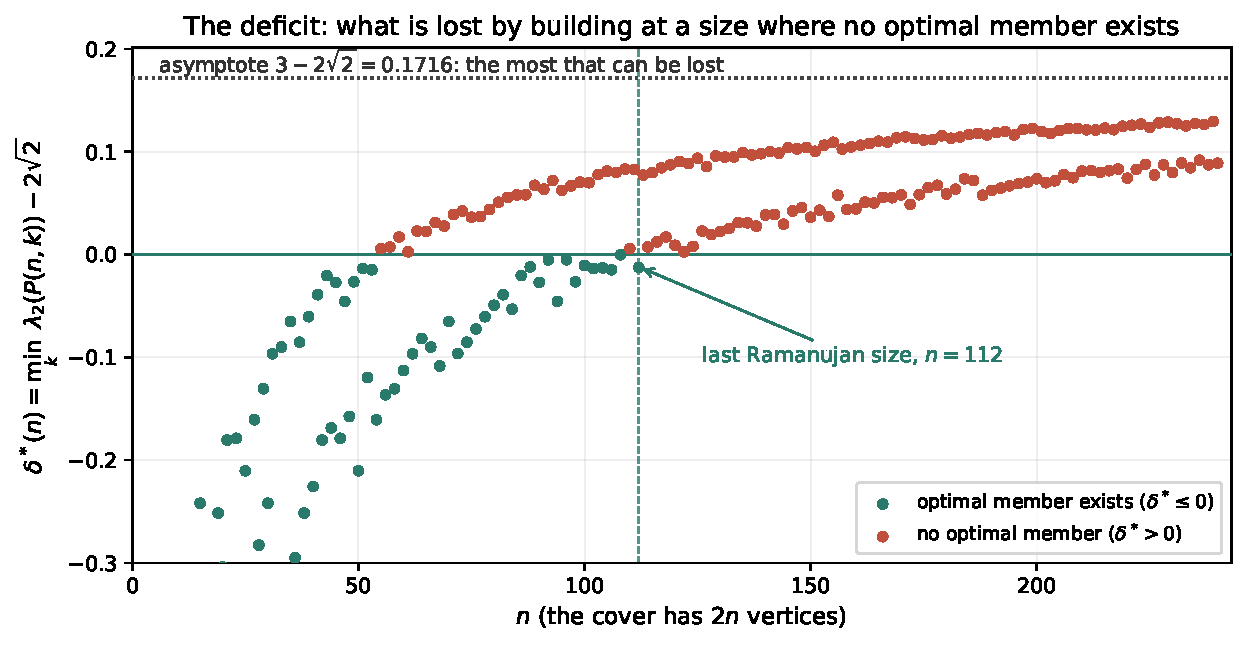
\includegraphics[width=0.9\textwidth]{figures/fig_deficit.pdf}
\caption{$\delta^\ast(n)$: the best achievable nontrivial spectral radius at each size, measured from $2\sqrt2$. Green: sizes with a Ramanujan member (last at $n=112$). The curve rises towards the asymptote $3-2\sqrt2$; the two branches are the parity law.}
\label{fig:deficit}
\end{figure}

\newpage
%% =========================================================================
%% SECTION 13: VERIFICATION -- WHAT "CERTIFIED" MEANS HERE
%% =========================================================================
\section{Verification: What ``Certified'' Means in This Project}

\begin{defbox}{The four standards, in decreasing strength}
\begin{enumerate}[leftmargin=*,nosep]
  \item \textbf{Proved}: a proof in the text.
  \item \textbf{Proved by an exact certificate}: an explicit matrix whose nullity is computed in $\mathbb Z$, $\mathbb Q$ or a cyclotomic field --- integer Gaussian elimination, no rounding anywhere.
  \item \textbf{Proved by interval certification}: a Krawczyk contraction bound (Section 9) establishing that a true real solution exists in an explicit box, with the bound itself evaluated in exact rational arithmetic.
  \item \textbf{Numerical}: a floating-point computation only. Reported, labelled, and never used as a premise.
\end{enumerate}
\end{defbox}

\begin{callbox}{The suite: \texttt{verification/verify\_all.py}}
One script re-derives every computational claim in the paper --- $\Nchecks$ checks, each printing PASS or FAIL with the quantity it measured --- in about seven minutes. Its rules:
\begin{itemize}[leftmargin=*,nosep]
  \item \textbf{Nothing is taken on trust from a stored file.} Saved certificates are re-evaluated, not believed.
  \item \textbf{Exact arithmetic wherever a decision is made.} A floating-point control runs alongside; it has no authority, and if the two disagree the run \emph{fails} rather than picking a winner.
  \item \textbf{Every number in the manuscript is generated, not typed.} The file \texttt{zf\_numbers.tex} (tile counts, thresholds, the $\RamAllTotal$, $\Nchecks$ itself) is written by the suite from the certificates on disk; the paper, the board and this guide read it. A stale number fails the build before it reaches a reader.
  \item \textbf{Controls that can fire.} Where a new bound is introduced, the suite asserts it against every existing certificate: the period-one ceiling of Section 11, for instance, is checked to be $\ge2k+2$ at all $16$ pairs $(n,k)$ where a period-one certificate of nullity $2k+2$ exists. If that ever failed, the argument would be wrong and the run would say so.
\end{itemize}
\end{callbox}

\begin{callbox}{What it caught (claims of ours that were wrong)}
\begin{itemize}[leftmargin=*,nosep]
  \item A float64 guard in the exact Ramanujan classifier underflowed to $0$ for $n>126$, so one test could never pass; found when the suite's control disagreed.
  \item A ``strict gap'' $M(P(10,2))<Z$ reported by an optimiser: two more seeds found nullity $6$ (Section 11.4 now certifies it).
  \item A search objective (sum of the $d$ smallest squared singular values) that reports success when one value is $10^{-10}$ and the rest $10^{-6}$ --- it produced a false counterexample, caught by recomputing the rank exactly.
  \item A false \emph{negative}: an adversarial search that found nothing on the star-with-a-loop base was written into the paper as evidence for the cover ceiling; the counterexample (Theorem 10.4) was then found by reasoning about pendant vertices.
\end{itemize}
\end{callbox}

\begin{callbox}{What it did not catch, and who did}
The suite checks arithmetic. It does not check whether a theorem is stated with the right hypotheses. Theorem 10.1 was stated without ``$\det M(\zeta)\not\equiv0$'' and the suite could not object, because every matrix it was handed satisfied the hypothesis. The error was found by an outside reader of a one-page summary, who asked what the voltages of the $K_4$ base actually were and noticed a triangle. Two adversarial searches had passed over the same matrix. The honest answer to ``how do you check the assisted work?'' is therefore: the suite catches what can be computed; inconsistency between what is claimed and what is used is caught by reading --- by a second method, not a more careful first one.
\end{callbox}

\newpage
\section{Complete Step-by-Step Worked Numerical Examples}

To make every single formula in this guide completely concrete, we carry out all calculations by hand on three explicit examples.

\subsection{Example 1: Complete Hand-Worked Derivation on $P(6,2)$}

Let $G = P(6,2)$. This is a cubic graph on $2n = 12$ vertices:
\begin{itemize}[leftmargin=*,nosep]
  \item Vertices: Outer ring $\{u_0, u_1, \dots, u_5\}$; Inner ring $\{v_0, v_1, \dots, v_5\}$.
  \item Outer edges ($u_i u_{i+1}$): $(u_0, u_1), (u_1, u_2), (u_2, u_3), (u_3, u_4), (u_4, u_5), (u_5, u_0)$.
  \item Spoke edges ($u_i v_i$): $(u_0, v_0), (u_1, v_1), (u_2, v_2), (u_3, v_3), (u_4, v_4), (u_5, v_5)$.
  \item Inner edges ($v_i v_{i+2}$): $(v_0, v_2), (v_2, v_4), (v_4, v_0)$ and $(v_1, v_3), (v_3, v_5), (v_5, v_1)$.
\end{itemize}
Notice that $\gcd(6, 2) = 2$. As predicted by the Clock Lemma (Theorem 1.1), the inner ring splits into \textbf{two disjoint triangles}: $\{v_0, v_2, v_4\}$ and $\{v_1, v_3, v_5\}$.

\noindent\textbf{Step 1: Running Zero Forcing by Hand.}
Choose $S = \{u_0, u_1, u_2, u_3, u_4, u_5\}$ (all 6 outer vertices).
\begin{itemize}[leftmargin=*,nosep]
  \item Examine $u_0$: Its neighbours are $u_5$ (black), $u_1$ (black), and $v_0$ (white).
  Exactly one white neighbour. $u_0 \to v_0$ forces $v_0$ black.
  \item By identical reasoning, each $u_i \to v_i$ forces $v_i$ black.
  \item After 1 round, all 12 vertices are black. Thus $Z(P(6,2)) \le 6$.
\end{itemize}

\noindent\textbf{Step 2: Checking the Bootstrap Hypothesis.}
Theorem 4.1 requires $n \ge 2(j+k) + 1 = 2(1+2) + 1 = 7$.
Here $n = 6 < 7$. The hypothesis is not met. 
Indeed, $u_{2(j+k)} = u_6 \equiv u_0 \pmod 6$, which was already in $S$. The bootstrap chain degenerates on small $n$, proving why the inequality $n \ge 2k+3$ is strictly necessary.

\noindent\textbf{Step 3: Calculating Fourier Blocks and Chebyshev Polynomials.}
For $n=6, k=2$, we compute the double cosines $s_m = 2\cos(2\pi m / 6)$ and $t_m = 2\cos(4\pi m / 6)$:
\begin{center}
\begin{tabular}{c|cccccc}
\toprule
$m$ & 0 & 1 & 2 & 3 & 4 & 5 \\
\midrule
$s_m = 2\cos(2\pi m / 6)$ & 2 & 1 & $-1$ & $-2$ & $-1$ & 1 \\
$t_m = 2\cos(4\pi m / 6)$ & 2 & $-1$ & $-1$ & 2 & $-1$ & $-1$ \\
\bottomrule
\end{tabular}
\end{center}
Check the Chebyshev identity $L_2(s) = s^2 - 2$:
\begin{itemize}[leftmargin=*,nosep]
  \item For $m=1$: $s_1 = 1 \implies L_2(1) = 1^2 - 2 = -1 = t_1$. \checkmark
  \item For $m=3$: $s_3 = -2 \implies L_2(-2) = (-2)^2 - 2 = 2 = t_3$. \checkmark
\end{itemize}
The distinct grid values in $\Gamma_6$ are $\{2, 1, -1, -2\}$ (only 4 points.).
Suppose we choose roots $\{1, -1, -2\}$. The target cubic is:
\begin{equation}
  (s - 1)(s + 1)(s + 2) = s^3 + 2s^2 - s - 2.
\end{equation}
Matching coefficients with $F(s) = (s+a)(s^2-2) + \alpha s + \beta = s^3 + a s^2 + (\alpha - 2) s + (\beta - 2a)$:
\begin{align}
  a &= 2, \\
  \alpha - 2 &= -1 \implies \alpha = 1, \\
  \beta - 2(2) &= -2 \implies \beta = 2.
\end{align}
Now check admissibility:
\begin{equation}
  c^2 = a\alpha - \beta = (2)(1) - 2 = \mathbf{0}.
\end{equation}
$c^2 = 0$ is inadmissible. Spoke weight zero disconnects the graph. 
This hand calculation proves exactly why $n=6$ fails to host an equivariant certificate, matching our theoretical degeneracy analysis.

\noindent\textbf{Step 4: Explicit Adjacency Matrix, Fourier Blocks, and Spectrum.}
Let us write out the unweighted adjacency matrix of $P(6,2)$ in block form:
\begin{equation}
  A = \begin{pmatrix} U & I_6 \\ I_6 & V \end{pmatrix},
\end{equation}
where $U$ is the outer 6-cycle and $V$ is the inner chord matrix:
\begin{equation}
  U = \begin{pmatrix}
    0 & 1 & 0 & 0 & 0 & 1 \\
    1 & 0 & 1 & 0 & 0 & 0 \\
    0 & 1 & 0 & 1 & 0 & 0 \\
    0 & 0 & 1 & 0 & 1 & 0 \\
    0 & 0 & 0 & 1 & 0 & 1 \\
    1 & 0 & 0 & 0 & 1 & 0
  \end{pmatrix}, \qquad
  V = \begin{pmatrix}
    0 & 0 & 1 & 0 & 1 & 0 \\
    0 & 0 & 0 & 1 & 0 & 1 \\
    1 & 0 & 0 & 0 & 1 & 0 \\
    0 & 1 & 0 & 0 & 0 & 1 \\
    1 & 0 & 1 & 0 & 0 & 0 \\
    0 & 1 & 0 & 1 & 0 & 0
  \end{pmatrix}.
\end{equation}
Now compute the 6 uncoupled $2 \times 2$ Fourier blocks $M_m = \begin{pmatrix} s_m & 1 \\ 1 & t_m \end{pmatrix}$:
\begin{align}
  M_0 &= \begin{pmatrix} 2 & 1 \\ 1 & 2 \end{pmatrix} \implies \det M_0 = (2)(2) - 1 = \mathbf{3} \ne 0, \\
  M_1 &= \begin{pmatrix} 1 & 1 \\ 1 & -1 \end{pmatrix} \implies \det M_1 = (1)(-1) - 1 = \mathbf{-2} \ne 0, \\
  M_2 &= \begin{pmatrix} -1 & 1 \\ 1 & -1 \end{pmatrix} \implies \det M_2 = (-1)(-1) - 1 = \mathbf{0} \quad \text{(\textbf{SINGULAR.})}, \\
  M_3 &= \begin{pmatrix} -2 & 1 \\ 1 & 2 \end{pmatrix} \implies \det M_3 = (-2)(2) - 1 = \mathbf{-5} \ne 0, \\
  M_4 &= \begin{pmatrix} -1 & 1 \\ 1 & -1 \end{pmatrix} \implies \det M_4 = (-1)(-1) - 1 = \mathbf{0} \quad \text{(\textbf{SINGULAR.})}, \\
  M_5 &= \begin{pmatrix} 1 & 1 \\ 1 & -1 \end{pmatrix} \implies \det M_5 = (1)(-1) - 1 = \mathbf{-2} \ne 0.
\end{align}
Notice that blocks $M_2$ and $M_4$ are singular. 
For $M_2$, $M_2 \begin{pmatrix} 1 \\ 1 \end{pmatrix} = \begin{pmatrix} -1+1 \\ 1-1 \end{pmatrix} = \begin{pmatrix} 0 \\ 0 \end{pmatrix}$.
Each singular block has nullity 1, so the full $12 \times 12$ adjacency matrix has nullity:
\begin{equation}
  \operatorname{null}(\operatorname{Adj} P(6,2)) = 1 + 1 = \mathbf{2}.
\end{equation}
Now check our Conway--Jones classification formula (Theorem 8.2):
$P_2(z) = \Phi_3(z) \Phi_{10}(z)$.
The cyclotomic divisors are $d \in \{3, 10\}$.
Which of these divide $n=6$? Only $d=3$ divides $6$ ($6/3 = 2$).
Theorem 8.2 predicts:
\begin{equation}
  \operatorname{null}(\operatorname{Adj} P(6,2)) = \varphi(3) = \mathbf{2}.
\end{equation}
The formula matches the explicit block calculation with 100\% agreement.

\subsection{Example 2: Exact Integer Certificate on $P(30,2)$}

Now take $n=30, k=2$. Here $30 \ge 2k+3 = 7$, and $30 \mid n$.
From Table~\ref{tab:cyclotomic}, we use cyclotomic factors $D = \{3, 10\}$:
\begin{equation}
  F(s) = \Psi_3(s) \Psi_{10}(s) = (s + 1)(s^2 - s - 1) = s^3 - 2s - 1.
\end{equation}
Compare with $F(s) = (s+a)(s^2-2) + \alpha s + \beta = s^3 + a s^2 + (\alpha - 2) s + (\beta - 2a)$:
\begin{align}
  a &= 0, \\
  \alpha - 2 &= -2 \implies \alpha = 0, \\
  \beta - 0 &= -1 \implies \beta = -1.
\end{align}
Admissibility check:
\begin{equation}
  c^2 = a\alpha - \beta = (0)(0) - (-1) = \mathbf{1} > 0. \quad \text{(\textbf{Admissible.})}
\end{equation}
Thus $a=0, d=0, c=1$: The certificate is the \textbf{unweighted integer adjacency matrix}.
Let us identify the 6 roots of $F(s)$ on the grid $\Gamma_{30}$:
\begin{itemize}[leftmargin=*,nosep]
  \item Factor $\Psi_3(s) = s + 1 = 0 \implies s = -1$.
  $2\cos(2\pi m / 30) = -1 \iff 2\pi m / 30 = \pm 2\pi/3 \iff m \in \{10, 20\}$. (2 roots.)
  \item Factor $\Psi_{10}(s) = s^2 - s - 1 = 0 \implies s = \frac{1 \pm \sqrt{5}}{2} = 2\cos(2\pi / 5)$ or $2\cos(4\pi / 5)$.
  $2\cos(2\pi m / 30) = 2\cos(2\pi / 5) \iff m/30 = \pm 1/5 = \pm 6/30 \iff m \in \{6, 24\}$. (2 roots.)
  $2\cos(2\pi m / 30) = 2\cos(4\pi / 5) \iff m/30 = \pm 2/5 = \pm 12/30 \iff m \in \{12, 18\}$. (2 roots.)
\end{itemize}
Total singular Fourier indices:
\begin{equation}
  m \in \{6, 10, 12, 18, 20, 24\} \implies \text{Exactly 6 singular blocks.}
\end{equation}
Each singular block has nullity 1. Therefore:
\begin{equation}
  \operatorname{null}(\operatorname{Adj} P(30,2)) = \mathbf{6}.
\end{equation}
Since $Z(P(30,2)) \le 2(2) + 2 = 6$, we conclude with 100\% mathematical rigor:
\begin{equation}
  Z(P(30, 2)) = M(P(30, 2)) = 6.
\end{equation}

\subsection{Example 3: Exact Integer Certificate on $P(24,5)$}

Take $n=24, k=5$. The target ceiling is $2k+2 = 2(5)+2 = \mathbf{12}$.
From Table~\ref{tab:cyclotomic}, the cyclotomic factor set is $D = \{3, 6, 24\}$ with $\operatorname{lcm} = 24$.
The symbol polynomial is:
\begin{align}
  F(s) &= s L_5(s) - 1 = s(s^5 - 5s^3 + 5s) - 1 = s^6 - 5s^4 + 5s^2 - 1 \nonumber \\
  &= (s^2 - 1)(s^4 - 4s^2 + 1) \nonumber \\
  &= (s - 1)(s + 1)(s^4 - 4s^2 + 1) \;=\; \Psi_6(s) \cdot \Psi_3(s) \cdot \Psi_{24}(s).
\end{align}
Parameters: $a=0, d=0, c=1$ ($A = \operatorname{Adj} P(24,5)$).
All 6 roots of $F(s)$ are strictly interior:
\begin{itemize}[leftmargin=*,nosep]
  \item $\Psi_6(s) = s - 1 = 0 \implies s = 1 = 2\cos(2\pi/6) \implies m \in \{4, 20\}$ (2 roots);
  \item $\Psi_3(s) = s + 1 = 0 \implies s = -1 = 2\cos(4\pi/6) \implies m \in \{8, 16\}$ (2 roots);
  \item $\Psi_{24}(s) = s^4 - 4s^2 + 1 = 0$: The roots are $2\cos(2\pi j / 24)$ for $j \in \{1, 5, 7, 11\}$.
  These correspond to $m \in \{1, 5, 7, 11, 13, 17, 19, 23\}$ (8 roots).
\end{itemize}
Total number of singular Fourier blocks:
\begin{equation}
  2 + 2 + 8 = \mathbf{12}.
\end{equation}
Every singular block contributes 1 to nullity, so:
\begin{equation}
  \operatorname{null}(\operatorname{Adj} P(24, 5)) = \mathbf{12}.
\end{equation}
Combined with Corollary 4.2 ($Z(P(24,5)) \le 12$), this proves:
\begin{equation}
  Z(P(24, 5)) = M(P(24, 5)) = 12.
\end{equation}

\newpage

%% =========================================================================
%% SECTION 12: MASTER TABLE OF VARIABLES & SYMBOLS
%% =========================================================================
\section{Comprehensive Master Table of Variables and Symbols}

\begin{table}[htbp]
\centering
\small
\begin{tabular}{@{}llp{2.6cm}p{6.6cm}@{}}
\toprule
\textbf{Symbol} & \textbf{Name / Type} & \textbf{Domain} & \textbf{Mathematical Role \& Meaning} \\
\midrule
$G = (V, E)$ & Graph & Discrete Space & The underlying network; $|V|=N, |E|=m$. \\
$N(u), N[u]$ & Neighbourhood & Subsets of $V$ & Vertices connected to $u$ (open / closed). \\
$\deg(u)$ & Degree & $\mathbb{Z}_{\ge 0}$ & Number of incident edges; $\deg=3$ for cubic graphs. \\
$S$ & Seed Set & $S \subseteq V$ & Initial black vertices in zero forcing. \\
$\operatorname{cl}(S)$ & Closure & $S \subseteq \operatorname{cl}(S) \subseteq V$ & Set of black vertices after colour change stops. \\
$Z(G)$ & Zero Forcing Number & $\mathbb{Z}_{> 0}$ & Minimum size of a seed set with $\operatorname{cl}(S) = V$. \\
$S(G)$ & Symmetric Pattern & Matrix Class & Real symmetric matrices with $A_{uv} \ne 0 \iff uv \in E$. \\
$S_{\mathrm{cs}}(G)$ & Comb.\ Symmetric & Matrix Class & Real matrices with $A_{uv} \ne 0 \iff A_{vu} \ne 0 \iff uv \in E$. \\
$M(G)$ & Maximum Nullity & $\mathbb{Z}_{\ge 0}$ & $\max_{A \in S(G)} \operatorname{null}(A)$; satisfies $M \le Z$. \\
$M_{\mathrm{cs}}(G)$ & Comb.\ Max Nullity & $\mathbb{Z}_{\ge 0}$ & $\max_{A \in S_{\mathrm{cs}}(G)} \operatorname{null}(A)$; satisfies $M \le M_{\mathrm{cs}} \le Z$. \\
$P(n,k)$ & Gen.\ Petersen Graph & Cubic Graph & Outer $u_i u_{i+1}$, inner $v_i v_{i+k}$, spokes $u_i v_i$ ($2n$ nodes). \\
$I(n,j,k)$ & $I$-Graph & Cubic Graph & Outer step $j$, inner step $k$, spokes $u_i v_i$. \\
$DP(n,k)$ & Double Gen.\ Petersen & Cubic Graph & Two outer rings, cross-linked inner edges ($4n$ nodes). \\
$\rho$ & Rotation Map & $\operatorname{Aut}(G)$ & Automorphism shifting indices: $i \mapsto i+1 \pmod n$. \\
$F$ & Fort & Subset of $V$ & Non-empty set where no outside node has exactly 1 neighbour in $F$. \\
$P$ & Shift Matrix & $\mathbb{R}^{n \times n}$ & Cyclic permutation matrix; $P_{i, i+1} = 1$. \\
$\zeta_m, \omega$ & Root of Unity & $\mathbb{C}$ & $e^{2\pi i m / n}$; diagonalizes circulant shift matrices. \\
$s_m, t_m$ & Double Cosines & $\mathbb{R}$ & $2\cos(2\pi m / n)$ and $2\cos(2\pi km / n)$. \\
$\Gamma_n$ & Cosine Grid & Subset of $[-2, 2]$ & The discrete spectrum $\{2\cos(2\pi m/n) \mid m \in \mathbb{Z}_n\}$. \\
$L_k(s)$ & Chebyshev Basis & $\mathbb{Z}[s]$ & Monic polynomial satisfying $L_k(z+z^{-1}) = z^k + z^{-k}$. \\
$\Phi_d(z)$ & Cyclotomic Poly & $\mathbb{Z}[z]$ & Minimal polynomial of primitive $d$-th root of unity. \\
$\Psi_d(s)$ & Double Cosine Poly & $\mathbb{Z}[s]$ & Minimal polynomial over $\mathbb{Q}$ of $2\cos(2\pi/d)$. \\
$F(s)$ & Symbol Polynomial & $\mathbb{R}[s]$ & Degree-$(k+1)$ polynomial governing $\det M_m = 0$. \\
$a, d, c, e$ & Matrix Parameters & $\mathbb{R}$ & Outer diag, inner diag, spoke, inner chord weights. \\
$T_i$ & Step Companion Matrix & $\mathrm{GL}_{2k+2}(\mathbb{R})$ & Companion matrix of the 9-term recurrence. \\
$T$ & Monodromy Operator & $\mathbb{R}^{(2k+2) \times (2k+2)}$ & Full-cycle transfer matrix $T = T_{n-1} \cdots T_0$. \\
$B, B^n$ & Base / Cover Graph & Topological Graphs & Base graph with voltages and derived cyclic cover. \\
$d$ & Matrix Period & $\mathbb{Z}_{\ge 1}$ & Periodicity of matrix weights; submersion at $d \ge \lceil k/2 \rceil$. \\
$J$ & Symbol Jacobian & $\mathbb{R}^{(k+1) \times 5d}$ & Derivative of weights-to-symbol map; rank $\min(2d+1, k+1)$. \\
\bottomrule
\end{tabular}
\caption{Definitive Mathematical Variable and Symbol Glossary.}
\label{tab:variables}
\end{table}

\newpage

%% =========================================================================
%% SECTION 13: SUMMARY, STATUS OF CLAIMS, & OPEN PROBLEMS
%% =========================================================================

\begin{table}[htbp]
\centering\small
\caption{Additional symbols introduced in Sections 9--12.}
\label{tab:variables2}
\begin{tabular}{p{3.2cm}p{3.4cm}p{8.6cm}}
\toprule
\textbf{Symbol} & \textbf{Name} & \textbf{Meaning} \\
\midrule
$\ell$, $L$ & tile length, threshold & A tile has $\ell$ positions; tiles at every $\ell\in[L,2L)$ settle every $n\ge L$. \\
$T_{\text{tile}}$ & tile product & Product of the step matrices over one tile; the goal is $T_{\text{tile}}=I$. \\
$K(X)$, $Y$, $\alpha$, $\delta$ & Krawczyk data & Operator, preconditioner, contraction constant $\|I-YJ(X)\|_\infty$, box radius. \\
$B^n$, $(x,i)$ & cyclic cover, fibre vertex & Derived graph of base $B$ with voltages in $\mathbb Z_n$; $i$ indexes the fibre. \\
$M(\zeta)$, $D$ & symbol, degree span & Equivariant block as a Laurent-polynomial matrix; span of $\det M(\zeta)$ for generic weights. \\
$c_{\max}$ & top coefficient & Coefficient of the highest power of $\zeta$ in $\det M(\zeta)$, as a polynomial in weights and diagonals. \\
$\operatorname{mr}(G[S])$ & minimum rank of induced subgraph & Enters the low-rank-subgraph obstruction $M\ge|V|-\operatorname{mr}(G[S])-2|V\setminus S|$. \\
$x_j, y_j$ (Section 11) & outer/inner cosines & $2\cos(2\pi j/n)$, $2\cos(2\pi jk/n)$ in the period-one ceiling. \\
$\zeta_G(u)$ & Ihara zeta function & Euler product over prime cycles; RH $\iff$ Ramanujan for regular graphs. \\
$\alpha_j,\beta_j$; $A$, $P$ & block entries; sum, product & $\alpha_j=2\cos\frac{2\pi j}{n}$, $\beta_j=2T_k(\alpha_j/2)$; $A=\alpha+\beta$, $P=\alpha\beta$. \\
$D_k(u)$ & criterion polynomial & $(7+4uT_k)^2-8(2u+2T_k)^2$; degree $2k+2$; $\ge0$ on the grid $\iff$ Ramanujan. \\
$x,y$ (Section 12), $Q(x,y)$ & corner coordinates, corner form & $\cos\frac{\pi j(k\pm1)}{n}$; $Q=4x^2+4y^2-8\sqrt2|xy|+3$, independent of $k$. \\
$\tau$ & the gap & $3-2\sqrt2=0.1716$; threshold in the finiteness proofs and the bound on the deficit. \\
$B_k$ & per-$k$ bound & $2\pi/\arccos u_k$, $u_k$ the largest root of $D_k$ below $1$. \\
$\|\theta\|$ & distance to nearest integer & Used in the Dirichlet argument. \\
level $m$ & $n/\gcd(n,j)$ & The order of the cosine at index $j$; badness is local at levels. \\
$\delta$, $\delta^\ast(n)$ & deficit & $\lambda_2-2\sqrt2$, and its minimum over $k$ at size $n$. \\
\bottomrule
\end{tabular}
\end{table}

\newpage
%% =========================================================================
%% SECTION 16: SUMMARY AND STATUS OF EVERY CLAIM
%% =========================================================================
\section{Summary, and the Status of Every Claim}

\begin{figure}[htbp]
\centering
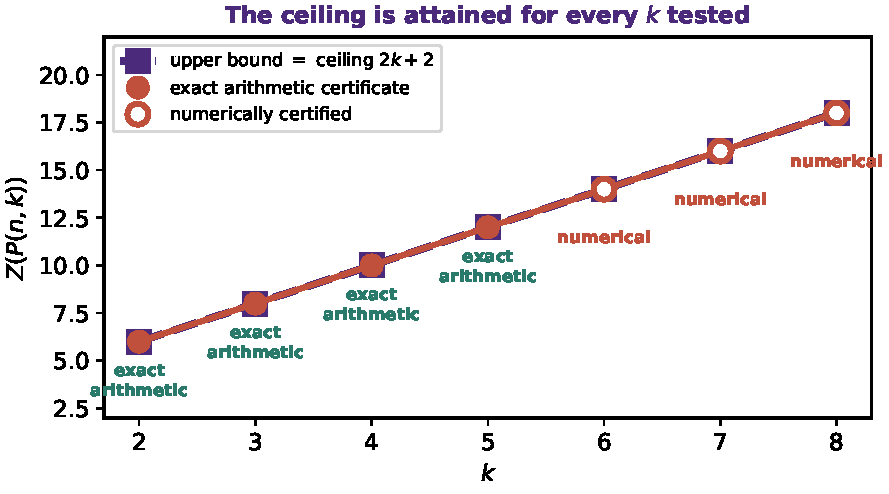
\includegraphics[width=0.92\textwidth]{figures/fig_status.pdf}
\caption{How claims are classified in this project: proved, computed exactly, certified by interval arithmetic, numerical, refuted, open.}
\label{fig:status}
\end{figure}

\begin{thmbox}{The arc, in one paragraph}
$P(n,k)$ is a cyclic cover of a two-vertex base, so everything about it decomposes into $2\times2$ blocks over the characters of $\mathbb Z_n$ (Section 3). Over \emph{one} matrix --- the adjacency matrix --- that decomposition turns the Riemann Hypothesis for the Ihara zeta function into the sign of one integer polynomial on a cosine grid, then into one fixed region $Q\ge0$ that does not depend on $k$, then via Dirichlet into a finite problem in both variables, which is exhausted exactly (Section 12). Over \emph{every} matrix with the pattern, eliminating the inner coordinates leaves a recurrence of order $2k+2$, so the certificate method either matches the rotation-bootstrap upper bound exactly or cannot (Section 6); period-one certificates match it on divisibility classes (Sections 7--8), identity tiles match it for every large $n$ (Section 9), and Krawczyk certification in exact rational arithmetic makes that a theorem (Section 9). On general cyclic covers the ceiling holds for equivariant matrices with nonvanishing symbol and for every matrix on three families of bases, fails on arbitrary bases and on regular bases, and the condition the proofs actually use --- a monomial leading coefficient of the symbol --- is proved to be sufficient on every base, with the strip kernel of dimension exactly the span (Section 10).
\end{thmbox}

\subsection{Status of every claim (matching the paper's Status section)}

\begin{itemize}[leftmargin=*]
  \item \textbf{Proved.} The rotation bootstrap (Thm 4.1); the inner elimination and monodromy formula (Thms 6.1, 6.2) and the ceiling $M\le M_{\mathrm{cs}}\le2k+2$ (Cor 6.3); the Fourier blocks and the three-parameter symbol (Thms 7.1, 7.2); realisability and the antipodal obstruction; the cyclotomic certificate theorem (Thm 8.1) and the adjacency nullity classification (Thm 8.2); period-one confinement to divisibility classes (Thm 9.1); tile independence and the tiling theorem (Lemma 9.2, Thm 9.3); the cover reduction \emph{with} its hypothesis (Thm 10.1) and attainment (Thm 10.2); the non-equivariant ceiling on two-vertex, path-with-loops and cycle bases (Thm 10.3); both refutations (Thms 10.4, 10.8); the independent-set and low-rank-subgraph obstructions (Props 10.5, 10.7); the period-one ceiling (Thm 11.2); in Part I, the criterion (Thm 12.3), corner criterion (Thm 12.5), finiteness three ways (Thms 12.6, 12.7), locality (Thm 12.9), the two cover criteria and the no-go (Thms 12.10, 12.11), and the deficit bound (Prop 12.12).
  \item \textbf{Proved by an exact certificate.} $Z(P(n,2))=6$ for $n\ge9$, $n\ne10$, and $n\in7\mathbb Z$; $Z(P(n,3))=8$ for $n\in10\mathbb Z$; $Z(P(n,4))=10$ for $n\in60\mathbb Z\cup70\mathbb Z\cup90\mathbb Z$; $Z(P(n,5))=12$ for $n\in24\mathbb Z$; $Z(P(n,7))=16$ for $n\in120\mathbb Z$; $M(P(10,2))=6$ (Thm 11.3); the nullity-$6$ integer matrix on the $K_4$ covers; the rank-one matrices of Thm 10.8 at $n=4,\dots,10$; and the complete Ramanujan classification, all $\RamAllCases$ cases (Thm 12.8).
  \item \textbf{Proved by interval certification, evaluated exactly.} $Z=M=8$ for every $n\ge17$ at $k=3$; $Z=M=10$ for every $n\ge\SettleFour$ at $k=4$; $Z=M=12$ for every $n\ge\SettleFive$ at $k=5$ (Thm 9.5): $\NtileAll$ tiles and $\NcertGN$ per-$n$ matrices, $\alpha\le\MaxAlpha$.
  \item \textbf{Proved (finite).} Every tabulated $Z$ by exhaustive search; with the above, $Z(P(n,k))$ is determined for every $n$ at $k=2,3,4$ (Thm 9.6), and $Z(P(n,3))=8$ for every $n\ge13$ with $13$ optimal --- Krishnan's Conjecture 5.
  \item \textbf{Numerical, not exact.} $Z(P(n,6))=14$ at $n=60,72,84,90,96,108,120$ and $Z(P(96,8))=18$; the nullity-$(n+1)$ witness on the $K_4$ cover at $n=4$.
  \item \textbf{Observation supported by computation.} The rank law $\operatorname{rank}J=\min(2d+1,k+1)$ for $3\le k\le13$, $d\le7$; the symplectic structure of tile products.
  \item \textbf{Conjectural.} The existence of a threshold $N(k)$ for every $k\ge6$; the cover ceiling when $c_{\max}$ has two or more monomials.
  \item \textbf{Refuted (ours).} That period-one certificates never exceed nullity $6$ (Section 8); the cover ceiling for arbitrary bases (Thm 10.4); the cover ceiling for \emph{regular} bases and the conjecture $M=6$ on the $K_4$ family, which had been presented as the project's strongest result (Thm 10.8); the statement that the equivariant maximum nullity there is $6$ (false because Thm 10.1 needs $\det M(\zeta)\not\equiv0$); a strict gap at $P(10,2)$ (Thm 11.3); the threshold form $n_0(k)=5k-2$ (by $Z(P(29,6))=12$); any bound $Z\le2(\gcd(n,j)+\gcd(n,k))$ (by $Z(P(11,3))=7$); an invalid Taylor-expansion proof of the uniform constant $\pi(2+\sqrt2)$ (the constant was right, the argument was not).
  \item \textbf{Withdrawn as unreliable.} An eigenvalue-minimising search whose plateaus were reported as evidence that the ceiling is unreachable at various $(n,k)$; it gave $7$ at $P(20,3)$ where $8$ is attained.
  \item \textbf{Open.} Tiles for $k\ge6$; whether $M(B^n)$ on the $K_4$ family is $n$, $n+1$ or $n+2$; $M(P(24,4))$ (period-one cannot reach it, Thm 11.2; tiling is unaffected); whether $M=Z$ on every $P(n,k)$; a closed form for the Ramanujan list.
\end{itemize}

\begin{callbox}{Three things to say about the whole project}
\begin{enumerate}[leftmargin=*,nosep]
  \item The two halves are one computation: a $2\times2$ block over each character of $\mathbb Z_n$. Fix the weights and ask about eigenvalues --- Part I. Free the weights and ask about the zero eigenvalue --- Part II.
  \item The certificate method on $P(n,k)$ has \emph{no slack}: its ceiling equals the known upper bound exactly, so it either settles $Z$ or cannot. It settles it at $k=2,3,4$.
  \item The project's own record contains more refutations than most papers: a false published theorem corrected by someone else and then proved for all $n$ here, and several conjectures of our own found false --- one by the verification suite, one by reasoning about pendant vertices, and one by an outside reader noticing a triangle.
\end{enumerate}
\end{callbox}

\vspace{0.6cm}
\begin{center}
\textbf{--- End of the Mathematical Reference Manual ---}
\end{center}

\begin{thebibliography}{99}
\bibitem{RST} S. Rashidi, N. Shajareh Poursalavati, M. Tavakkoli, Computing the zero forcing number for generalized Petersen graphs, \emph{J. Algebra Combin. Discrete Struct. Appl.} 7(2) (2020), 183--193.
\bibitem{K} A. Krishnan, A correction to the zero forcing number of the generalized Petersen graphs $P(n,3)$, arXiv:2607.19412 (2026).
\bibitem{AIM} AIM Minimum Rank -- Special Graphs Work Group, Zero forcing sets and the minimum rank of graphs, \emph{Linear Algebra Appl.} 428 (2008), 1628--1648.
\bibitem{FH} S. Fallat, L. Hogben, Variants on the minimum rank problem: a survey II, arXiv:1102.5142.
\bibitem{AVG} S. Akbari, E. Vatandoost, Y. Golkhandy Pour, Maximum nullity and zero forcing number on cubic graphs, arXiv:1705.09773.
\bibitem{BDHSY} D. Burgarth, D. D'Alessandro, L. Hogben, S. Severini, M. Young, Zero forcing, linear and quantum controllability for systems evolving on networks, \emph{IEEE Trans. Automat. Control} 58 (2013), 2349--2354.
\bibitem{CJ} J. H. Conway, A. J. Jones, Trigonometric Diophantine equations (On vanishing sums of roots of unity), \emph{Acta Arith.} 30 (1976), 229--240.
\bibitem{GS} R. Gera, P. St\u{a}nic\u{a}, The spectrum of generalized Petersen graphs, \emph{Australas. J. Combin.} 49 (2011), 39--45.
\bibitem{Terras} A. Terras, \emph{Zeta Functions of Graphs: A Stroll through the Garden}, Cambridge University Press, 2010.
\bibitem{LS} T. A. Le, J. W. Sander, Integral circulant Ramanujan graphs of prime power order, \emph{Electron. J. Combin.} 20 (2013), \#P35.
\bibitem{LPS} A. Lubotzky, R. Phillips, P. Sarnak, Ramanujan graphs, \emph{Combinatorica} 8 (1988), 261--277.
\bibitem{MKC} R. E. Moore, R. B. Kearfott, M. J. Cloud, \emph{Introduction to Interval Analysis}, SIAM, 2009.
\bibitem{GT} J. L. Gross, T. W. Tucker, \emph{Topological Graph Theory}, Dover, 2001.
\end{thebibliography}

\end{document}
